% Options for packages loaded elsewhere
\PassOptionsToPackage{unicode}{hyperref}
\PassOptionsToPackage{hyphens}{url}
%
\documentclass[
]{article}
\usepackage{lmodern}
\usepackage{amssymb,amsmath}
\usepackage{ifxetex,ifluatex}
\ifnum 0\ifxetex 1\fi\ifluatex 1\fi=0 % if pdftex
  \usepackage[T1]{fontenc}
  \usepackage[utf8]{inputenc}
  \usepackage{textcomp} % provide euro and other symbols
\else % if luatex or xetex
  \usepackage{unicode-math}
  \defaultfontfeatures{Scale=MatchLowercase}
  \defaultfontfeatures[\rmfamily]{Ligatures=TeX,Scale=1}
\fi
% Use upquote if available, for straight quotes in verbatim environments
\IfFileExists{upquote.sty}{\usepackage{upquote}}{}
\IfFileExists{microtype.sty}{% use microtype if available
  \usepackage[]{microtype}
  \UseMicrotypeSet[protrusion]{basicmath} % disable protrusion for tt fonts
}{}
\makeatletter
\@ifundefined{KOMAClassName}{% if non-KOMA class
  \IfFileExists{parskip.sty}{%
    \usepackage{parskip}
  }{% else
    \setlength{\parindent}{0pt}
    \setlength{\parskip}{6pt plus 2pt minus 1pt}}
}{% if KOMA class
  \KOMAoptions{parskip=half}}
\makeatother
\usepackage{xcolor}
\IfFileExists{xurl.sty}{\usepackage{xurl}}{} % add URL line breaks if available
\IfFileExists{bookmark.sty}{\usepackage{bookmark}}{\usepackage{hyperref}}
\hypersetup{
  hidelinks,
  pdfcreator={LaTeX via pandoc}}
\urlstyle{same} % disable monospaced font for URLs
\usepackage[margin=1in]{geometry}
\usepackage{longtable,booktabs}
% Correct order of tables after \paragraph or \subparagraph
\usepackage{etoolbox}
\makeatletter
\patchcmd\longtable{\par}{\if@noskipsec\mbox{}\fi\par}{}{}
\makeatother
% Allow footnotes in longtable head/foot
\IfFileExists{footnotehyper.sty}{\usepackage{footnotehyper}}{\usepackage{footnote}}
\makesavenoteenv{longtable}
\usepackage{graphicx}
\makeatletter
\def\maxwidth{\ifdim\Gin@nat@width>\linewidth\linewidth\else\Gin@nat@width\fi}
\def\maxheight{\ifdim\Gin@nat@height>\textheight\textheight\else\Gin@nat@height\fi}
\makeatother
% Scale images if necessary, so that they will not overflow the page
% margins by default, and it is still possible to overwrite the defaults
% using explicit options in \includegraphics[width, height, ...]{}
\setkeys{Gin}{width=\maxwidth,height=\maxheight,keepaspectratio}
% Set default figure placement to htbp
\makeatletter
\def\fps@figure{htbp}
\makeatother
\setlength{\emergencystretch}{3em} % prevent overfull lines
\providecommand{\tightlist}{%
  \setlength{\itemsep}{0pt}\setlength{\parskip}{0pt}}
\setcounter{secnumdepth}{5}
\usepackage{amsmath,amsfonts,amssymb,amsthm}
\usepackage{tikz}
\usetikzlibrary{positioning}

\usepackage{longtable}
\usepackage{booktabs}
\usepackage{caption}
\usepackage{subcaption}
\usepackage{rotating}
\usepackage{float}
\theoremstyle{plain}
\newtheorem{theorem}{Theorem}[section]
\newtheorem{corollary}[theorem]{Corollary}
\usepackage{booktabs}
\usepackage{longtable}
\usepackage{array}
\usepackage{multirow}
\usepackage{wrapfig}
\usepackage{float}
\usepackage{colortbl}
\usepackage{pdflscape}
\usepackage{tabu}
\usepackage{threeparttable}
\usepackage{threeparttablex}
\usepackage[normalem]{ulem}
\usepackage{makecell}
\ifluatex
  \usepackage{selnolig}  % disable illegal ligatures
\fi
\newlength{\cslhangindent}
\setlength{\cslhangindent}{1.5em}
\newlength{\csllabelwidth}
\setlength{\csllabelwidth}{3em}
\newenvironment{CSLReferences}[3] % #1 hanging-ident, #2 entry spacing
 {% don't indent paragraphs
  \setlength{\parindent}{0pt}
  % turn on hanging indent if param 1 is 1
  \ifodd #1 \everypar{\setlength{\hangindent}{\cslhangindent}}\ignorespaces\fi
  % set entry spacing
  \ifnum #2 > 0
  \setlength{\parskip}{#2\baselineskip}
  \fi
 }%
 {}
\usepackage{calc} % for \widthof, \maxof
\newcommand{\CSLBlock}[1]{#1\hfill\break}
\newcommand{\CSLLeftMargin}[1]{\parbox[t]{\maxof{\widthof{#1}}{\csllabelwidth}}{#1}}
\newcommand{\CSLRightInline}[1]{\parbox[t]{\linewidth}{#1}}
\newcommand{\CSLIndent}[1]{\hspace{\cslhangindent}#1}

\author{}
\date{\vspace{-2.5em}}

\begin{document}

{
\setcounter{tocdepth}{2}
\tableofcontents
}
\newpage

\hypertarget{introduction}{%
\section{Introduction}\label{introduction}}

\textcolor{red}{Title: Bounds in Two-Sample Mendelian Randomization With Summary Statistics: A Guide to Practice? or Promises and Pitalls?}

\textcolor{red}{I would use Bibtex to manage your references. This is almost always required for most journals.}

The gold standard to estimate the causal effect of a treatment or an exposure on an outcome is a randomized trial where the treatment assignment is randomized. However, in many epidemiological studies, randomized experiments are not feasible. For example, a study estimating the negative effects of smoking on depression (Wootton et al. 2019) would not be feasible with a randomized trial due to ethical concerns. In such settings, epidemiologists rely on different types of observational studies, which introduces potential biases from unmeasured confounders. In recent years, there has been an increase in using instrumental variable (IV) in the form of Mendelian randomization (MR) \textcolor{red}{Cite \url{https://academic.oup.com/ije/article/32/1/1/642797} and Lawlor et al. 2008} . Briefly, IV is a variable that is (A1) associated with the exposure, (A2) is independent from unmeasured confounders affecting the exposure and the outcome, and (A3) affects the outcome only through its effect on the exposure; see \ref{sec:iv-assumptions-and-two-sample-mr} for details. MR uses genetic variants, usually single nucleotide polymorphisms, as instruments to estimate the causal effect of an exposure on an outcome. This is based on the idea being that genotypes are randomly assigned when passed on from parents to offspring at meiosis (Lawlor et al. 2008) and thus, they make excellent candidates for satisfying (A2), especially when the exposure of interest is environmental.

MR analyses often use published summary statistics from two independent genome wide association studies \textcolor{red}{Cite Burgess, Butterworth, and Thompson's Mendelian randomization analysis...; Pierce and Burgess' efficient design for mendelian...; and Burgess et al's Using published data in mendelian randomization...;(Davies, Holmes, and Smith 2018)} \textcolor{red}{Not sure about these citations...we can discuss(Erlich and Narayanan 2014; Fuller et al. 1999; Wang et al. 2017)}. Typically, the first study provides information about the exposure and instrument and the second study provides information about the outcome and instrument. Once investigator have summary statistics from two studies,  they use methods based on parametric modeling assumptions \textcolor{red}{Cite \url{https://www.amazon.com/Mendelian-Randomization-Estimation-Interdisciplinary-Statistics/dp/1466573171} and \url{https://journals.sagepub.com/doi/full/10.1177/0962280215597579}} to arrive at point estimates and tests for the exposure effect.

An alternative approach to study the casual effect of the exposure without parametric assumptions is through non-parametric IV bounds (Robins (1989), Manski (1990), Balke and Pearl (1997), Richardson and Robins (2014), Cheng and Small (2006)) \textcolor{red}{cite cheng and small} Briefly, nonparametric IV bounds only use the bare minimum amount of assumptions, usually (A1)-(A3), to provide a range of plausible values for the exposure effect. They are typically used when the outcome, the exposure, and the instrument are all binary and are simultaneously observed. The most well-known are the Balke-Pearl bounds for the average treatment effect under slight variants of assumptions (A1)-(A3), and a set of instrumental inequalities to falsify the IV assumptions. Since then, Cheng and Small (2006) and Richardson and Robins (2014) extended the Balke-Pearl bounds to allow for a non-binary instrument. Ramsahai 2012 derived bounds for the two-sample setting where the exposure and instrument are observed from one study and the outcome and instrument are observed from another study. %\textcolor{red}{cite R package for this} provides software to compute IV bounds for two-sample MR studies using only summary statistics.
For a recent overview, see Swanson et al. (2018). 

Due to their nonparametric nature, the IV bounds are attractive approaches to analyze exposure effects especially if some modeling assumptions are suspect or difficult to justify. In MR, the minimal set of assumptions needed for non-parametric bounds is a stark contrast to many other MR approaches, such as the IVW estimator \textcolor{red}{Cite Burgess, S., Butterworth, A., and Thompson, S. G. (2013). Mendelian randomization analysis...}, MR-Egger regression \textcolor{red}{Cite Bowden paper in Int Journal of Epi}, weighted median \textcolor{red}{Cite Bowden's paper in genetic epi} and modes \textcolor{red}{Hartwig's paper in Int Journal of Epi}, MRRAPs \textcolor{red}{cite recent AoS paper by Zhao et al. on RAPs}, and others, that make parametric assumptions about the exposure effect. More generally, if IV bounds using fewer assumptions arrive at similar conclusions about the exposure effect as those based on parametric approaches, the case for the causal effect on the exposure becomes stronger.

Despite their attractive properties, there is a poor understanding about the behavior of IV bounds in two-sample MR studies using only summary statistics. For example, what kind of genetic instruments are needed to provide useful conclusions about the exposure effect, say the bound does not contain the null effect? Can combining multiple instruments lead to shorter and tighter bounds on the exposure effect? How does the shape of the bounds change if many instruments are very weak, which is typically the case in MR studies based on genetic instruments? In traditional setups for IV bounds where individual-level data consisting jointly of the outcome, the exposure, and a single instrument are available, the Balke-Pearl bounds are usually conservative and contain the null effect. However, it is not clear if the same principle holds for two-sample MR studies, especially if multiple candidate IVs are available. The goal of the paper is to address these questions and provide a more in-depth exploration of these bounds, specifically addressing what we can expect to learn and what information can be gained by utilizing multiple IVs under assumptions similar to Balke-Pearl bounds

The paper is divided as follows. Section \ref{} \textcolor{red}{Fill this after done}.

%(see for example (Beck, Shorter, and Brookes 2020)), which often include data on just one variable together with genetic markers. 


\hypertarget{setup}{%
\section{Setup}\label{setup}}

\hypertarget{notation-and-definitions}{%
\subsection{Review: Notation, Assumptions, and Definitions}\label{notation-and-definitions}}

In the following, let \(X\) and \(Y\) be binary exposure and outcome, respectively, \(Z\) be a categorical instrumental variable taking values in \{0, 1, and 2\}, and \(U\) an unmeasured confounder for the effect of \(X\) on \(Y\). No assumptions about the structure of \(U\) are made. Let \(Y^{z,x}\) be the potential outcome \textcolor{red}{Cite Neyman 1923 and Rubin's Estimating Causal Effects of Treatment in Randomized... (1974)} had the subject received exposure value \(X = x\) and instrument value \(Z = z\). Let \(X^z\) be the potential exposure had the subject received instrument value \(X\) if \(Z = z\). To link the potential outcomes to the observed data, we assume the stable unit treatment value assumption (SUTVA) \textcolor{red}{Cite Cox (1958), Rubin's original 1980 work on this} where $Y = \sum_{x,z} I[Z = z, X = x] Y^{x,z}$, $X = \sum_z I[Z=z] X^{z}$, and $I[\cdot]$ is the indicator function.

We make the following set of assumptions about the instrument, the exposure, and the outcome that are typical in MR studies.
\begin{itemize}
\tightlist
\item[(A1)] \emph{(Relevance)}: $Z \not\perp X$ 
\item[(A2)] \emph{(Ignorable instrument)}: $Z \perp U, Y^{z,x}$ for all $x,z$  % which implies \(Z \perp Y^{z,x}\) for all \(x,z\).
\item[(A3)] \emph{(Exclusion restriction)}: $Y^{z,x} = Y^{z',x} = Y^{x}$ for all $x,z,z'$ 
\end{itemize}
Briefly, assumption (A1) can be assessed finding SNPs that have been consistently associated with the exposure through multiple GWAS (Marigorta et al. 2018). Assumption (A2) is usually assumed to hold based on the premise that, conditional on parents' genotype, an offspring's genotype is often randomly assigned at conception. Assumption (A3) states that there is no direct effect of the instrument \(Z\) on the outcome \(Y\) other than that through the exposure \(X\) and like assumption (A2), is assumed to hold in some MR studies. Both assumptions (A2) and (A3) are potentially violated if the SNP is in linkage disequilibrium with an unmeasured SNP that affects the exposure and outcome, if the SNP is pleiotropic and has multiple functions beyond affecting the exposure, or through population stratification. For a more in-depth discussion of the validity of some of these assumptions in a Mendelian randomization setting, see Lawlor et al. (2008).

We also state two assumptions that will be referenced throughout this paper and help us explain the behavior of the IV bounds.
\begin{itemize}
\item[(A5)] \emph{(Monotonicity between $Z$ and $X$)} $P(X = 1 | Z = z, U) \le P(X = 1 | Z = z+1, U)$
\item[(A6)] \emph{(Monotonicity between $Z$ and $Y$)} $P(Y = 1 | Z = z, U) \le P(Y = 1 | Z = z+1, U)$
\end{itemize}
Assumption (A5) is common in the IV literature on using IVs to study noncompliance \textcolor{red}{Cite Angrist, Imbens, Rubin 1996 and Baiocchi, Cheng, and Small review paper in stat med}. Assumption (A6) is an extension of assumption (A5) to the outcome. Both are plausible in MR if the direction of the effects of the genetic instrument on the exposure and/or the outcome are well-established. 

Next, we introduce two designs of MR studies, the bivariate design \textcolor{red}{maybe we should call it two-sample design to be consistent with literature?} and the trivariate design \textcolor{red}{one-sample design?}. The bivariate design has two separate data sources, one providing information of \((X,Z)\) and one providing information of \((Y,Z)\), and is the most popular design in MR studies. The trivariate design has a single data source providing information on all observed variables \((X,Y,Z)\) and is more common in traditional studies of nonparametric IV bounds. \textcolor{red}{briefly discuss summary stat's role?}

Finally, we conclude the section by defining the target quantity of interest and instrument strength. First, we are interested in bounding the average treatment effect (ATE)
\[
\text{ATE} = E[Y^1 - Y^0].
\]
It is well-known that additional assumptions beyond (A1)-(A3) are needed to point-identify the ATE; see \textcolor{red}{Baiocchi, Cheng, and Small (cite) for details}. Even under assumption (A5), the ATE cannot be point-identified. Second, we define the strength of the IV $Z$ on the exposure $X$ as the maximum possible contrast between the exposure when instruments take on different values 
\[
\(\text{ST} = \max_{z_1,z_2} | P(X = 1 | Z = z_1) - P(X = 1 | Z = z_2) |\)
\]
ST matches the definition of strength in Balke and Pearl when the instrument is binary, but differs from other definitions of strength when a parametric model is assumed, say instrument strength based on the concentration parameter; \textcolor{red}{see Stock et al. (review paper on weak IV, in JBES, early 2000, highly cited)} for an overview.

\hypertarget{bounds-on-average-treatment-effect}{%
\subsection{Bounds on Average Treatment Effect}\label{bounds-on-average-treatment-effect}}

We will briefly review the method presented by Ramsahai (2012). Since our main focus is the bivariate data setting, we will demonstrate the method in this setting here. Similar arguments can be made to arrive at bounds from trivariate data.

Let \(\vec{\tau}^* = \Big(P(Y = 1 | X = 0, U), P(Y = 1 | X = 1, U), P(X = 1 | Z = 0, U), ..., P(X = 1 | Z = k-1, U)\Big) \in [0,1]^{2+k}\) and \(\vec{v}^* = \Big(P(Y = 0 | Z = 0, U), ..., P(Y = 1 | Z = k-1, U), P(X = 0 | Z = 0, U), ..., P(X = 1 | Z = k-1, U), \alpha^*\Big)\) where

\[
\begin{aligned}
\alpha^* &= P(Y = 1 | X = 1, U) - P(Y = 1 | X = 0, U).
\end{aligned}
\]

Since \(U \perp Z\), \(E_U[P(X = x | Z = z, U)] = P(X = x | Z = z)\) and \(E_U[P(Y = y | Z = z, U)] = P(Y = y | Z = z)\). Let \(\vec{v} = E_U[\vec{v}^*] = \Big(P(Y = 0 | Z = 0), ..., P(Y = 1 | Z = k-1), P(X = 0 | Z = 0), ..., P(X = 1 | Z = k-1), \alpha \Big)\), where

\[
\begin{aligned}
\alpha &= E_U[P(Y = 1 | X = 1, U) - P(Y = 1 | X = 0, U)] \\
       &= E[Y^1] - E[Y^0] = \text{ATE}.
\end{aligned}
\]

Note that while \(\vec{\tau}^*\) and \(\vec{v}^*\) are both entirely unobervable, \(\vec{v}\) consists of \(k\) observable values, and one unobservable value, the ATE.

By Marginal Excheangeability of \(Y^{z,x}\) \eqref{eq:marg-exch},

\[
P(X = x, Y = y | Z = z, U) = P(Y = 1 | X = x, U) P(X = x | Z = z, U),
\]

which means we can define a mapping \(f:[0,1]^{2+k} \mapsto \mathcal{V}\) such that \(f(\vec{\tau}^*) = \vec{v^*}\) as

\[
f(y_0, y_1, x_0, x_1, ..., x_{k-1}) = 
  \begin{pmatrix} 
    (1-y_0)\cdot(1-x_0) + (1 - y_1)\cdot x_0 \\
    y_0\cdot (1-x_0) + y_1\cdot x_0 \\
    \vdots \\
    (1-y_0)\cdot(1-x_{k-1}) + (1 - y_1)\cdot x_{k-1} \\
    y_0\cdot (1-x_{k-1}) + y_1\cdot x_{k-1} \\
  \end{pmatrix} \label{eq:f}
\]

We define \(\mathcal{V} = f([0,1]^{2+k})\).

Since \(\vec{v} = E_U[\vec{v}^*]\), \(\vec{v}\) must be a convex combination of \(\vec{v}^*\). Let \(\mathcal{H}\) be the convex hull of \(\mathcal{V}\). Then \(\vec{v}\) will be in \(\mathcal{H}\).

Now, let \(\hat{\mathcal{T}}\) be the set of extreme vertices of \([0,1]^{2+k}\), \(\hat{\mathcal{V}} = f(\hat{\mathcal{T}})\), and \(\hat{\mathcal{H}}\) be the convex hull of \(\hat{\mathcal{V}}\). By Theorem 1 in Appendix B of Ramsahai (2012), \(\mathcal{H} = \mathcal{\hat{H}}\). This means that \(\vec{v} \in \mathcal{\hat{H}}\). Utilizing a program such as Polymake, we can describe \(\mathcal{H}\) with a set of inequalities, which give us constraints that \(\vec{v}\) must satisfy.

This means that we can obtain inequalities that the components of \(\vec{v}\) must satisfy by describing the extreme vertices of \([0,1]^{2+k}\), map them to \(\mathcal{V}\) using the relatively simple function \(f\), and then use polymake to find inequalities that characterize the convex hull of \(f([0,1])^{2+k}\). This gives us a set of inequalities involving the components of \(\vec{v}\). Some of these will be verifiable, as they will not include the only unobservable quantity \(\alpha\). Others will not be verifiable, but will allow us to obtain bounds on the unobservable quantity \(\alpha\) using the observable entries of \(\vec{v}\).

This exact same approach can be used in the trivariate setting, and when imposing different extra assumptions, such as monotonicity of the effect of \(Z\) on \(X\) \eqref{eq:x_monotone} or \(Z\) on \(Y\) \eqref{eq:y_monotone}. The latter is done by imposing these assumption on \(\hat{\mathcal{V}}\) by removing vectors that violate these extra assumptions.

One important thing to note here is that these expressions do not always result in a valid set of bounds. In our simulations we found that a small fraction of the simulated probability distributions result in bounds where the lower limit is larger than the upper limit. Whether this is a problem in practice remains to be seen, but we are not aware of any real life data sets giving rise to bounds with this behavior. The cause for this is not clear, but among possible explanations is the existence of an assumption that is not captured in the checkable constraints. It is only natural to conclude that one or more assumptions are violated when one encounters a scenario where the bounds are flipped. For more, see Appendix \ref{exploration-of-scenarios-where-bounds-are-flipped}.

We implemented this approach using \texttt{R} version 4.0.2 (R Core Team 2020) for the high level calculations, and Polymake (Assarf et al. 2017) to obtain the inequalities.

\hypertarget{properties-of-bounds-from-summary-level-data}{%
\section{Properties of Bounds from Summary-Level Data}\label{properties-of-bounds-from-summary-level-data}}

Non-parametric bounds obtained from trivariate data sources have been thoroughly explored in the past for binary instruments. These bounds come with a few very desirable properties. For one, under the assumptions presented in Section \ref{iv-assumptions-and-two-sample-mr}, the width is guaranteed to be less than \(1 - \text{ST} = P(X = 0 | Z = 1) - P(X = 1 | Z = 0)\) (Balke and Pearl 1993). The bounds are computationally easy to calculate, and rely only on summary level data. In particular, with values of \(P(X = x, Y = y | Z = z)\), non-parametric bounds can be obtained. As mentioned, this allows us to avoid many of the privacy concerns that often arise when handling genetic data.

Scenarios where \(k > 2\) has, to our knowledge, not been thoroughly explored. Richardson and Robins (2014) provide bounds for a general categorical instrumental variable, but the behavior of these is not described in detail. Since the main scope of this paper is to explore bounds from bivariate data sources, we will not spend much time on the trivariate case, but will note that, from simulations, it seems like the width of trivariate bounds are indeed still bounded by \(1 - \text{ST}\) for \(k=3\) and \(k=4\) (Figure \ref{fig:trivariate-bound-on-width}).

\begin{figure}[H]
  \center
  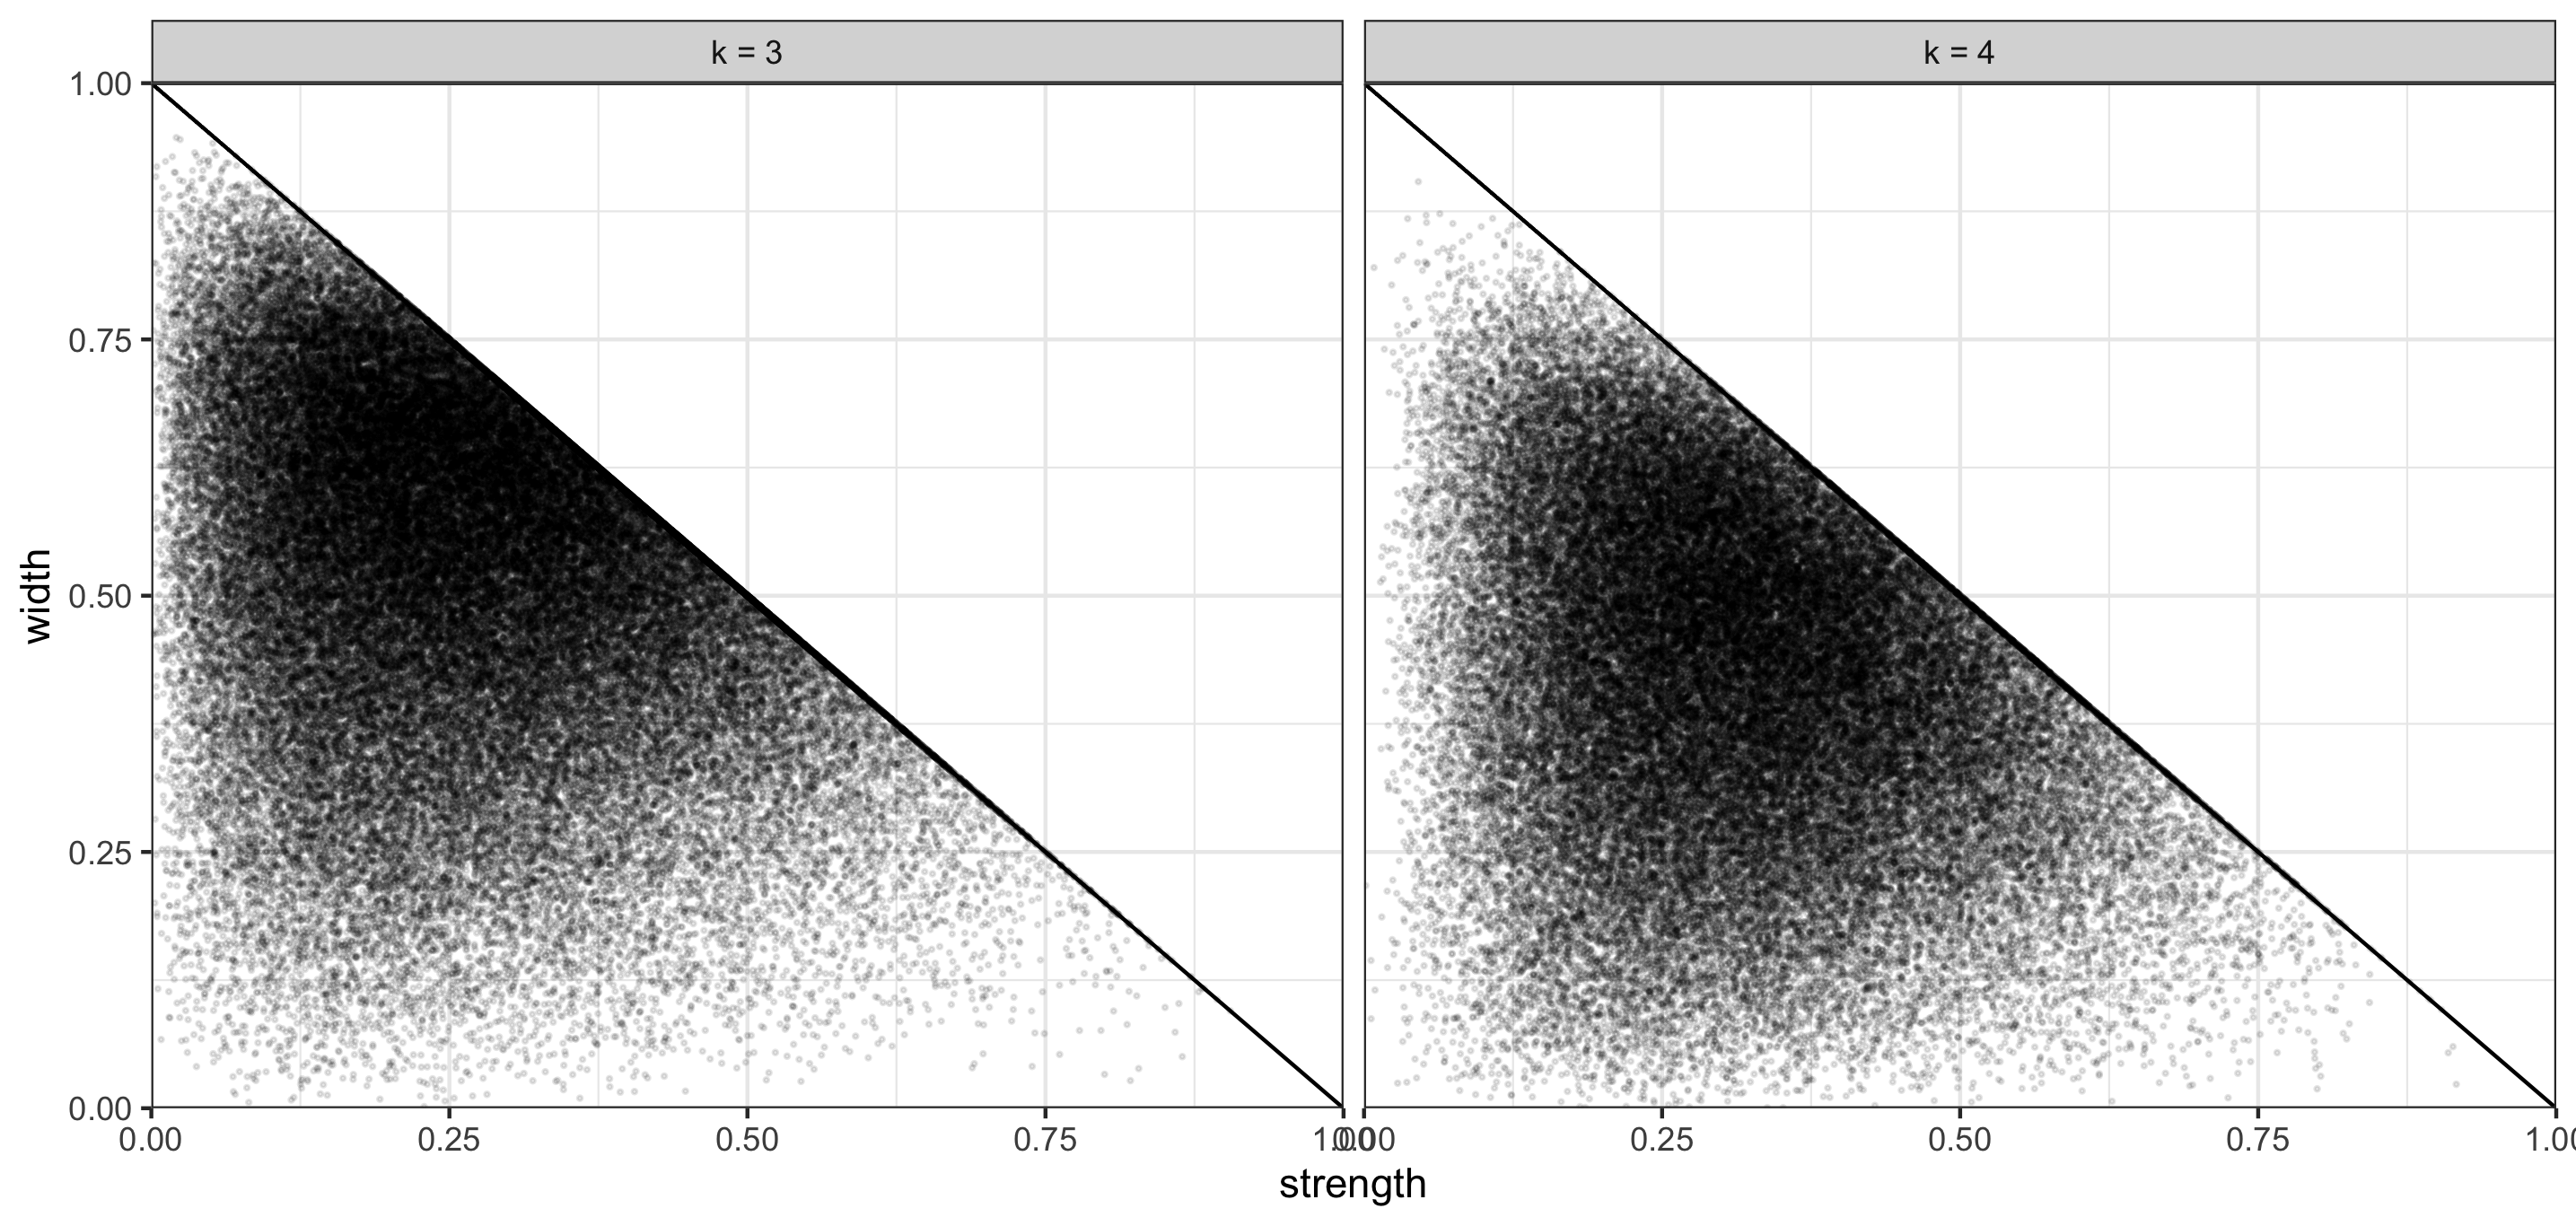
\includegraphics[width = 0.99\linewidth]{/Users/ralphtrane/Documents/RPackages_dev/ACEBounds/figures/trivariate_widths_vs_strengths.png}
  \caption{The results of calculating widths of bounds. \ensuremath{10^{5}} distributions of $(X,Y|Z)$ were randomly generated for both $k = 3$ and $k = 4$. For $k = 3$, 11,741 of these violated one or more of the constraints. For $k = 4$, 21,779 violated one or more of the constraints, and 37 resulted in an upper bound that is smaller than the lower bound. These are not included here. Black line indicates $\text{Width} = 1-\text{ST}$.}
  \label{fig:trivariate-bound-on-width}
\end{figure}

In Mendelian randomization, trivariate data sources are scarce. Bivariate data sources, on the other hand, are plentiful. The rest of this section is dedicated to explore the behavior of non-parametric bounds derived from bivariate data sources. These were first introduced by Ramsahai (2007).

\hypertarget{bounds-from-bivariate-data}{%
\subsection{Bounds from Bivariate Data}\label{bounds-from-bivariate-data}}

First, we seek to examine the information one can potentially obtain from bounds found using a single instrumental variable, when only summaries from bivariate data are available. We are particularly interested in whether we can gain any insights into the direction and magnitude of the ATE. One crucial quantity in this quest is the width of the bounds obtained. Wide bounds provide less information about the magnitude, and are much less likely to provide any information regarding direction as compared to narrower bounds. Here, we will first illustrate the application of the technique described in Section \ref{bounds-on-average-treatment-effect} before considering the behavior of these by constructing bounds from many sets of randomly generated values of \(P(X = 1 | Z = z)\) and \(P(Y = 1 | Z = z)\).

Following the approach from Ramsahai (2012) as outlined in Section \ref{bounds-on-average-treatment-effect}, we obtain bounds on the average treatment effect from the quantities \(P(X = 1 | Z = z)\) and \(P(Y = 1 | Z = z)\), \(z = 0,1,2\). To do so, we first write down the most extreme values of each of \(P(Y = 1 | X = x, U)\) and \(P(X = x | Z = z, U)\) for all \(x=0,1\), \(z=0,1,2\). Since these are probabilities, the extreme values are \(0\) and \(1\).

\begin{longtable}[]{@{}ccccc@{}}
\caption{Most extreme values of \(P(Y = 1 | X = x, U)\) and \(P(X = 1 | Z = z, U)\). Here, PY1XxU = \(P(Y = 1 | X = x, U)\) and PX1ZzU = \(P(X = 1 | Z = z, U)\).}\tabularnewline
\toprule
\begin{minipage}[b]{0.11\columnwidth}\centering
PY1X0U\strut
\end{minipage} & \begin{minipage}[b]{0.11\columnwidth}\centering
PY1X1U\strut
\end{minipage} & \begin{minipage}[b]{0.11\columnwidth}\centering
PY1Z0U\strut
\end{minipage} & \begin{minipage}[b]{0.11\columnwidth}\centering
PX1Z1U\strut
\end{minipage} & \begin{minipage}[b]{0.11\columnwidth}\centering
PX1Z2U\strut
\end{minipage}\tabularnewline
\midrule
\endfirsthead
\toprule
\begin{minipage}[b]{0.11\columnwidth}\centering
PY1X0U\strut
\end{minipage} & \begin{minipage}[b]{0.11\columnwidth}\centering
PY1X1U\strut
\end{minipage} & \begin{minipage}[b]{0.11\columnwidth}\centering
PY1Z0U\strut
\end{minipage} & \begin{minipage}[b]{0.11\columnwidth}\centering
PX1Z1U\strut
\end{minipage} & \begin{minipage}[b]{0.11\columnwidth}\centering
PX1Z2U\strut
\end{minipage}\tabularnewline
\midrule
\endhead
\begin{minipage}[t]{0.11\columnwidth}\centering
0\strut
\end{minipage} & \begin{minipage}[t]{0.11\columnwidth}\centering
0\strut
\end{minipage} & \begin{minipage}[t]{0.11\columnwidth}\centering
0\strut
\end{minipage} & \begin{minipage}[t]{0.11\columnwidth}\centering
0\strut
\end{minipage} & \begin{minipage}[t]{0.11\columnwidth}\centering
0\strut
\end{minipage}\tabularnewline
\begin{minipage}[t]{0.11\columnwidth}\centering
0\strut
\end{minipage} & \begin{minipage}[t]{0.11\columnwidth}\centering
0\strut
\end{minipage} & \begin{minipage}[t]{0.11\columnwidth}\centering
0\strut
\end{minipage} & \begin{minipage}[t]{0.11\columnwidth}\centering
0\strut
\end{minipage} & \begin{minipage}[t]{0.11\columnwidth}\centering
1\strut
\end{minipage}\tabularnewline
\begin{minipage}[t]{0.11\columnwidth}\centering
0\strut
\end{minipage} & \begin{minipage}[t]{0.11\columnwidth}\centering
0\strut
\end{minipage} & \begin{minipage}[t]{0.11\columnwidth}\centering
0\strut
\end{minipage} & \begin{minipage}[t]{0.11\columnwidth}\centering
1\strut
\end{minipage} & \begin{minipage}[t]{0.11\columnwidth}\centering
0\strut
\end{minipage}\tabularnewline
\begin{minipage}[t]{0.11\columnwidth}\centering
0\strut
\end{minipage} & \begin{minipage}[t]{0.11\columnwidth}\centering
0\strut
\end{minipage} & \begin{minipage}[t]{0.11\columnwidth}\centering
0\strut
\end{minipage} & \begin{minipage}[t]{0.11\columnwidth}\centering
1\strut
\end{minipage} & \begin{minipage}[t]{0.11\columnwidth}\centering
1\strut
\end{minipage}\tabularnewline
\begin{minipage}[t]{0.11\columnwidth}\centering
0\strut
\end{minipage} & \begin{minipage}[t]{0.11\columnwidth}\centering
0\strut
\end{minipage} & \begin{minipage}[t]{0.11\columnwidth}\centering
1\strut
\end{minipage} & \begin{minipage}[t]{0.11\columnwidth}\centering
0\strut
\end{minipage} & \begin{minipage}[t]{0.11\columnwidth}\centering
0\strut
\end{minipage}\tabularnewline
\begin{minipage}[t]{0.11\columnwidth}\centering
0\strut
\end{minipage} & \begin{minipage}[t]{0.11\columnwidth}\centering
0\strut
\end{minipage} & \begin{minipage}[t]{0.11\columnwidth}\centering
1\strut
\end{minipage} & \begin{minipage}[t]{0.11\columnwidth}\centering
0\strut
\end{minipage} & \begin{minipage}[t]{0.11\columnwidth}\centering
1\strut
\end{minipage}\tabularnewline
\begin{minipage}[t]{0.11\columnwidth}\centering
0\strut
\end{minipage} & \begin{minipage}[t]{0.11\columnwidth}\centering
0\strut
\end{minipage} & \begin{minipage}[t]{0.11\columnwidth}\centering
1\strut
\end{minipage} & \begin{minipage}[t]{0.11\columnwidth}\centering
1\strut
\end{minipage} & \begin{minipage}[t]{0.11\columnwidth}\centering
0\strut
\end{minipage}\tabularnewline
\begin{minipage}[t]{0.11\columnwidth}\centering
0\strut
\end{minipage} & \begin{minipage}[t]{0.11\columnwidth}\centering
0\strut
\end{minipage} & \begin{minipage}[t]{0.11\columnwidth}\centering
1\strut
\end{minipage} & \begin{minipage}[t]{0.11\columnwidth}\centering
1\strut
\end{minipage} & \begin{minipage}[t]{0.11\columnwidth}\centering
1\strut
\end{minipage}\tabularnewline
\begin{minipage}[t]{0.11\columnwidth}\centering
0\strut
\end{minipage} & \begin{minipage}[t]{0.11\columnwidth}\centering
1\strut
\end{minipage} & \begin{minipage}[t]{0.11\columnwidth}\centering
0\strut
\end{minipage} & \begin{minipage}[t]{0.11\columnwidth}\centering
0\strut
\end{minipage} & \begin{minipage}[t]{0.11\columnwidth}\centering
0\strut
\end{minipage}\tabularnewline
\begin{minipage}[t]{0.11\columnwidth}\centering
0\strut
\end{minipage} & \begin{minipage}[t]{0.11\columnwidth}\centering
1\strut
\end{minipage} & \begin{minipage}[t]{0.11\columnwidth}\centering
0\strut
\end{minipage} & \begin{minipage}[t]{0.11\columnwidth}\centering
0\strut
\end{minipage} & \begin{minipage}[t]{0.11\columnwidth}\centering
1\strut
\end{minipage}\tabularnewline
\begin{minipage}[t]{0.11\columnwidth}\centering
0\strut
\end{minipage} & \begin{minipage}[t]{0.11\columnwidth}\centering
1\strut
\end{minipage} & \begin{minipage}[t]{0.11\columnwidth}\centering
0\strut
\end{minipage} & \begin{minipage}[t]{0.11\columnwidth}\centering
1\strut
\end{minipage} & \begin{minipage}[t]{0.11\columnwidth}\centering
0\strut
\end{minipage}\tabularnewline
\begin{minipage}[t]{0.11\columnwidth}\centering
0\strut
\end{minipage} & \begin{minipage}[t]{0.11\columnwidth}\centering
1\strut
\end{minipage} & \begin{minipage}[t]{0.11\columnwidth}\centering
0\strut
\end{minipage} & \begin{minipage}[t]{0.11\columnwidth}\centering
1\strut
\end{minipage} & \begin{minipage}[t]{0.11\columnwidth}\centering
1\strut
\end{minipage}\tabularnewline
\begin{minipage}[t]{0.11\columnwidth}\centering
0\strut
\end{minipage} & \begin{minipage}[t]{0.11\columnwidth}\centering
1\strut
\end{minipage} & \begin{minipage}[t]{0.11\columnwidth}\centering
1\strut
\end{minipage} & \begin{minipage}[t]{0.11\columnwidth}\centering
0\strut
\end{minipage} & \begin{minipage}[t]{0.11\columnwidth}\centering
0\strut
\end{minipage}\tabularnewline
\begin{minipage}[t]{0.11\columnwidth}\centering
0\strut
\end{minipage} & \begin{minipage}[t]{0.11\columnwidth}\centering
1\strut
\end{minipage} & \begin{minipage}[t]{0.11\columnwidth}\centering
1\strut
\end{minipage} & \begin{minipage}[t]{0.11\columnwidth}\centering
0\strut
\end{minipage} & \begin{minipage}[t]{0.11\columnwidth}\centering
1\strut
\end{minipage}\tabularnewline
\begin{minipage}[t]{0.11\columnwidth}\centering
0\strut
\end{minipage} & \begin{minipage}[t]{0.11\columnwidth}\centering
1\strut
\end{minipage} & \begin{minipage}[t]{0.11\columnwidth}\centering
1\strut
\end{minipage} & \begin{minipage}[t]{0.11\columnwidth}\centering
1\strut
\end{minipage} & \begin{minipage}[t]{0.11\columnwidth}\centering
0\strut
\end{minipage}\tabularnewline
\begin{minipage}[t]{0.11\columnwidth}\centering
0\strut
\end{minipage} & \begin{minipage}[t]{0.11\columnwidth}\centering
1\strut
\end{minipage} & \begin{minipage}[t]{0.11\columnwidth}\centering
1\strut
\end{minipage} & \begin{minipage}[t]{0.11\columnwidth}\centering
1\strut
\end{minipage} & \begin{minipage}[t]{0.11\columnwidth}\centering
1\strut
\end{minipage}\tabularnewline
\begin{minipage}[t]{0.11\columnwidth}\centering
1\strut
\end{minipage} & \begin{minipage}[t]{0.11\columnwidth}\centering
0\strut
\end{minipage} & \begin{minipage}[t]{0.11\columnwidth}\centering
0\strut
\end{minipage} & \begin{minipage}[t]{0.11\columnwidth}\centering
0\strut
\end{minipage} & \begin{minipage}[t]{0.11\columnwidth}\centering
0\strut
\end{minipage}\tabularnewline
\begin{minipage}[t]{0.11\columnwidth}\centering
1\strut
\end{minipage} & \begin{minipage}[t]{0.11\columnwidth}\centering
0\strut
\end{minipage} & \begin{minipage}[t]{0.11\columnwidth}\centering
0\strut
\end{minipage} & \begin{minipage}[t]{0.11\columnwidth}\centering
0\strut
\end{minipage} & \begin{minipage}[t]{0.11\columnwidth}\centering
1\strut
\end{minipage}\tabularnewline
\begin{minipage}[t]{0.11\columnwidth}\centering
1\strut
\end{minipage} & \begin{minipage}[t]{0.11\columnwidth}\centering
0\strut
\end{minipage} & \begin{minipage}[t]{0.11\columnwidth}\centering
0\strut
\end{minipage} & \begin{minipage}[t]{0.11\columnwidth}\centering
1\strut
\end{minipage} & \begin{minipage}[t]{0.11\columnwidth}\centering
0\strut
\end{minipage}\tabularnewline
\begin{minipage}[t]{0.11\columnwidth}\centering
1\strut
\end{minipage} & \begin{minipage}[t]{0.11\columnwidth}\centering
0\strut
\end{minipage} & \begin{minipage}[t]{0.11\columnwidth}\centering
0\strut
\end{minipage} & \begin{minipage}[t]{0.11\columnwidth}\centering
1\strut
\end{minipage} & \begin{minipage}[t]{0.11\columnwidth}\centering
1\strut
\end{minipage}\tabularnewline
\begin{minipage}[t]{0.11\columnwidth}\centering
1\strut
\end{minipage} & \begin{minipage}[t]{0.11\columnwidth}\centering
0\strut
\end{minipage} & \begin{minipage}[t]{0.11\columnwidth}\centering
1\strut
\end{minipage} & \begin{minipage}[t]{0.11\columnwidth}\centering
0\strut
\end{minipage} & \begin{minipage}[t]{0.11\columnwidth}\centering
0\strut
\end{minipage}\tabularnewline
\begin{minipage}[t]{0.11\columnwidth}\centering
1\strut
\end{minipage} & \begin{minipage}[t]{0.11\columnwidth}\centering
0\strut
\end{minipage} & \begin{minipage}[t]{0.11\columnwidth}\centering
1\strut
\end{minipage} & \begin{minipage}[t]{0.11\columnwidth}\centering
0\strut
\end{minipage} & \begin{minipage}[t]{0.11\columnwidth}\centering
1\strut
\end{minipage}\tabularnewline
\begin{minipage}[t]{0.11\columnwidth}\centering
1\strut
\end{minipage} & \begin{minipage}[t]{0.11\columnwidth}\centering
0\strut
\end{minipage} & \begin{minipage}[t]{0.11\columnwidth}\centering
1\strut
\end{minipage} & \begin{minipage}[t]{0.11\columnwidth}\centering
1\strut
\end{minipage} & \begin{minipage}[t]{0.11\columnwidth}\centering
0\strut
\end{minipage}\tabularnewline
\begin{minipage}[t]{0.11\columnwidth}\centering
1\strut
\end{minipage} & \begin{minipage}[t]{0.11\columnwidth}\centering
0\strut
\end{minipage} & \begin{minipage}[t]{0.11\columnwidth}\centering
1\strut
\end{minipage} & \begin{minipage}[t]{0.11\columnwidth}\centering
1\strut
\end{minipage} & \begin{minipage}[t]{0.11\columnwidth}\centering
1\strut
\end{minipage}\tabularnewline
\begin{minipage}[t]{0.11\columnwidth}\centering
1\strut
\end{minipage} & \begin{minipage}[t]{0.11\columnwidth}\centering
1\strut
\end{minipage} & \begin{minipage}[t]{0.11\columnwidth}\centering
0\strut
\end{minipage} & \begin{minipage}[t]{0.11\columnwidth}\centering
0\strut
\end{minipage} & \begin{minipage}[t]{0.11\columnwidth}\centering
0\strut
\end{minipage}\tabularnewline
\begin{minipage}[t]{0.11\columnwidth}\centering
1\strut
\end{minipage} & \begin{minipage}[t]{0.11\columnwidth}\centering
1\strut
\end{minipage} & \begin{minipage}[t]{0.11\columnwidth}\centering
0\strut
\end{minipage} & \begin{minipage}[t]{0.11\columnwidth}\centering
0\strut
\end{minipage} & \begin{minipage}[t]{0.11\columnwidth}\centering
1\strut
\end{minipage}\tabularnewline
\begin{minipage}[t]{0.11\columnwidth}\centering
1\strut
\end{minipage} & \begin{minipage}[t]{0.11\columnwidth}\centering
1\strut
\end{minipage} & \begin{minipage}[t]{0.11\columnwidth}\centering
0\strut
\end{minipage} & \begin{minipage}[t]{0.11\columnwidth}\centering
1\strut
\end{minipage} & \begin{minipage}[t]{0.11\columnwidth}\centering
0\strut
\end{minipage}\tabularnewline
\begin{minipage}[t]{0.11\columnwidth}\centering
1\strut
\end{minipage} & \begin{minipage}[t]{0.11\columnwidth}\centering
1\strut
\end{minipage} & \begin{minipage}[t]{0.11\columnwidth}\centering
0\strut
\end{minipage} & \begin{minipage}[t]{0.11\columnwidth}\centering
1\strut
\end{minipage} & \begin{minipage}[t]{0.11\columnwidth}\centering
1\strut
\end{minipage}\tabularnewline
\begin{minipage}[t]{0.11\columnwidth}\centering
1\strut
\end{minipage} & \begin{minipage}[t]{0.11\columnwidth}\centering
1\strut
\end{minipage} & \begin{minipage}[t]{0.11\columnwidth}\centering
1\strut
\end{minipage} & \begin{minipage}[t]{0.11\columnwidth}\centering
0\strut
\end{minipage} & \begin{minipage}[t]{0.11\columnwidth}\centering
0\strut
\end{minipage}\tabularnewline
\begin{minipage}[t]{0.11\columnwidth}\centering
1\strut
\end{minipage} & \begin{minipage}[t]{0.11\columnwidth}\centering
1\strut
\end{minipage} & \begin{minipage}[t]{0.11\columnwidth}\centering
1\strut
\end{minipage} & \begin{minipage}[t]{0.11\columnwidth}\centering
0\strut
\end{minipage} & \begin{minipage}[t]{0.11\columnwidth}\centering
1\strut
\end{minipage}\tabularnewline
\begin{minipage}[t]{0.11\columnwidth}\centering
1\strut
\end{minipage} & \begin{minipage}[t]{0.11\columnwidth}\centering
1\strut
\end{minipage} & \begin{minipage}[t]{0.11\columnwidth}\centering
1\strut
\end{minipage} & \begin{minipage}[t]{0.11\columnwidth}\centering
1\strut
\end{minipage} & \begin{minipage}[t]{0.11\columnwidth}\centering
0\strut
\end{minipage}\tabularnewline
\begin{minipage}[t]{0.11\columnwidth}\centering
1\strut
\end{minipage} & \begin{minipage}[t]{0.11\columnwidth}\centering
1\strut
\end{minipage} & \begin{minipage}[t]{0.11\columnwidth}\centering
1\strut
\end{minipage} & \begin{minipage}[t]{0.11\columnwidth}\centering
1\strut
\end{minipage} & \begin{minipage}[t]{0.11\columnwidth}\centering
1\strut
\end{minipage}\tabularnewline
\bottomrule
\end{longtable}

By applying the function \(f\), as presented in \eqref{eq:f}, to each row, we get the most extreme vertices of \(P(X = x | Z = z, U)\) and \(P(Y = y | Z = z, U)\) for all \(x=0,1,\ y=0,1\) and \(z=0,1,2\).

\begin{longtable}[]{@{}ccccccccccccc@{}}
\caption{Most extreme values of \(P(Y = y | Z = z)\) and \(P(X = x | Z = z, U)\). Here, PYyZzU = \(P(Y = y | Z = z, U)\), PXxZzU = \(P(X = x | Z = z, U)\), and \(\alpha = P(Y = 1 | X = 1,U) - P(Y = 1 | X = 0,U)\).}\tabularnewline
\toprule
\begin{minipage}[b]{0.05\columnwidth}\centering
PY0Z0\strut
\end{minipage} & \begin{minipage}[b]{0.05\columnwidth}\centering
PY0Z1\strut
\end{minipage} & \begin{minipage}[b]{0.05\columnwidth}\centering
PY0Z2\strut
\end{minipage} & \begin{minipage}[b]{0.05\columnwidth}\centering
PY1Z0\strut
\end{minipage} & \begin{minipage}[b]{0.05\columnwidth}\centering
PY1Z1\strut
\end{minipage} & \begin{minipage}[b]{0.05\columnwidth}\centering
PY1Z2\strut
\end{minipage} & \begin{minipage}[b]{0.05\columnwidth}\centering
PX0Z0\strut
\end{minipage} & \begin{minipage}[b]{0.05\columnwidth}\centering
PX0Z1\strut
\end{minipage} & \begin{minipage}[b]{0.05\columnwidth}\centering
PX0Z2\strut
\end{minipage} & \begin{minipage}[b]{0.05\columnwidth}\centering
PX1Z0\strut
\end{minipage} & \begin{minipage}[b]{0.05\columnwidth}\centering
PX1Z1\strut
\end{minipage} & \begin{minipage}[b]{0.05\columnwidth}\centering
PX1Z2\strut
\end{minipage} & \begin{minipage}[b]{0.07\columnwidth}\centering
\(\alpha\)\strut
\end{minipage}\tabularnewline
\midrule
\endfirsthead
\toprule
\begin{minipage}[b]{0.05\columnwidth}\centering
PY0Z0\strut
\end{minipage} & \begin{minipage}[b]{0.05\columnwidth}\centering
PY0Z1\strut
\end{minipage} & \begin{minipage}[b]{0.05\columnwidth}\centering
PY0Z2\strut
\end{minipage} & \begin{minipage}[b]{0.05\columnwidth}\centering
PY1Z0\strut
\end{minipage} & \begin{minipage}[b]{0.05\columnwidth}\centering
PY1Z1\strut
\end{minipage} & \begin{minipage}[b]{0.05\columnwidth}\centering
PY1Z2\strut
\end{minipage} & \begin{minipage}[b]{0.05\columnwidth}\centering
PX0Z0\strut
\end{minipage} & \begin{minipage}[b]{0.05\columnwidth}\centering
PX0Z1\strut
\end{minipage} & \begin{minipage}[b]{0.05\columnwidth}\centering
PX0Z2\strut
\end{minipage} & \begin{minipage}[b]{0.05\columnwidth}\centering
PX1Z0\strut
\end{minipage} & \begin{minipage}[b]{0.05\columnwidth}\centering
PX1Z1\strut
\end{minipage} & \begin{minipage}[b]{0.05\columnwidth}\centering
PX1Z2\strut
\end{minipage} & \begin{minipage}[b]{0.07\columnwidth}\centering
\(\alpha\)\strut
\end{minipage}\tabularnewline
\midrule
\endhead
\begin{minipage}[t]{0.05\columnwidth}\centering
1\strut
\end{minipage} & \begin{minipage}[t]{0.05\columnwidth}\centering
1\strut
\end{minipage} & \begin{minipage}[t]{0.05\columnwidth}\centering
1\strut
\end{minipage} & \begin{minipage}[t]{0.05\columnwidth}\centering
0\strut
\end{minipage} & \begin{minipage}[t]{0.05\columnwidth}\centering
0\strut
\end{minipage} & \begin{minipage}[t]{0.05\columnwidth}\centering
0\strut
\end{minipage} & \begin{minipage}[t]{0.05\columnwidth}\centering
1\strut
\end{minipage} & \begin{minipage}[t]{0.05\columnwidth}\centering
1\strut
\end{minipage} & \begin{minipage}[t]{0.05\columnwidth}\centering
1\strut
\end{minipage} & \begin{minipage}[t]{0.05\columnwidth}\centering
0\strut
\end{minipage} & \begin{minipage}[t]{0.05\columnwidth}\centering
0\strut
\end{minipage} & \begin{minipage}[t]{0.05\columnwidth}\centering
0\strut
\end{minipage} & \begin{minipage}[t]{0.07\columnwidth}\centering
0\strut
\end{minipage}\tabularnewline
\begin{minipage}[t]{0.05\columnwidth}\centering
0\strut
\end{minipage} & \begin{minipage}[t]{0.05\columnwidth}\centering
0\strut
\end{minipage} & \begin{minipage}[t]{0.05\columnwidth}\centering
0\strut
\end{minipage} & \begin{minipage}[t]{0.05\columnwidth}\centering
1\strut
\end{minipage} & \begin{minipage}[t]{0.05\columnwidth}\centering
1\strut
\end{minipage} & \begin{minipage}[t]{0.05\columnwidth}\centering
1\strut
\end{minipage} & \begin{minipage}[t]{0.05\columnwidth}\centering
1\strut
\end{minipage} & \begin{minipage}[t]{0.05\columnwidth}\centering
1\strut
\end{minipage} & \begin{minipage}[t]{0.05\columnwidth}\centering
1\strut
\end{minipage} & \begin{minipage}[t]{0.05\columnwidth}\centering
0\strut
\end{minipage} & \begin{minipage}[t]{0.05\columnwidth}\centering
0\strut
\end{minipage} & \begin{minipage}[t]{0.05\columnwidth}\centering
0\strut
\end{minipage} & \begin{minipage}[t]{0.07\columnwidth}\centering
-1\strut
\end{minipage}\tabularnewline
\begin{minipage}[t]{0.05\columnwidth}\centering
1\strut
\end{minipage} & \begin{minipage}[t]{0.05\columnwidth}\centering
1\strut
\end{minipage} & \begin{minipage}[t]{0.05\columnwidth}\centering
1\strut
\end{minipage} & \begin{minipage}[t]{0.05\columnwidth}\centering
0\strut
\end{minipage} & \begin{minipage}[t]{0.05\columnwidth}\centering
0\strut
\end{minipage} & \begin{minipage}[t]{0.05\columnwidth}\centering
0\strut
\end{minipage} & \begin{minipage}[t]{0.05\columnwidth}\centering
1\strut
\end{minipage} & \begin{minipage}[t]{0.05\columnwidth}\centering
1\strut
\end{minipage} & \begin{minipage}[t]{0.05\columnwidth}\centering
1\strut
\end{minipage} & \begin{minipage}[t]{0.05\columnwidth}\centering
0\strut
\end{minipage} & \begin{minipage}[t]{0.05\columnwidth}\centering
0\strut
\end{minipage} & \begin{minipage}[t]{0.05\columnwidth}\centering
0\strut
\end{minipage} & \begin{minipage}[t]{0.07\columnwidth}\centering
1\strut
\end{minipage}\tabularnewline
\begin{minipage}[t]{0.05\columnwidth}\centering
0\strut
\end{minipage} & \begin{minipage}[t]{0.05\columnwidth}\centering
0\strut
\end{minipage} & \begin{minipage}[t]{0.05\columnwidth}\centering
0\strut
\end{minipage} & \begin{minipage}[t]{0.05\columnwidth}\centering
1\strut
\end{minipage} & \begin{minipage}[t]{0.05\columnwidth}\centering
1\strut
\end{minipage} & \begin{minipage}[t]{0.05\columnwidth}\centering
1\strut
\end{minipage} & \begin{minipage}[t]{0.05\columnwidth}\centering
1\strut
\end{minipage} & \begin{minipage}[t]{0.05\columnwidth}\centering
1\strut
\end{minipage} & \begin{minipage}[t]{0.05\columnwidth}\centering
1\strut
\end{minipage} & \begin{minipage}[t]{0.05\columnwidth}\centering
0\strut
\end{minipage} & \begin{minipage}[t]{0.05\columnwidth}\centering
0\strut
\end{minipage} & \begin{minipage}[t]{0.05\columnwidth}\centering
0\strut
\end{minipage} & \begin{minipage}[t]{0.07\columnwidth}\centering
0\strut
\end{minipage}\tabularnewline
\begin{minipage}[t]{0.05\columnwidth}\centering
1\strut
\end{minipage} & \begin{minipage}[t]{0.05\columnwidth}\centering
1\strut
\end{minipage} & \begin{minipage}[t]{0.05\columnwidth}\centering
1\strut
\end{minipage} & \begin{minipage}[t]{0.05\columnwidth}\centering
0\strut
\end{minipage} & \begin{minipage}[t]{0.05\columnwidth}\centering
0\strut
\end{minipage} & \begin{minipage}[t]{0.05\columnwidth}\centering
0\strut
\end{minipage} & \begin{minipage}[t]{0.05\columnwidth}\centering
0\strut
\end{minipage} & \begin{minipage}[t]{0.05\columnwidth}\centering
1\strut
\end{minipage} & \begin{minipage}[t]{0.05\columnwidth}\centering
1\strut
\end{minipage} & \begin{minipage}[t]{0.05\columnwidth}\centering
1\strut
\end{minipage} & \begin{minipage}[t]{0.05\columnwidth}\centering
0\strut
\end{minipage} & \begin{minipage}[t]{0.05\columnwidth}\centering
0\strut
\end{minipage} & \begin{minipage}[t]{0.07\columnwidth}\centering
0\strut
\end{minipage}\tabularnewline
\begin{minipage}[t]{0.05\columnwidth}\centering
1\strut
\end{minipage} & \begin{minipage}[t]{0.05\columnwidth}\centering
0\strut
\end{minipage} & \begin{minipage}[t]{0.05\columnwidth}\centering
0\strut
\end{minipage} & \begin{minipage}[t]{0.05\columnwidth}\centering
0\strut
\end{minipage} & \begin{minipage}[t]{0.05\columnwidth}\centering
1\strut
\end{minipage} & \begin{minipage}[t]{0.05\columnwidth}\centering
1\strut
\end{minipage} & \begin{minipage}[t]{0.05\columnwidth}\centering
0\strut
\end{minipage} & \begin{minipage}[t]{0.05\columnwidth}\centering
1\strut
\end{minipage} & \begin{minipage}[t]{0.05\columnwidth}\centering
1\strut
\end{minipage} & \begin{minipage}[t]{0.05\columnwidth}\centering
1\strut
\end{minipage} & \begin{minipage}[t]{0.05\columnwidth}\centering
0\strut
\end{minipage} & \begin{minipage}[t]{0.05\columnwidth}\centering
0\strut
\end{minipage} & \begin{minipage}[t]{0.07\columnwidth}\centering
-1\strut
\end{minipage}\tabularnewline
\begin{minipage}[t]{0.05\columnwidth}\centering
0\strut
\end{minipage} & \begin{minipage}[t]{0.05\columnwidth}\centering
1\strut
\end{minipage} & \begin{minipage}[t]{0.05\columnwidth}\centering
1\strut
\end{minipage} & \begin{minipage}[t]{0.05\columnwidth}\centering
1\strut
\end{minipage} & \begin{minipage}[t]{0.05\columnwidth}\centering
0\strut
\end{minipage} & \begin{minipage}[t]{0.05\columnwidth}\centering
0\strut
\end{minipage} & \begin{minipage}[t]{0.05\columnwidth}\centering
0\strut
\end{minipage} & \begin{minipage}[t]{0.05\columnwidth}\centering
1\strut
\end{minipage} & \begin{minipage}[t]{0.05\columnwidth}\centering
1\strut
\end{minipage} & \begin{minipage}[t]{0.05\columnwidth}\centering
1\strut
\end{minipage} & \begin{minipage}[t]{0.05\columnwidth}\centering
0\strut
\end{minipage} & \begin{minipage}[t]{0.05\columnwidth}\centering
0\strut
\end{minipage} & \begin{minipage}[t]{0.07\columnwidth}\centering
1\strut
\end{minipage}\tabularnewline
\begin{minipage}[t]{0.05\columnwidth}\centering
0\strut
\end{minipage} & \begin{minipage}[t]{0.05\columnwidth}\centering
0\strut
\end{minipage} & \begin{minipage}[t]{0.05\columnwidth}\centering
0\strut
\end{minipage} & \begin{minipage}[t]{0.05\columnwidth}\centering
1\strut
\end{minipage} & \begin{minipage}[t]{0.05\columnwidth}\centering
1\strut
\end{minipage} & \begin{minipage}[t]{0.05\columnwidth}\centering
1\strut
\end{minipage} & \begin{minipage}[t]{0.05\columnwidth}\centering
0\strut
\end{minipage} & \begin{minipage}[t]{0.05\columnwidth}\centering
1\strut
\end{minipage} & \begin{minipage}[t]{0.05\columnwidth}\centering
1\strut
\end{minipage} & \begin{minipage}[t]{0.05\columnwidth}\centering
1\strut
\end{minipage} & \begin{minipage}[t]{0.05\columnwidth}\centering
0\strut
\end{minipage} & \begin{minipage}[t]{0.05\columnwidth}\centering
0\strut
\end{minipage} & \begin{minipage}[t]{0.07\columnwidth}\centering
0\strut
\end{minipage}\tabularnewline
\begin{minipage}[t]{0.05\columnwidth}\centering
1\strut
\end{minipage} & \begin{minipage}[t]{0.05\columnwidth}\centering
1\strut
\end{minipage} & \begin{minipage}[t]{0.05\columnwidth}\centering
1\strut
\end{minipage} & \begin{minipage}[t]{0.05\columnwidth}\centering
0\strut
\end{minipage} & \begin{minipage}[t]{0.05\columnwidth}\centering
0\strut
\end{minipage} & \begin{minipage}[t]{0.05\columnwidth}\centering
0\strut
\end{minipage} & \begin{minipage}[t]{0.05\columnwidth}\centering
1\strut
\end{minipage} & \begin{minipage}[t]{0.05\columnwidth}\centering
0\strut
\end{minipage} & \begin{minipage}[t]{0.05\columnwidth}\centering
1\strut
\end{minipage} & \begin{minipage}[t]{0.05\columnwidth}\centering
0\strut
\end{minipage} & \begin{minipage}[t]{0.05\columnwidth}\centering
1\strut
\end{minipage} & \begin{minipage}[t]{0.05\columnwidth}\centering
0\strut
\end{minipage} & \begin{minipage}[t]{0.07\columnwidth}\centering
0\strut
\end{minipage}\tabularnewline
\begin{minipage}[t]{0.05\columnwidth}\centering
0\strut
\end{minipage} & \begin{minipage}[t]{0.05\columnwidth}\centering
1\strut
\end{minipage} & \begin{minipage}[t]{0.05\columnwidth}\centering
0\strut
\end{minipage} & \begin{minipage}[t]{0.05\columnwidth}\centering
1\strut
\end{minipage} & \begin{minipage}[t]{0.05\columnwidth}\centering
0\strut
\end{minipage} & \begin{minipage}[t]{0.05\columnwidth}\centering
1\strut
\end{minipage} & \begin{minipage}[t]{0.05\columnwidth}\centering
1\strut
\end{minipage} & \begin{minipage}[t]{0.05\columnwidth}\centering
0\strut
\end{minipage} & \begin{minipage}[t]{0.05\columnwidth}\centering
1\strut
\end{minipage} & \begin{minipage}[t]{0.05\columnwidth}\centering
0\strut
\end{minipage} & \begin{minipage}[t]{0.05\columnwidth}\centering
1\strut
\end{minipage} & \begin{minipage}[t]{0.05\columnwidth}\centering
0\strut
\end{minipage} & \begin{minipage}[t]{0.07\columnwidth}\centering
-1\strut
\end{minipage}\tabularnewline
\begin{minipage}[t]{0.05\columnwidth}\centering
1\strut
\end{minipage} & \begin{minipage}[t]{0.05\columnwidth}\centering
0\strut
\end{minipage} & \begin{minipage}[t]{0.05\columnwidth}\centering
1\strut
\end{minipage} & \begin{minipage}[t]{0.05\columnwidth}\centering
0\strut
\end{minipage} & \begin{minipage}[t]{0.05\columnwidth}\centering
1\strut
\end{minipage} & \begin{minipage}[t]{0.05\columnwidth}\centering
0\strut
\end{minipage} & \begin{minipage}[t]{0.05\columnwidth}\centering
1\strut
\end{minipage} & \begin{minipage}[t]{0.05\columnwidth}\centering
0\strut
\end{minipage} & \begin{minipage}[t]{0.05\columnwidth}\centering
1\strut
\end{minipage} & \begin{minipage}[t]{0.05\columnwidth}\centering
0\strut
\end{minipage} & \begin{minipage}[t]{0.05\columnwidth}\centering
1\strut
\end{minipage} & \begin{minipage}[t]{0.05\columnwidth}\centering
0\strut
\end{minipage} & \begin{minipage}[t]{0.07\columnwidth}\centering
1\strut
\end{minipage}\tabularnewline
\begin{minipage}[t]{0.05\columnwidth}\centering
0\strut
\end{minipage} & \begin{minipage}[t]{0.05\columnwidth}\centering
0\strut
\end{minipage} & \begin{minipage}[t]{0.05\columnwidth}\centering
0\strut
\end{minipage} & \begin{minipage}[t]{0.05\columnwidth}\centering
1\strut
\end{minipage} & \begin{minipage}[t]{0.05\columnwidth}\centering
1\strut
\end{minipage} & \begin{minipage}[t]{0.05\columnwidth}\centering
1\strut
\end{minipage} & \begin{minipage}[t]{0.05\columnwidth}\centering
1\strut
\end{minipage} & \begin{minipage}[t]{0.05\columnwidth}\centering
0\strut
\end{minipage} & \begin{minipage}[t]{0.05\columnwidth}\centering
1\strut
\end{minipage} & \begin{minipage}[t]{0.05\columnwidth}\centering
0\strut
\end{minipage} & \begin{minipage}[t]{0.05\columnwidth}\centering
1\strut
\end{minipage} & \begin{minipage}[t]{0.05\columnwidth}\centering
0\strut
\end{minipage} & \begin{minipage}[t]{0.07\columnwidth}\centering
0\strut
\end{minipage}\tabularnewline
\begin{minipage}[t]{0.05\columnwidth}\centering
1\strut
\end{minipage} & \begin{minipage}[t]{0.05\columnwidth}\centering
1\strut
\end{minipage} & \begin{minipage}[t]{0.05\columnwidth}\centering
1\strut
\end{minipage} & \begin{minipage}[t]{0.05\columnwidth}\centering
0\strut
\end{minipage} & \begin{minipage}[t]{0.05\columnwidth}\centering
0\strut
\end{minipage} & \begin{minipage}[t]{0.05\columnwidth}\centering
0\strut
\end{minipage} & \begin{minipage}[t]{0.05\columnwidth}\centering
0\strut
\end{minipage} & \begin{minipage}[t]{0.05\columnwidth}\centering
0\strut
\end{minipage} & \begin{minipage}[t]{0.05\columnwidth}\centering
1\strut
\end{minipage} & \begin{minipage}[t]{0.05\columnwidth}\centering
1\strut
\end{minipage} & \begin{minipage}[t]{0.05\columnwidth}\centering
1\strut
\end{minipage} & \begin{minipage}[t]{0.05\columnwidth}\centering
0\strut
\end{minipage} & \begin{minipage}[t]{0.07\columnwidth}\centering
0\strut
\end{minipage}\tabularnewline
\begin{minipage}[t]{0.05\columnwidth}\centering
1\strut
\end{minipage} & \begin{minipage}[t]{0.05\columnwidth}\centering
1\strut
\end{minipage} & \begin{minipage}[t]{0.05\columnwidth}\centering
0\strut
\end{minipage} & \begin{minipage}[t]{0.05\columnwidth}\centering
0\strut
\end{minipage} & \begin{minipage}[t]{0.05\columnwidth}\centering
0\strut
\end{minipage} & \begin{minipage}[t]{0.05\columnwidth}\centering
1\strut
\end{minipage} & \begin{minipage}[t]{0.05\columnwidth}\centering
0\strut
\end{minipage} & \begin{minipage}[t]{0.05\columnwidth}\centering
0\strut
\end{minipage} & \begin{minipage}[t]{0.05\columnwidth}\centering
1\strut
\end{minipage} & \begin{minipage}[t]{0.05\columnwidth}\centering
1\strut
\end{minipage} & \begin{minipage}[t]{0.05\columnwidth}\centering
1\strut
\end{minipage} & \begin{minipage}[t]{0.05\columnwidth}\centering
0\strut
\end{minipage} & \begin{minipage}[t]{0.07\columnwidth}\centering
-1\strut
\end{minipage}\tabularnewline
\begin{minipage}[t]{0.05\columnwidth}\centering
0\strut
\end{minipage} & \begin{minipage}[t]{0.05\columnwidth}\centering
0\strut
\end{minipage} & \begin{minipage}[t]{0.05\columnwidth}\centering
1\strut
\end{minipage} & \begin{minipage}[t]{0.05\columnwidth}\centering
1\strut
\end{minipage} & \begin{minipage}[t]{0.05\columnwidth}\centering
1\strut
\end{minipage} & \begin{minipage}[t]{0.05\columnwidth}\centering
0\strut
\end{minipage} & \begin{minipage}[t]{0.05\columnwidth}\centering
0\strut
\end{minipage} & \begin{minipage}[t]{0.05\columnwidth}\centering
0\strut
\end{minipage} & \begin{minipage}[t]{0.05\columnwidth}\centering
1\strut
\end{minipage} & \begin{minipage}[t]{0.05\columnwidth}\centering
1\strut
\end{minipage} & \begin{minipage}[t]{0.05\columnwidth}\centering
1\strut
\end{minipage} & \begin{minipage}[t]{0.05\columnwidth}\centering
0\strut
\end{minipage} & \begin{minipage}[t]{0.07\columnwidth}\centering
1\strut
\end{minipage}\tabularnewline
\begin{minipage}[t]{0.05\columnwidth}\centering
0\strut
\end{minipage} & \begin{minipage}[t]{0.05\columnwidth}\centering
0\strut
\end{minipage} & \begin{minipage}[t]{0.05\columnwidth}\centering
0\strut
\end{minipage} & \begin{minipage}[t]{0.05\columnwidth}\centering
1\strut
\end{minipage} & \begin{minipage}[t]{0.05\columnwidth}\centering
1\strut
\end{minipage} & \begin{minipage}[t]{0.05\columnwidth}\centering
1\strut
\end{minipage} & \begin{minipage}[t]{0.05\columnwidth}\centering
0\strut
\end{minipage} & \begin{minipage}[t]{0.05\columnwidth}\centering
0\strut
\end{minipage} & \begin{minipage}[t]{0.05\columnwidth}\centering
1\strut
\end{minipage} & \begin{minipage}[t]{0.05\columnwidth}\centering
1\strut
\end{minipage} & \begin{minipage}[t]{0.05\columnwidth}\centering
1\strut
\end{minipage} & \begin{minipage}[t]{0.05\columnwidth}\centering
0\strut
\end{minipage} & \begin{minipage}[t]{0.07\columnwidth}\centering
0\strut
\end{minipage}\tabularnewline
\begin{minipage}[t]{0.05\columnwidth}\centering
1\strut
\end{minipage} & \begin{minipage}[t]{0.05\columnwidth}\centering
1\strut
\end{minipage} & \begin{minipage}[t]{0.05\columnwidth}\centering
1\strut
\end{minipage} & \begin{minipage}[t]{0.05\columnwidth}\centering
0\strut
\end{minipage} & \begin{minipage}[t]{0.05\columnwidth}\centering
0\strut
\end{minipage} & \begin{minipage}[t]{0.05\columnwidth}\centering
0\strut
\end{minipage} & \begin{minipage}[t]{0.05\columnwidth}\centering
1\strut
\end{minipage} & \begin{minipage}[t]{0.05\columnwidth}\centering
1\strut
\end{minipage} & \begin{minipage}[t]{0.05\columnwidth}\centering
0\strut
\end{minipage} & \begin{minipage}[t]{0.05\columnwidth}\centering
0\strut
\end{minipage} & \begin{minipage}[t]{0.05\columnwidth}\centering
0\strut
\end{minipage} & \begin{minipage}[t]{0.05\columnwidth}\centering
1\strut
\end{minipage} & \begin{minipage}[t]{0.07\columnwidth}\centering
0\strut
\end{minipage}\tabularnewline
\begin{minipage}[t]{0.05\columnwidth}\centering
0\strut
\end{minipage} & \begin{minipage}[t]{0.05\columnwidth}\centering
0\strut
\end{minipage} & \begin{minipage}[t]{0.05\columnwidth}\centering
1\strut
\end{minipage} & \begin{minipage}[t]{0.05\columnwidth}\centering
1\strut
\end{minipage} & \begin{minipage}[t]{0.05\columnwidth}\centering
1\strut
\end{minipage} & \begin{minipage}[t]{0.05\columnwidth}\centering
0\strut
\end{minipage} & \begin{minipage}[t]{0.05\columnwidth}\centering
1\strut
\end{minipage} & \begin{minipage}[t]{0.05\columnwidth}\centering
1\strut
\end{minipage} & \begin{minipage}[t]{0.05\columnwidth}\centering
0\strut
\end{minipage} & \begin{minipage}[t]{0.05\columnwidth}\centering
0\strut
\end{minipage} & \begin{minipage}[t]{0.05\columnwidth}\centering
0\strut
\end{minipage} & \begin{minipage}[t]{0.05\columnwidth}\centering
1\strut
\end{minipage} & \begin{minipage}[t]{0.07\columnwidth}\centering
-1\strut
\end{minipage}\tabularnewline
\begin{minipage}[t]{0.05\columnwidth}\centering
1\strut
\end{minipage} & \begin{minipage}[t]{0.05\columnwidth}\centering
1\strut
\end{minipage} & \begin{minipage}[t]{0.05\columnwidth}\centering
0\strut
\end{minipage} & \begin{minipage}[t]{0.05\columnwidth}\centering
0\strut
\end{minipage} & \begin{minipage}[t]{0.05\columnwidth}\centering
0\strut
\end{minipage} & \begin{minipage}[t]{0.05\columnwidth}\centering
1\strut
\end{minipage} & \begin{minipage}[t]{0.05\columnwidth}\centering
1\strut
\end{minipage} & \begin{minipage}[t]{0.05\columnwidth}\centering
1\strut
\end{minipage} & \begin{minipage}[t]{0.05\columnwidth}\centering
0\strut
\end{minipage} & \begin{minipage}[t]{0.05\columnwidth}\centering
0\strut
\end{minipage} & \begin{minipage}[t]{0.05\columnwidth}\centering
0\strut
\end{minipage} & \begin{minipage}[t]{0.05\columnwidth}\centering
1\strut
\end{minipage} & \begin{minipage}[t]{0.07\columnwidth}\centering
1\strut
\end{minipage}\tabularnewline
\begin{minipage}[t]{0.05\columnwidth}\centering
0\strut
\end{minipage} & \begin{minipage}[t]{0.05\columnwidth}\centering
0\strut
\end{minipage} & \begin{minipage}[t]{0.05\columnwidth}\centering
0\strut
\end{minipage} & \begin{minipage}[t]{0.05\columnwidth}\centering
1\strut
\end{minipage} & \begin{minipage}[t]{0.05\columnwidth}\centering
1\strut
\end{minipage} & \begin{minipage}[t]{0.05\columnwidth}\centering
1\strut
\end{minipage} & \begin{minipage}[t]{0.05\columnwidth}\centering
1\strut
\end{minipage} & \begin{minipage}[t]{0.05\columnwidth}\centering
1\strut
\end{minipage} & \begin{minipage}[t]{0.05\columnwidth}\centering
0\strut
\end{minipage} & \begin{minipage}[t]{0.05\columnwidth}\centering
0\strut
\end{minipage} & \begin{minipage}[t]{0.05\columnwidth}\centering
0\strut
\end{minipage} & \begin{minipage}[t]{0.05\columnwidth}\centering
1\strut
\end{minipage} & \begin{minipage}[t]{0.07\columnwidth}\centering
0\strut
\end{minipage}\tabularnewline
\begin{minipage}[t]{0.05\columnwidth}\centering
1\strut
\end{minipage} & \begin{minipage}[t]{0.05\columnwidth}\centering
1\strut
\end{minipage} & \begin{minipage}[t]{0.05\columnwidth}\centering
1\strut
\end{minipage} & \begin{minipage}[t]{0.05\columnwidth}\centering
0\strut
\end{minipage} & \begin{minipage}[t]{0.05\columnwidth}\centering
0\strut
\end{minipage} & \begin{minipage}[t]{0.05\columnwidth}\centering
0\strut
\end{minipage} & \begin{minipage}[t]{0.05\columnwidth}\centering
0\strut
\end{minipage} & \begin{minipage}[t]{0.05\columnwidth}\centering
1\strut
\end{minipage} & \begin{minipage}[t]{0.05\columnwidth}\centering
0\strut
\end{minipage} & \begin{minipage}[t]{0.05\columnwidth}\centering
1\strut
\end{minipage} & \begin{minipage}[t]{0.05\columnwidth}\centering
0\strut
\end{minipage} & \begin{minipage}[t]{0.05\columnwidth}\centering
1\strut
\end{minipage} & \begin{minipage}[t]{0.07\columnwidth}\centering
0\strut
\end{minipage}\tabularnewline
\begin{minipage}[t]{0.05\columnwidth}\centering
1\strut
\end{minipage} & \begin{minipage}[t]{0.05\columnwidth}\centering
0\strut
\end{minipage} & \begin{minipage}[t]{0.05\columnwidth}\centering
1\strut
\end{minipage} & \begin{minipage}[t]{0.05\columnwidth}\centering
0\strut
\end{minipage} & \begin{minipage}[t]{0.05\columnwidth}\centering
1\strut
\end{minipage} & \begin{minipage}[t]{0.05\columnwidth}\centering
0\strut
\end{minipage} & \begin{minipage}[t]{0.05\columnwidth}\centering
0\strut
\end{minipage} & \begin{minipage}[t]{0.05\columnwidth}\centering
1\strut
\end{minipage} & \begin{minipage}[t]{0.05\columnwidth}\centering
0\strut
\end{minipage} & \begin{minipage}[t]{0.05\columnwidth}\centering
1\strut
\end{minipage} & \begin{minipage}[t]{0.05\columnwidth}\centering
0\strut
\end{minipage} & \begin{minipage}[t]{0.05\columnwidth}\centering
1\strut
\end{minipage} & \begin{minipage}[t]{0.07\columnwidth}\centering
-1\strut
\end{minipage}\tabularnewline
\begin{minipage}[t]{0.05\columnwidth}\centering
0\strut
\end{minipage} & \begin{minipage}[t]{0.05\columnwidth}\centering
1\strut
\end{minipage} & \begin{minipage}[t]{0.05\columnwidth}\centering
0\strut
\end{minipage} & \begin{minipage}[t]{0.05\columnwidth}\centering
1\strut
\end{minipage} & \begin{minipage}[t]{0.05\columnwidth}\centering
0\strut
\end{minipage} & \begin{minipage}[t]{0.05\columnwidth}\centering
1\strut
\end{minipage} & \begin{minipage}[t]{0.05\columnwidth}\centering
0\strut
\end{minipage} & \begin{minipage}[t]{0.05\columnwidth}\centering
1\strut
\end{minipage} & \begin{minipage}[t]{0.05\columnwidth}\centering
0\strut
\end{minipage} & \begin{minipage}[t]{0.05\columnwidth}\centering
1\strut
\end{minipage} & \begin{minipage}[t]{0.05\columnwidth}\centering
0\strut
\end{minipage} & \begin{minipage}[t]{0.05\columnwidth}\centering
1\strut
\end{minipage} & \begin{minipage}[t]{0.07\columnwidth}\centering
1\strut
\end{minipage}\tabularnewline
\begin{minipage}[t]{0.05\columnwidth}\centering
0\strut
\end{minipage} & \begin{minipage}[t]{0.05\columnwidth}\centering
0\strut
\end{minipage} & \begin{minipage}[t]{0.05\columnwidth}\centering
0\strut
\end{minipage} & \begin{minipage}[t]{0.05\columnwidth}\centering
1\strut
\end{minipage} & \begin{minipage}[t]{0.05\columnwidth}\centering
1\strut
\end{minipage} & \begin{minipage}[t]{0.05\columnwidth}\centering
1\strut
\end{minipage} & \begin{minipage}[t]{0.05\columnwidth}\centering
0\strut
\end{minipage} & \begin{minipage}[t]{0.05\columnwidth}\centering
1\strut
\end{minipage} & \begin{minipage}[t]{0.05\columnwidth}\centering
0\strut
\end{minipage} & \begin{minipage}[t]{0.05\columnwidth}\centering
1\strut
\end{minipage} & \begin{minipage}[t]{0.05\columnwidth}\centering
0\strut
\end{minipage} & \begin{minipage}[t]{0.05\columnwidth}\centering
1\strut
\end{minipage} & \begin{minipage}[t]{0.07\columnwidth}\centering
0\strut
\end{minipage}\tabularnewline
\begin{minipage}[t]{0.05\columnwidth}\centering
1\strut
\end{minipage} & \begin{minipage}[t]{0.05\columnwidth}\centering
1\strut
\end{minipage} & \begin{minipage}[t]{0.05\columnwidth}\centering
1\strut
\end{minipage} & \begin{minipage}[t]{0.05\columnwidth}\centering
0\strut
\end{minipage} & \begin{minipage}[t]{0.05\columnwidth}\centering
0\strut
\end{minipage} & \begin{minipage}[t]{0.05\columnwidth}\centering
0\strut
\end{minipage} & \begin{minipage}[t]{0.05\columnwidth}\centering
1\strut
\end{minipage} & \begin{minipage}[t]{0.05\columnwidth}\centering
0\strut
\end{minipage} & \begin{minipage}[t]{0.05\columnwidth}\centering
0\strut
\end{minipage} & \begin{minipage}[t]{0.05\columnwidth}\centering
0\strut
\end{minipage} & \begin{minipage}[t]{0.05\columnwidth}\centering
1\strut
\end{minipage} & \begin{minipage}[t]{0.05\columnwidth}\centering
1\strut
\end{minipage} & \begin{minipage}[t]{0.07\columnwidth}\centering
0\strut
\end{minipage}\tabularnewline
\begin{minipage}[t]{0.05\columnwidth}\centering
0\strut
\end{minipage} & \begin{minipage}[t]{0.05\columnwidth}\centering
1\strut
\end{minipage} & \begin{minipage}[t]{0.05\columnwidth}\centering
1\strut
\end{minipage} & \begin{minipage}[t]{0.05\columnwidth}\centering
1\strut
\end{minipage} & \begin{minipage}[t]{0.05\columnwidth}\centering
0\strut
\end{minipage} & \begin{minipage}[t]{0.05\columnwidth}\centering
0\strut
\end{minipage} & \begin{minipage}[t]{0.05\columnwidth}\centering
1\strut
\end{minipage} & \begin{minipage}[t]{0.05\columnwidth}\centering
0\strut
\end{minipage} & \begin{minipage}[t]{0.05\columnwidth}\centering
0\strut
\end{minipage} & \begin{minipage}[t]{0.05\columnwidth}\centering
0\strut
\end{minipage} & \begin{minipage}[t]{0.05\columnwidth}\centering
1\strut
\end{minipage} & \begin{minipage}[t]{0.05\columnwidth}\centering
1\strut
\end{minipage} & \begin{minipage}[t]{0.07\columnwidth}\centering
-1\strut
\end{minipage}\tabularnewline
\begin{minipage}[t]{0.05\columnwidth}\centering
1\strut
\end{minipage} & \begin{minipage}[t]{0.05\columnwidth}\centering
0\strut
\end{minipage} & \begin{minipage}[t]{0.05\columnwidth}\centering
0\strut
\end{minipage} & \begin{minipage}[t]{0.05\columnwidth}\centering
0\strut
\end{minipage} & \begin{minipage}[t]{0.05\columnwidth}\centering
1\strut
\end{minipage} & \begin{minipage}[t]{0.05\columnwidth}\centering
1\strut
\end{minipage} & \begin{minipage}[t]{0.05\columnwidth}\centering
1\strut
\end{minipage} & \begin{minipage}[t]{0.05\columnwidth}\centering
0\strut
\end{minipage} & \begin{minipage}[t]{0.05\columnwidth}\centering
0\strut
\end{minipage} & \begin{minipage}[t]{0.05\columnwidth}\centering
0\strut
\end{minipage} & \begin{minipage}[t]{0.05\columnwidth}\centering
1\strut
\end{minipage} & \begin{minipage}[t]{0.05\columnwidth}\centering
1\strut
\end{minipage} & \begin{minipage}[t]{0.07\columnwidth}\centering
1\strut
\end{minipage}\tabularnewline
\begin{minipage}[t]{0.05\columnwidth}\centering
0\strut
\end{minipage} & \begin{minipage}[t]{0.05\columnwidth}\centering
0\strut
\end{minipage} & \begin{minipage}[t]{0.05\columnwidth}\centering
0\strut
\end{minipage} & \begin{minipage}[t]{0.05\columnwidth}\centering
1\strut
\end{minipage} & \begin{minipage}[t]{0.05\columnwidth}\centering
1\strut
\end{minipage} & \begin{minipage}[t]{0.05\columnwidth}\centering
1\strut
\end{minipage} & \begin{minipage}[t]{0.05\columnwidth}\centering
1\strut
\end{minipage} & \begin{minipage}[t]{0.05\columnwidth}\centering
0\strut
\end{minipage} & \begin{minipage}[t]{0.05\columnwidth}\centering
0\strut
\end{minipage} & \begin{minipage}[t]{0.05\columnwidth}\centering
0\strut
\end{minipage} & \begin{minipage}[t]{0.05\columnwidth}\centering
1\strut
\end{minipage} & \begin{minipage}[t]{0.05\columnwidth}\centering
1\strut
\end{minipage} & \begin{minipage}[t]{0.07\columnwidth}\centering
0\strut
\end{minipage}\tabularnewline
\begin{minipage}[t]{0.05\columnwidth}\centering
1\strut
\end{minipage} & \begin{minipage}[t]{0.05\columnwidth}\centering
1\strut
\end{minipage} & \begin{minipage}[t]{0.05\columnwidth}\centering
1\strut
\end{minipage} & \begin{minipage}[t]{0.05\columnwidth}\centering
0\strut
\end{minipage} & \begin{minipage}[t]{0.05\columnwidth}\centering
0\strut
\end{minipage} & \begin{minipage}[t]{0.05\columnwidth}\centering
0\strut
\end{minipage} & \begin{minipage}[t]{0.05\columnwidth}\centering
0\strut
\end{minipage} & \begin{minipage}[t]{0.05\columnwidth}\centering
0\strut
\end{minipage} & \begin{minipage}[t]{0.05\columnwidth}\centering
0\strut
\end{minipage} & \begin{minipage}[t]{0.05\columnwidth}\centering
1\strut
\end{minipage} & \begin{minipage}[t]{0.05\columnwidth}\centering
1\strut
\end{minipage} & \begin{minipage}[t]{0.05\columnwidth}\centering
1\strut
\end{minipage} & \begin{minipage}[t]{0.07\columnwidth}\centering
0\strut
\end{minipage}\tabularnewline
\begin{minipage}[t]{0.05\columnwidth}\centering
1\strut
\end{minipage} & \begin{minipage}[t]{0.05\columnwidth}\centering
1\strut
\end{minipage} & \begin{minipage}[t]{0.05\columnwidth}\centering
1\strut
\end{minipage} & \begin{minipage}[t]{0.05\columnwidth}\centering
0\strut
\end{minipage} & \begin{minipage}[t]{0.05\columnwidth}\centering
0\strut
\end{minipage} & \begin{minipage}[t]{0.05\columnwidth}\centering
0\strut
\end{minipage} & \begin{minipage}[t]{0.05\columnwidth}\centering
0\strut
\end{minipage} & \begin{minipage}[t]{0.05\columnwidth}\centering
0\strut
\end{minipage} & \begin{minipage}[t]{0.05\columnwidth}\centering
0\strut
\end{minipage} & \begin{minipage}[t]{0.05\columnwidth}\centering
1\strut
\end{minipage} & \begin{minipage}[t]{0.05\columnwidth}\centering
1\strut
\end{minipage} & \begin{minipage}[t]{0.05\columnwidth}\centering
1\strut
\end{minipage} & \begin{minipage}[t]{0.07\columnwidth}\centering
-1\strut
\end{minipage}\tabularnewline
\begin{minipage}[t]{0.05\columnwidth}\centering
0\strut
\end{minipage} & \begin{minipage}[t]{0.05\columnwidth}\centering
0\strut
\end{minipage} & \begin{minipage}[t]{0.05\columnwidth}\centering
0\strut
\end{minipage} & \begin{minipage}[t]{0.05\columnwidth}\centering
1\strut
\end{minipage} & \begin{minipage}[t]{0.05\columnwidth}\centering
1\strut
\end{minipage} & \begin{minipage}[t]{0.05\columnwidth}\centering
1\strut
\end{minipage} & \begin{minipage}[t]{0.05\columnwidth}\centering
0\strut
\end{minipage} & \begin{minipage}[t]{0.05\columnwidth}\centering
0\strut
\end{minipage} & \begin{minipage}[t]{0.05\columnwidth}\centering
0\strut
\end{minipage} & \begin{minipage}[t]{0.05\columnwidth}\centering
1\strut
\end{minipage} & \begin{minipage}[t]{0.05\columnwidth}\centering
1\strut
\end{minipage} & \begin{minipage}[t]{0.05\columnwidth}\centering
1\strut
\end{minipage} & \begin{minipage}[t]{0.07\columnwidth}\centering
1\strut
\end{minipage}\tabularnewline
\begin{minipage}[t]{0.05\columnwidth}\centering
0\strut
\end{minipage} & \begin{minipage}[t]{0.05\columnwidth}\centering
0\strut
\end{minipage} & \begin{minipage}[t]{0.05\columnwidth}\centering
0\strut
\end{minipage} & \begin{minipage}[t]{0.05\columnwidth}\centering
1\strut
\end{minipage} & \begin{minipage}[t]{0.05\columnwidth}\centering
1\strut
\end{minipage} & \begin{minipage}[t]{0.05\columnwidth}\centering
1\strut
\end{minipage} & \begin{minipage}[t]{0.05\columnwidth}\centering
0\strut
\end{minipage} & \begin{minipage}[t]{0.05\columnwidth}\centering
0\strut
\end{minipage} & \begin{minipage}[t]{0.05\columnwidth}\centering
0\strut
\end{minipage} & \begin{minipage}[t]{0.05\columnwidth}\centering
1\strut
\end{minipage} & \begin{minipage}[t]{0.05\columnwidth}\centering
1\strut
\end{minipage} & \begin{minipage}[t]{0.05\columnwidth}\centering
1\strut
\end{minipage} & \begin{minipage}[t]{0.07\columnwidth}\centering
0\strut
\end{minipage}\tabularnewline
\bottomrule
\end{longtable}

Theorem 1 of Ramsahai (2012) tells us that the values of \(P(X = 1 | Z = z), P(Y = 1 | Z = z),\ z = 0,1,2\) must lie in the convex hull. This means that the vector of these values must be a convex combination of the rows in the matrix above. Using this with the fact that they must sum to 1 is what enables us to use polymake to find inequalities that the values of \(P(X = 1 | Z = z)\), \(P(Y = 1 | Z = z)\), and \(\alpha\) must satisfy. In this particular case, these are as presented below. This table should be read as rows of coefficients \(PYyZz, PXxZz\) such that \(\sum_{z = 0}^2 PX1Zz \cdot P(X = 1 | Z = z) + \sum_{z = 0}^2 PY0Zz\cdot P(Y = 0 | Z = z) + PY1Z0\cdot P(Y = 1 | Z = 0) + c_\alpha \alpha \ge 0\).

\begin{longtable}[]{@{}cccccccc@{}}
\caption{Results from polymake. Columns with all zeroes have been removed.}\tabularnewline
\toprule
\begin{minipage}[b]{0.09\columnwidth}\centering
PY0Z0\strut
\end{minipage} & \begin{minipage}[b]{0.09\columnwidth}\centering
PY0Z1\strut
\end{minipage} & \begin{minipage}[b]{0.09\columnwidth}\centering
PY0Z2\strut
\end{minipage} & \begin{minipage}[b]{0.09\columnwidth}\centering
PY1Z0\strut
\end{minipage} & \begin{minipage}[b]{0.09\columnwidth}\centering
PX1Z0\strut
\end{minipage} & \begin{minipage}[b]{0.09\columnwidth}\centering
PX1Z1\strut
\end{minipage} & \begin{minipage}[b]{0.09\columnwidth}\centering
PX1Z2\strut
\end{minipage} & \begin{minipage}[b]{0.16\columnwidth}\centering
\(c_{\alpha}\)\strut
\end{minipage}\tabularnewline
\midrule
\endfirsthead
\toprule
\begin{minipage}[b]{0.09\columnwidth}\centering
PY0Z0\strut
\end{minipage} & \begin{minipage}[b]{0.09\columnwidth}\centering
PY0Z1\strut
\end{minipage} & \begin{minipage}[b]{0.09\columnwidth}\centering
PY0Z2\strut
\end{minipage} & \begin{minipage}[b]{0.09\columnwidth}\centering
PY1Z0\strut
\end{minipage} & \begin{minipage}[b]{0.09\columnwidth}\centering
PX1Z0\strut
\end{minipage} & \begin{minipage}[b]{0.09\columnwidth}\centering
PX1Z1\strut
\end{minipage} & \begin{minipage}[b]{0.09\columnwidth}\centering
PX1Z2\strut
\end{minipage} & \begin{minipage}[b]{0.16\columnwidth}\centering
\(c_{\alpha}\)\strut
\end{minipage}\tabularnewline
\midrule
\endhead
\begin{minipage}[t]{0.09\columnwidth}\centering
2\strut
\end{minipage} & \begin{minipage}[t]{0.09\columnwidth}\centering
0\strut
\end{minipage} & \begin{minipage}[t]{0.09\columnwidth}\centering
-1\strut
\end{minipage} & \begin{minipage}[t]{0.09\columnwidth}\centering
0\strut
\end{minipage} & \begin{minipage}[t]{0.09\columnwidth}\centering
2\strut
\end{minipage} & \begin{minipage}[t]{0.09\columnwidth}\centering
0\strut
\end{minipage} & \begin{minipage}[t]{0.09\columnwidth}\centering
0\strut
\end{minipage} & \begin{minipage}[t]{0.16\columnwidth}\centering
-1\strut
\end{minipage}\tabularnewline
\begin{minipage}[t]{0.09\columnwidth}\centering
1\strut
\end{minipage} & \begin{minipage}[t]{0.09\columnwidth}\centering
0\strut
\end{minipage} & \begin{minipage}[t]{0.09\columnwidth}\centering
-1\strut
\end{minipage} & \begin{minipage}[t]{0.09\columnwidth}\centering
1\strut
\end{minipage} & \begin{minipage}[t]{0.09\columnwidth}\centering
0\strut
\end{minipage} & \begin{minipage}[t]{0.09\columnwidth}\centering
0\strut
\end{minipage} & \begin{minipage}[t]{0.09\columnwidth}\centering
0\strut
\end{minipage} & \begin{minipage}[t]{0.16\columnwidth}\centering
0\strut
\end{minipage}\tabularnewline
\begin{minipage}[t]{0.09\columnwidth}\centering
1\strut
\end{minipage} & \begin{minipage}[t]{0.09\columnwidth}\centering
-1\strut
\end{minipage} & \begin{minipage}[t]{0.09\columnwidth}\centering
0\strut
\end{minipage} & \begin{minipage}[t]{0.09\columnwidth}\centering
1\strut
\end{minipage} & \begin{minipage}[t]{0.09\columnwidth}\centering
0\strut
\end{minipage} & \begin{minipage}[t]{0.09\columnwidth}\centering
0\strut
\end{minipage} & \begin{minipage}[t]{0.09\columnwidth}\centering
0\strut
\end{minipage} & \begin{minipage}[t]{0.16\columnwidth}\centering
0\strut
\end{minipage}\tabularnewline
\begin{minipage}[t]{0.09\columnwidth}\centering
1\strut
\end{minipage} & \begin{minipage}[t]{0.09\columnwidth}\centering
-1\strut
\end{minipage} & \begin{minipage}[t]{0.09\columnwidth}\centering
0\strut
\end{minipage} & \begin{minipage}[t]{0.09\columnwidth}\centering
0\strut
\end{minipage} & \begin{minipage}[t]{0.09\columnwidth}\centering
1\strut
\end{minipage} & \begin{minipage}[t]{0.09\columnwidth}\centering
1\strut
\end{minipage} & \begin{minipage}[t]{0.09\columnwidth}\centering
0\strut
\end{minipage} & \begin{minipage}[t]{0.16\columnwidth}\centering
0\strut
\end{minipage}\tabularnewline
\begin{minipage}[t]{0.09\columnwidth}\centering
1\strut
\end{minipage} & \begin{minipage}[t]{0.09\columnwidth}\centering
0\strut
\end{minipage} & \begin{minipage}[t]{0.09\columnwidth}\centering
-1\strut
\end{minipage} & \begin{minipage}[t]{0.09\columnwidth}\centering
0\strut
\end{minipage} & \begin{minipage}[t]{0.09\columnwidth}\centering
1\strut
\end{minipage} & \begin{minipage}[t]{0.09\columnwidth}\centering
0\strut
\end{minipage} & \begin{minipage}[t]{0.09\columnwidth}\centering
1\strut
\end{minipage} & \begin{minipage}[t]{0.16\columnwidth}\centering
0\strut
\end{minipage}\tabularnewline
\begin{minipage}[t]{0.09\columnwidth}\centering
2\strut
\end{minipage} & \begin{minipage}[t]{0.09\columnwidth}\centering
0\strut
\end{minipage} & \begin{minipage}[t]{0.09\columnwidth}\centering
-1\strut
\end{minipage} & \begin{minipage}[t]{0.09\columnwidth}\centering
1\strut
\end{minipage} & \begin{minipage}[t]{0.09\columnwidth}\centering
1\strut
\end{minipage} & \begin{minipage}[t]{0.09\columnwidth}\centering
0\strut
\end{minipage} & \begin{minipage}[t]{0.09\columnwidth}\centering
-1\strut
\end{minipage} & \begin{minipage}[t]{0.16\columnwidth}\centering
-1\strut
\end{minipage}\tabularnewline
\begin{minipage}[t]{0.09\columnwidth}\centering
2\strut
\end{minipage} & \begin{minipage}[t]{0.09\columnwidth}\centering
-1\strut
\end{minipage} & \begin{minipage}[t]{0.09\columnwidth}\centering
0\strut
\end{minipage} & \begin{minipage}[t]{0.09\columnwidth}\centering
1\strut
\end{minipage} & \begin{minipage}[t]{0.09\columnwidth}\centering
1\strut
\end{minipage} & \begin{minipage}[t]{0.09\columnwidth}\centering
-1\strut
\end{minipage} & \begin{minipage}[t]{0.09\columnwidth}\centering
0\strut
\end{minipage} & \begin{minipage}[t]{0.16\columnwidth}\centering
-1\strut
\end{minipage}\tabularnewline
\begin{minipage}[t]{0.09\columnwidth}\centering
2\strut
\end{minipage} & \begin{minipage}[t]{0.09\columnwidth}\centering
0\strut
\end{minipage} & \begin{minipage}[t]{0.09\columnwidth}\centering
-2\strut
\end{minipage} & \begin{minipage}[t]{0.09\columnwidth}\centering
1\strut
\end{minipage} & \begin{minipage}[t]{0.09\columnwidth}\centering
0\strut
\end{minipage} & \begin{minipage}[t]{0.09\columnwidth}\centering
0\strut
\end{minipage} & \begin{minipage}[t]{0.09\columnwidth}\centering
2\strut
\end{minipage} & \begin{minipage}[t]{0.16\columnwidth}\centering
1\strut
\end{minipage}\tabularnewline
\begin{minipage}[t]{0.09\columnwidth}\centering
2\strut
\end{minipage} & \begin{minipage}[t]{0.09\columnwidth}\centering
-1\strut
\end{minipage} & \begin{minipage}[t]{0.09\columnwidth}\centering
0\strut
\end{minipage} & \begin{minipage}[t]{0.09\columnwidth}\centering
1\strut
\end{minipage} & \begin{minipage}[t]{0.09\columnwidth}\centering
-1\strut
\end{minipage} & \begin{minipage}[t]{0.09\columnwidth}\centering
1\strut
\end{minipage} & \begin{minipage}[t]{0.09\columnwidth}\centering
0\strut
\end{minipage} & \begin{minipage}[t]{0.16\columnwidth}\centering
1\strut
\end{minipage}\tabularnewline
\begin{minipage}[t]{0.09\columnwidth}\centering
4\strut
\end{minipage} & \begin{minipage}[t]{0.09\columnwidth}\centering
0\strut
\end{minipage} & \begin{minipage}[t]{0.09\columnwidth}\centering
-2\strut
\end{minipage} & \begin{minipage}[t]{0.09\columnwidth}\centering
3\strut
\end{minipage} & \begin{minipage}[t]{0.09\columnwidth}\centering
0\strut
\end{minipage} & \begin{minipage}[t]{0.09\columnwidth}\centering
0\strut
\end{minipage} & \begin{minipage}[t]{0.09\columnwidth}\centering
-2\strut
\end{minipage} & \begin{minipage}[t]{0.16\columnwidth}\centering
-1\strut
\end{minipage}\tabularnewline
\begin{minipage}[t]{0.09\columnwidth}\centering
2\strut
\end{minipage} & \begin{minipage}[t]{0.09\columnwidth}\centering
-2\strut
\end{minipage} & \begin{minipage}[t]{0.09\columnwidth}\centering
0\strut
\end{minipage} & \begin{minipage}[t]{0.09\columnwidth}\centering
1\strut
\end{minipage} & \begin{minipage}[t]{0.09\columnwidth}\centering
0\strut
\end{minipage} & \begin{minipage}[t]{0.09\columnwidth}\centering
2\strut
\end{minipage} & \begin{minipage}[t]{0.09\columnwidth}\centering
0\strut
\end{minipage} & \begin{minipage}[t]{0.16\columnwidth}\centering
1\strut
\end{minipage}\tabularnewline
\begin{minipage}[t]{0.09\columnwidth}\centering
4\strut
\end{minipage} & \begin{minipage}[t]{0.09\columnwidth}\centering
-1\strut
\end{minipage} & \begin{minipage}[t]{0.09\columnwidth}\centering
0\strut
\end{minipage} & \begin{minipage}[t]{0.09\columnwidth}\centering
2\strut
\end{minipage} & \begin{minipage}[t]{0.09\columnwidth}\centering
-2\strut
\end{minipage} & \begin{minipage}[t]{0.09\columnwidth}\centering
0\strut
\end{minipage} & \begin{minipage}[t]{0.09\columnwidth}\centering
0\strut
\end{minipage} & \begin{minipage}[t]{0.16\columnwidth}\centering
1\strut
\end{minipage}\tabularnewline
\begin{minipage}[t]{0.09\columnwidth}\centering
4\strut
\end{minipage} & \begin{minipage}[t]{0.09\columnwidth}\centering
0\strut
\end{minipage} & \begin{minipage}[t]{0.09\columnwidth}\centering
-1\strut
\end{minipage} & \begin{minipage}[t]{0.09\columnwidth}\centering
2\strut
\end{minipage} & \begin{minipage}[t]{0.09\columnwidth}\centering
-2\strut
\end{minipage} & \begin{minipage}[t]{0.09\columnwidth}\centering
0\strut
\end{minipage} & \begin{minipage}[t]{0.09\columnwidth}\centering
0\strut
\end{minipage} & \begin{minipage}[t]{0.16\columnwidth}\centering
1\strut
\end{minipage}\tabularnewline
\begin{minipage}[t]{0.09\columnwidth}\centering
2\strut
\end{minipage} & \begin{minipage}[t]{0.09\columnwidth}\centering
0\strut
\end{minipage} & \begin{minipage}[t]{0.09\columnwidth}\centering
-1\strut
\end{minipage} & \begin{minipage}[t]{0.09\columnwidth}\centering
1\strut
\end{minipage} & \begin{minipage}[t]{0.09\columnwidth}\centering
-1\strut
\end{minipage} & \begin{minipage}[t]{0.09\columnwidth}\centering
0\strut
\end{minipage} & \begin{minipage}[t]{0.09\columnwidth}\centering
1\strut
\end{minipage} & \begin{minipage}[t]{0.16\columnwidth}\centering
1\strut
\end{minipage}\tabularnewline
\begin{minipage}[t]{0.09\columnwidth}\centering
1\strut
\end{minipage} & \begin{minipage}[t]{0.09\columnwidth}\centering
0\strut
\end{minipage} & \begin{minipage}[t]{0.09\columnwidth}\centering
-1\strut
\end{minipage} & \begin{minipage}[t]{0.09\columnwidth}\centering
1\strut
\end{minipage} & \begin{minipage}[t]{0.09\columnwidth}\centering
0\strut
\end{minipage} & \begin{minipage}[t]{0.09\columnwidth}\centering
0\strut
\end{minipage} & \begin{minipage}[t]{0.09\columnwidth}\centering
1\strut
\end{minipage} & \begin{minipage}[t]{0.16\columnwidth}\centering
1\strut
\end{minipage}\tabularnewline
\begin{minipage}[t]{0.09\columnwidth}\centering
3\strut
\end{minipage} & \begin{minipage}[t]{0.09\columnwidth}\centering
-1\strut
\end{minipage} & \begin{minipage}[t]{0.09\columnwidth}\centering
0\strut
\end{minipage} & \begin{minipage}[t]{0.09\columnwidth}\centering
2\strut
\end{minipage} & \begin{minipage}[t]{0.09\columnwidth}\centering
-1\strut
\end{minipage} & \begin{minipage}[t]{0.09\columnwidth}\centering
-1\strut
\end{minipage} & \begin{minipage}[t]{0.09\columnwidth}\centering
0\strut
\end{minipage} & \begin{minipage}[t]{0.16\columnwidth}\centering
0\strut
\end{minipage}\tabularnewline
\begin{minipage}[t]{0.09\columnwidth}\centering
2\strut
\end{minipage} & \begin{minipage}[t]{0.09\columnwidth}\centering
-1\strut
\end{minipage} & \begin{minipage}[t]{0.09\columnwidth}\centering
0\strut
\end{minipage} & \begin{minipage}[t]{0.09\columnwidth}\centering
0\strut
\end{minipage} & \begin{minipage}[t]{0.09\columnwidth}\centering
2\strut
\end{minipage} & \begin{minipage}[t]{0.09\columnwidth}\centering
0\strut
\end{minipage} & \begin{minipage}[t]{0.09\columnwidth}\centering
0\strut
\end{minipage} & \begin{minipage}[t]{0.16\columnwidth}\centering
-1\strut
\end{minipage}\tabularnewline
\begin{minipage}[t]{0.09\columnwidth}\centering
4\strut
\end{minipage} & \begin{minipage}[t]{0.09\columnwidth}\centering
-2\strut
\end{minipage} & \begin{minipage}[t]{0.09\columnwidth}\centering
0\strut
\end{minipage} & \begin{minipage}[t]{0.09\columnwidth}\centering
3\strut
\end{minipage} & \begin{minipage}[t]{0.09\columnwidth}\centering
0\strut
\end{minipage} & \begin{minipage}[t]{0.09\columnwidth}\centering
-2\strut
\end{minipage} & \begin{minipage}[t]{0.09\columnwidth}\centering
0\strut
\end{minipage} & \begin{minipage}[t]{0.16\columnwidth}\centering
-1\strut
\end{minipage}\tabularnewline
\begin{minipage}[t]{0.09\columnwidth}\centering
3\strut
\end{minipage} & \begin{minipage}[t]{0.09\columnwidth}\centering
0\strut
\end{minipage} & \begin{minipage}[t]{0.09\columnwidth}\centering
-1\strut
\end{minipage} & \begin{minipage}[t]{0.09\columnwidth}\centering
2\strut
\end{minipage} & \begin{minipage}[t]{0.09\columnwidth}\centering
-1\strut
\end{minipage} & \begin{minipage}[t]{0.09\columnwidth}\centering
0\strut
\end{minipage} & \begin{minipage}[t]{0.09\columnwidth}\centering
-1\strut
\end{minipage} & \begin{minipage}[t]{0.16\columnwidth}\centering
0\strut
\end{minipage}\tabularnewline
\begin{minipage}[t]{0.09\columnwidth}\centering
1\strut
\end{minipage} & \begin{minipage}[t]{0.09\columnwidth}\centering
-1\strut
\end{minipage} & \begin{minipage}[t]{0.09\columnwidth}\centering
0\strut
\end{minipage} & \begin{minipage}[t]{0.09\columnwidth}\centering
1\strut
\end{minipage} & \begin{minipage}[t]{0.09\columnwidth}\centering
0\strut
\end{minipage} & \begin{minipage}[t]{0.09\columnwidth}\centering
1\strut
\end{minipage} & \begin{minipage}[t]{0.09\columnwidth}\centering
0\strut
\end{minipage} & \begin{minipage}[t]{0.16\columnwidth}\centering
1\strut
\end{minipage}\tabularnewline
\begin{minipage}[t]{0.09\columnwidth}\centering
1\strut
\end{minipage} & \begin{minipage}[t]{0.09\columnwidth}\centering
-1\strut
\end{minipage} & \begin{minipage}[t]{0.09\columnwidth}\centering
1\strut
\end{minipage} & \begin{minipage}[t]{0.09\columnwidth}\centering
1\strut
\end{minipage} & \begin{minipage}[t]{0.09\columnwidth}\centering
0\strut
\end{minipage} & \begin{minipage}[t]{0.09\columnwidth}\centering
1\strut
\end{minipage} & \begin{minipage}[t]{0.09\columnwidth}\centering
-1\strut
\end{minipage} & \begin{minipage}[t]{0.16\columnwidth}\centering
1\strut
\end{minipage}\tabularnewline
\begin{minipage}[t]{0.09\columnwidth}\centering
1\strut
\end{minipage} & \begin{minipage}[t]{0.09\columnwidth}\centering
0\strut
\end{minipage} & \begin{minipage}[t]{0.09\columnwidth}\centering
0\strut
\end{minipage} & \begin{minipage}[t]{0.09\columnwidth}\centering
1\strut
\end{minipage} & \begin{minipage}[t]{0.09\columnwidth}\centering
0\strut
\end{minipage} & \begin{minipage}[t]{0.09\columnwidth}\centering
-1\strut
\end{minipage} & \begin{minipage}[t]{0.09\columnwidth}\centering
0\strut
\end{minipage} & \begin{minipage}[t]{0.16\columnwidth}\centering
0\strut
\end{minipage}\tabularnewline
\begin{minipage}[t]{0.09\columnwidth}\centering
1\strut
\end{minipage} & \begin{minipage}[t]{0.09\columnwidth}\centering
0\strut
\end{minipage} & \begin{minipage}[t]{0.09\columnwidth}\centering
0\strut
\end{minipage} & \begin{minipage}[t]{0.09\columnwidth}\centering
1\strut
\end{minipage} & \begin{minipage}[t]{0.09\columnwidth}\centering
0\strut
\end{minipage} & \begin{minipage}[t]{0.09\columnwidth}\centering
0\strut
\end{minipage} & \begin{minipage}[t]{0.09\columnwidth}\centering
-1\strut
\end{minipage} & \begin{minipage}[t]{0.16\columnwidth}\centering
0\strut
\end{minipage}\tabularnewline
\begin{minipage}[t]{0.09\columnwidth}\centering
1\strut
\end{minipage} & \begin{minipage}[t]{0.09\columnwidth}\centering
0\strut
\end{minipage} & \begin{minipage}[t]{0.09\columnwidth}\centering
1\strut
\end{minipage} & \begin{minipage}[t]{0.09\columnwidth}\centering
1\strut
\end{minipage} & \begin{minipage}[t]{0.09\columnwidth}\centering
0\strut
\end{minipage} & \begin{minipage}[t]{0.09\columnwidth}\centering
0\strut
\end{minipage} & \begin{minipage}[t]{0.09\columnwidth}\centering
-1\strut
\end{minipage} & \begin{minipage}[t]{0.16\columnwidth}\centering
1\strut
\end{minipage}\tabularnewline
\begin{minipage}[t]{0.09\columnwidth}\centering
2\strut
\end{minipage} & \begin{minipage}[t]{0.09\columnwidth}\centering
-1\strut
\end{minipage} & \begin{minipage}[t]{0.09\columnwidth}\centering
2\strut
\end{minipage} & \begin{minipage}[t]{0.09\columnwidth}\centering
2\strut
\end{minipage} & \begin{minipage}[t]{0.09\columnwidth}\centering
0\strut
\end{minipage} & \begin{minipage}[t]{0.09\columnwidth}\centering
0\strut
\end{minipage} & \begin{minipage}[t]{0.09\columnwidth}\centering
-2\strut
\end{minipage} & \begin{minipage}[t]{0.16\columnwidth}\centering
1\strut
\end{minipage}\tabularnewline
\begin{minipage}[t]{0.09\columnwidth}\centering
1\strut
\end{minipage} & \begin{minipage}[t]{0.09\columnwidth}\centering
1\strut
\end{minipage} & \begin{minipage}[t]{0.09\columnwidth}\centering
0\strut
\end{minipage} & \begin{minipage}[t]{0.09\columnwidth}\centering
1\strut
\end{minipage} & \begin{minipage}[t]{0.09\columnwidth}\centering
0\strut
\end{minipage} & \begin{minipage}[t]{0.09\columnwidth}\centering
-1\strut
\end{minipage} & \begin{minipage}[t]{0.09\columnwidth}\centering
0\strut
\end{minipage} & \begin{minipage}[t]{0.16\columnwidth}\centering
1\strut
\end{minipage}\tabularnewline
\begin{minipage}[t]{0.09\columnwidth}\centering
0\strut
\end{minipage} & \begin{minipage}[t]{0.09\columnwidth}\centering
1\strut
\end{minipage} & \begin{minipage}[t]{0.09\columnwidth}\centering
0\strut
\end{minipage} & \begin{minipage}[t]{0.09\columnwidth}\centering
1\strut
\end{minipage} & \begin{minipage}[t]{0.09\columnwidth}\centering
1\strut
\end{minipage} & \begin{minipage}[t]{0.09\columnwidth}\centering
-1\strut
\end{minipage} & \begin{minipage}[t]{0.09\columnwidth}\centering
0\strut
\end{minipage} & \begin{minipage}[t]{0.16\columnwidth}\centering
1\strut
\end{minipage}\tabularnewline
\begin{minipage}[t]{0.09\columnwidth}\centering
0\strut
\end{minipage} & \begin{minipage}[t]{0.09\columnwidth}\centering
0\strut
\end{minipage} & \begin{minipage}[t]{0.09\columnwidth}\centering
1\strut
\end{minipage} & \begin{minipage}[t]{0.09\columnwidth}\centering
1\strut
\end{minipage} & \begin{minipage}[t]{0.09\columnwidth}\centering
1\strut
\end{minipage} & \begin{minipage}[t]{0.09\columnwidth}\centering
0\strut
\end{minipage} & \begin{minipage}[t]{0.09\columnwidth}\centering
-1\strut
\end{minipage} & \begin{minipage}[t]{0.16\columnwidth}\centering
1\strut
\end{minipage}\tabularnewline
\begin{minipage}[t]{0.09\columnwidth}\centering
2\strut
\end{minipage} & \begin{minipage}[t]{0.09\columnwidth}\centering
2\strut
\end{minipage} & \begin{minipage}[t]{0.09\columnwidth}\centering
-1\strut
\end{minipage} & \begin{minipage}[t]{0.09\columnwidth}\centering
2\strut
\end{minipage} & \begin{minipage}[t]{0.09\columnwidth}\centering
0\strut
\end{minipage} & \begin{minipage}[t]{0.09\columnwidth}\centering
-2\strut
\end{minipage} & \begin{minipage}[t]{0.09\columnwidth}\centering
0\strut
\end{minipage} & \begin{minipage}[t]{0.16\columnwidth}\centering
1\strut
\end{minipage}\tabularnewline
\begin{minipage}[t]{0.09\columnwidth}\centering
2\strut
\end{minipage} & \begin{minipage}[t]{0.09\columnwidth}\centering
1\strut
\end{minipage} & \begin{minipage}[t]{0.09\columnwidth}\centering
-1\strut
\end{minipage} & \begin{minipage}[t]{0.09\columnwidth}\centering
2\strut
\end{minipage} & \begin{minipage}[t]{0.09\columnwidth}\centering
0\strut
\end{minipage} & \begin{minipage}[t]{0.09\columnwidth}\centering
-1\strut
\end{minipage} & \begin{minipage}[t]{0.09\columnwidth}\centering
-1\strut
\end{minipage} & \begin{minipage}[t]{0.16\columnwidth}\centering
0\strut
\end{minipage}\tabularnewline
\begin{minipage}[t]{0.09\columnwidth}\centering
2\strut
\end{minipage} & \begin{minipage}[t]{0.09\columnwidth}\centering
-1\strut
\end{minipage} & \begin{minipage}[t]{0.09\columnwidth}\centering
1\strut
\end{minipage} & \begin{minipage}[t]{0.09\columnwidth}\centering
2\strut
\end{minipage} & \begin{minipage}[t]{0.09\columnwidth}\centering
0\strut
\end{minipage} & \begin{minipage}[t]{0.09\columnwidth}\centering
-1\strut
\end{minipage} & \begin{minipage}[t]{0.09\columnwidth}\centering
-1\strut
\end{minipage} & \begin{minipage}[t]{0.16\columnwidth}\centering
0\strut
\end{minipage}\tabularnewline
\begin{minipage}[t]{0.09\columnwidth}\centering
0\strut
\end{minipage} & \begin{minipage}[t]{0.09\columnwidth}\centering
0\strut
\end{minipage} & \begin{minipage}[t]{0.09\columnwidth}\centering
0\strut
\end{minipage} & \begin{minipage}[t]{0.09\columnwidth}\centering
1\strut
\end{minipage} & \begin{minipage}[t]{0.09\columnwidth}\centering
1\strut
\end{minipage} & \begin{minipage}[t]{0.09\columnwidth}\centering
0\strut
\end{minipage} & \begin{minipage}[t]{0.09\columnwidth}\centering
0\strut
\end{minipage} & \begin{minipage}[t]{0.16\columnwidth}\centering
1\strut
\end{minipage}\tabularnewline
\begin{minipage}[t]{0.09\columnwidth}\centering
1\strut
\end{minipage} & \begin{minipage}[t]{0.09\columnwidth}\centering
1\strut
\end{minipage} & \begin{minipage}[t]{0.09\columnwidth}\centering
-1\strut
\end{minipage} & \begin{minipage}[t]{0.09\columnwidth}\centering
1\strut
\end{minipage} & \begin{minipage}[t]{0.09\columnwidth}\centering
0\strut
\end{minipage} & \begin{minipage}[t]{0.09\columnwidth}\centering
-1\strut
\end{minipage} & \begin{minipage}[t]{0.09\columnwidth}\centering
1\strut
\end{minipage} & \begin{minipage}[t]{0.16\columnwidth}\centering
1\strut
\end{minipage}\tabularnewline
\begin{minipage}[t]{0.09\columnwidth}\centering
0\strut
\end{minipage} & \begin{minipage}[t]{0.09\columnwidth}\centering
0\strut
\end{minipage} & \begin{minipage}[t]{0.09\columnwidth}\centering
0\strut
\end{minipage} & \begin{minipage}[t]{0.09\columnwidth}\centering
0\strut
\end{minipage} & \begin{minipage}[t]{0.09\columnwidth}\centering
1\strut
\end{minipage} & \begin{minipage}[t]{0.09\columnwidth}\centering
0\strut
\end{minipage} & \begin{minipage}[t]{0.09\columnwidth}\centering
0\strut
\end{minipage} & \begin{minipage}[t]{0.16\columnwidth}\centering
0\strut
\end{minipage}\tabularnewline
\begin{minipage}[t]{0.09\columnwidth}\centering
2\strut
\end{minipage} & \begin{minipage}[t]{0.09\columnwidth}\centering
0\strut
\end{minipage} & \begin{minipage}[t]{0.09\columnwidth}\centering
0\strut
\end{minipage} & \begin{minipage}[t]{0.09\columnwidth}\centering
1\strut
\end{minipage} & \begin{minipage}[t]{0.09\columnwidth}\centering
-1\strut
\end{minipage} & \begin{minipage}[t]{0.09\columnwidth}\centering
0\strut
\end{minipage} & \begin{minipage}[t]{0.09\columnwidth}\centering
0\strut
\end{minipage} & \begin{minipage}[t]{0.16\columnwidth}\centering
1\strut
\end{minipage}\tabularnewline
\begin{minipage}[t]{0.09\columnwidth}\centering
0\strut
\end{minipage} & \begin{minipage}[t]{0.09\columnwidth}\centering
0\strut
\end{minipage} & \begin{minipage}[t]{0.09\columnwidth}\centering
1\strut
\end{minipage} & \begin{minipage}[t]{0.09\columnwidth}\centering
1\strut
\end{minipage} & \begin{minipage}[t]{0.09\columnwidth}\centering
-1\strut
\end{minipage} & \begin{minipage}[t]{0.09\columnwidth}\centering
0\strut
\end{minipage} & \begin{minipage}[t]{0.09\columnwidth}\centering
1\strut
\end{minipage} & \begin{minipage}[t]{0.16\columnwidth}\centering
-1\strut
\end{minipage}\tabularnewline
\begin{minipage}[t]{0.09\columnwidth}\centering
0\strut
\end{minipage} & \begin{minipage}[t]{0.09\columnwidth}\centering
0\strut
\end{minipage} & \begin{minipage}[t]{0.09\columnwidth}\centering
0\strut
\end{minipage} & \begin{minipage}[t]{0.09\columnwidth}\centering
0\strut
\end{minipage} & \begin{minipage}[t]{0.09\columnwidth}\centering
0\strut
\end{minipage} & \begin{minipage}[t]{0.09\columnwidth}\centering
1\strut
\end{minipage} & \begin{minipage}[t]{0.09\columnwidth}\centering
0\strut
\end{minipage} & \begin{minipage}[t]{0.16\columnwidth}\centering
0\strut
\end{minipage}\tabularnewline
\begin{minipage}[t]{0.09\columnwidth}\centering
1\strut
\end{minipage} & \begin{minipage}[t]{0.09\columnwidth}\centering
-1\strut
\end{minipage} & \begin{minipage}[t]{0.09\columnwidth}\centering
1\strut
\end{minipage} & \begin{minipage}[t]{0.09\columnwidth}\centering
1\strut
\end{minipage} & \begin{minipage}[t]{0.09\columnwidth}\centering
0\strut
\end{minipage} & \begin{minipage}[t]{0.09\columnwidth}\centering
-1\strut
\end{minipage} & \begin{minipage}[t]{0.09\columnwidth}\centering
1\strut
\end{minipage} & \begin{minipage}[t]{0.16\columnwidth}\centering
-1\strut
\end{minipage}\tabularnewline
\begin{minipage}[t]{0.09\columnwidth}\centering
-1\strut
\end{minipage} & \begin{minipage}[t]{0.09\columnwidth}\centering
2\strut
\end{minipage} & \begin{minipage}[t]{0.09\columnwidth}\centering
0\strut
\end{minipage} & \begin{minipage}[t]{0.09\columnwidth}\centering
0\strut
\end{minipage} & \begin{minipage}[t]{0.09\columnwidth}\centering
0\strut
\end{minipage} & \begin{minipage}[t]{0.09\columnwidth}\centering
2\strut
\end{minipage} & \begin{minipage}[t]{0.09\columnwidth}\centering
0\strut
\end{minipage} & \begin{minipage}[t]{0.16\columnwidth}\centering
-1\strut
\end{minipage}\tabularnewline
\begin{minipage}[t]{0.09\columnwidth}\centering
2\strut
\end{minipage} & \begin{minipage}[t]{0.09\columnwidth}\centering
0\strut
\end{minipage} & \begin{minipage}[t]{0.09\columnwidth}\centering
-1\strut
\end{minipage} & \begin{minipage}[t]{0.09\columnwidth}\centering
2\strut
\end{minipage} & \begin{minipage}[t]{0.09\columnwidth}\centering
0\strut
\end{minipage} & \begin{minipage}[t]{0.09\columnwidth}\centering
0\strut
\end{minipage} & \begin{minipage}[t]{0.09\columnwidth}\centering
-1\strut
\end{minipage} & \begin{minipage}[t]{0.16\columnwidth}\centering
-1\strut
\end{minipage}\tabularnewline
\begin{minipage}[t]{0.09\columnwidth}\centering
1\strut
\end{minipage} & \begin{minipage}[t]{0.09\columnwidth}\centering
0\strut
\end{minipage} & \begin{minipage}[t]{0.09\columnwidth}\centering
1\strut
\end{minipage} & \begin{minipage}[t]{0.09\columnwidth}\centering
3\strut
\end{minipage} & \begin{minipage}[t]{0.09\columnwidth}\centering
-2\strut
\end{minipage} & \begin{minipage}[t]{0.09\columnwidth}\centering
0\strut
\end{minipage} & \begin{minipage}[t]{0.09\columnwidth}\centering
0\strut
\end{minipage} & \begin{minipage}[t]{0.16\columnwidth}\centering
-1\strut
\end{minipage}\tabularnewline
\begin{minipage}[t]{0.09\columnwidth}\centering
1\strut
\end{minipage} & \begin{minipage}[t]{0.09\columnwidth}\centering
1\strut
\end{minipage} & \begin{minipage}[t]{0.09\columnwidth}\centering
0\strut
\end{minipage} & \begin{minipage}[t]{0.09\columnwidth}\centering
2\strut
\end{minipage} & \begin{minipage}[t]{0.09\columnwidth}\centering
-1\strut
\end{minipage} & \begin{minipage}[t]{0.09\columnwidth}\centering
-1\strut
\end{minipage} & \begin{minipage}[t]{0.09\columnwidth}\centering
0\strut
\end{minipage} & \begin{minipage}[t]{0.16\columnwidth}\centering
0\strut
\end{minipage}\tabularnewline
\begin{minipage}[t]{0.09\columnwidth}\centering
0\strut
\end{minipage} & \begin{minipage}[t]{0.09\columnwidth}\centering
1\strut
\end{minipage} & \begin{minipage}[t]{0.09\columnwidth}\centering
-1\strut
\end{minipage} & \begin{minipage}[t]{0.09\columnwidth}\centering
0\strut
\end{minipage} & \begin{minipage}[t]{0.09\columnwidth}\centering
0\strut
\end{minipage} & \begin{minipage}[t]{0.09\columnwidth}\centering
1\strut
\end{minipage} & \begin{minipage}[t]{0.09\columnwidth}\centering
1\strut
\end{minipage} & \begin{minipage}[t]{0.16\columnwidth}\centering
0\strut
\end{minipage}\tabularnewline
\begin{minipage}[t]{0.09\columnwidth}\centering
0\strut
\end{minipage} & \begin{minipage}[t]{0.09\columnwidth}\centering
1\strut
\end{minipage} & \begin{minipage}[t]{0.09\columnwidth}\centering
0\strut
\end{minipage} & \begin{minipage}[t]{0.09\columnwidth}\centering
1\strut
\end{minipage} & \begin{minipage}[t]{0.09\columnwidth}\centering
-1\strut
\end{minipage} & \begin{minipage}[t]{0.09\columnwidth}\centering
1\strut
\end{minipage} & \begin{minipage}[t]{0.09\columnwidth}\centering
0\strut
\end{minipage} & \begin{minipage}[t]{0.16\columnwidth}\centering
-1\strut
\end{minipage}\tabularnewline
\begin{minipage}[t]{0.09\columnwidth}\centering
0\strut
\end{minipage} & \begin{minipage}[t]{0.09\columnwidth}\centering
0\strut
\end{minipage} & \begin{minipage}[t]{0.09\columnwidth}\centering
1\strut
\end{minipage} & \begin{minipage}[t]{0.09\columnwidth}\centering
0\strut
\end{minipage} & \begin{minipage}[t]{0.09\columnwidth}\centering
0\strut
\end{minipage} & \begin{minipage}[t]{0.09\columnwidth}\centering
0\strut
\end{minipage} & \begin{minipage}[t]{0.09\columnwidth}\centering
0\strut
\end{minipage} & \begin{minipage}[t]{0.16\columnwidth}\centering
0\strut
\end{minipage}\tabularnewline
\begin{minipage}[t]{0.09\columnwidth}\centering
-1\strut
\end{minipage} & \begin{minipage}[t]{0.09\columnwidth}\centering
0\strut
\end{minipage} & \begin{minipage}[t]{0.09\columnwidth}\centering
1\strut
\end{minipage} & \begin{minipage}[t]{0.09\columnwidth}\centering
1\strut
\end{minipage} & \begin{minipage}[t]{0.09\columnwidth}\centering
2\strut
\end{minipage} & \begin{minipage}[t]{0.09\columnwidth}\centering
0\strut
\end{minipage} & \begin{minipage}[t]{0.09\columnwidth}\centering
0\strut
\end{minipage} & \begin{minipage}[t]{0.16\columnwidth}\centering
1\strut
\end{minipage}\tabularnewline
\begin{minipage}[t]{0.09\columnwidth}\centering
3\strut
\end{minipage} & \begin{minipage}[t]{0.09\columnwidth}\centering
-2\strut
\end{minipage} & \begin{minipage}[t]{0.09\columnwidth}\centering
1\strut
\end{minipage} & \begin{minipage}[t]{0.09\columnwidth}\centering
3\strut
\end{minipage} & \begin{minipage}[t]{0.09\columnwidth}\centering
0\strut
\end{minipage} & \begin{minipage}[t]{0.09\columnwidth}\centering
-2\strut
\end{minipage} & \begin{minipage}[t]{0.09\columnwidth}\centering
0\strut
\end{minipage} & \begin{minipage}[t]{0.16\columnwidth}\centering
-1\strut
\end{minipage}\tabularnewline
\begin{minipage}[t]{0.09\columnwidth}\centering
0\strut
\end{minipage} & \begin{minipage}[t]{0.09\columnwidth}\centering
0\strut
\end{minipage} & \begin{minipage}[t]{0.09\columnwidth}\centering
0\strut
\end{minipage} & \begin{minipage}[t]{0.09\columnwidth}\centering
0\strut
\end{minipage} & \begin{minipage}[t]{0.09\columnwidth}\centering
0\strut
\end{minipage} & \begin{minipage}[t]{0.09\columnwidth}\centering
0\strut
\end{minipage} & \begin{minipage}[t]{0.09\columnwidth}\centering
1\strut
\end{minipage} & \begin{minipage}[t]{0.16\columnwidth}\centering
0\strut
\end{minipage}\tabularnewline
\begin{minipage}[t]{0.09\columnwidth}\centering
0\strut
\end{minipage} & \begin{minipage}[t]{0.09\columnwidth}\centering
-1\strut
\end{minipage} & \begin{minipage}[t]{0.09\columnwidth}\centering
1\strut
\end{minipage} & \begin{minipage}[t]{0.09\columnwidth}\centering
0\strut
\end{minipage} & \begin{minipage}[t]{0.09\columnwidth}\centering
0\strut
\end{minipage} & \begin{minipage}[t]{0.09\columnwidth}\centering
1\strut
\end{minipage} & \begin{minipage}[t]{0.09\columnwidth}\centering
1\strut
\end{minipage} & \begin{minipage}[t]{0.16\columnwidth}\centering
0\strut
\end{minipage}\tabularnewline
\begin{minipage}[t]{0.09\columnwidth}\centering
0\strut
\end{minipage} & \begin{minipage}[t]{0.09\columnwidth}\centering
1\strut
\end{minipage} & \begin{minipage}[t]{0.09\columnwidth}\centering
0\strut
\end{minipage} & \begin{minipage}[t]{0.09\columnwidth}\centering
0\strut
\end{minipage} & \begin{minipage}[t]{0.09\columnwidth}\centering
0\strut
\end{minipage} & \begin{minipage}[t]{0.09\columnwidth}\centering
0\strut
\end{minipage} & \begin{minipage}[t]{0.09\columnwidth}\centering
0\strut
\end{minipage} & \begin{minipage}[t]{0.16\columnwidth}\centering
0\strut
\end{minipage}\tabularnewline
\begin{minipage}[t]{0.09\columnwidth}\centering
1\strut
\end{minipage} & \begin{minipage}[t]{0.09\columnwidth}\centering
1\strut
\end{minipage} & \begin{minipage}[t]{0.09\columnwidth}\centering
0\strut
\end{minipage} & \begin{minipage}[t]{0.09\columnwidth}\centering
3\strut
\end{minipage} & \begin{minipage}[t]{0.09\columnwidth}\centering
-2\strut
\end{minipage} & \begin{minipage}[t]{0.09\columnwidth}\centering
0\strut
\end{minipage} & \begin{minipage}[t]{0.09\columnwidth}\centering
0\strut
\end{minipage} & \begin{minipage}[t]{0.16\columnwidth}\centering
-1\strut
\end{minipage}\tabularnewline
\begin{minipage}[t]{0.09\columnwidth}\centering
1\strut
\end{minipage} & \begin{minipage}[t]{0.09\columnwidth}\centering
0\strut
\end{minipage} & \begin{minipage}[t]{0.09\columnwidth}\centering
0\strut
\end{minipage} & \begin{minipage}[t]{0.09\columnwidth}\centering
1\strut
\end{minipage} & \begin{minipage}[t]{0.09\columnwidth}\centering
-1\strut
\end{minipage} & \begin{minipage}[t]{0.09\columnwidth}\centering
0\strut
\end{minipage} & \begin{minipage}[t]{0.09\columnwidth}\centering
0\strut
\end{minipage} & \begin{minipage}[t]{0.16\columnwidth}\centering
0\strut
\end{minipage}\tabularnewline
\begin{minipage}[t]{0.09\columnwidth}\centering
0\strut
\end{minipage} & \begin{minipage}[t]{0.09\columnwidth}\centering
2\strut
\end{minipage} & \begin{minipage}[t]{0.09\columnwidth}\centering
-1\strut
\end{minipage} & \begin{minipage}[t]{0.09\columnwidth}\centering
0\strut
\end{minipage} & \begin{minipage}[t]{0.09\columnwidth}\centering
0\strut
\end{minipage} & \begin{minipage}[t]{0.09\columnwidth}\centering
2\strut
\end{minipage} & \begin{minipage}[t]{0.09\columnwidth}\centering
0\strut
\end{minipage} & \begin{minipage}[t]{0.16\columnwidth}\centering
-1\strut
\end{minipage}\tabularnewline
\begin{minipage}[t]{0.09\columnwidth}\centering
1\strut
\end{minipage} & \begin{minipage}[t]{0.09\columnwidth}\centering
0\strut
\end{minipage} & \begin{minipage}[t]{0.09\columnwidth}\centering
2\strut
\end{minipage} & \begin{minipage}[t]{0.09\columnwidth}\centering
2\strut
\end{minipage} & \begin{minipage}[t]{0.09\columnwidth}\centering
0\strut
\end{minipage} & \begin{minipage}[t]{0.09\columnwidth}\centering
0\strut
\end{minipage} & \begin{minipage}[t]{0.09\columnwidth}\centering
-2\strut
\end{minipage} & \begin{minipage}[t]{0.16\columnwidth}\centering
1\strut
\end{minipage}\tabularnewline
\begin{minipage}[t]{0.09\columnwidth}\centering
0\strut
\end{minipage} & \begin{minipage}[t]{0.09\columnwidth}\centering
0\strut
\end{minipage} & \begin{minipage}[t]{0.09\columnwidth}\centering
0\strut
\end{minipage} & \begin{minipage}[t]{0.09\columnwidth}\centering
1\strut
\end{minipage} & \begin{minipage}[t]{0.09\columnwidth}\centering
0\strut
\end{minipage} & \begin{minipage}[t]{0.09\columnwidth}\centering
0\strut
\end{minipage} & \begin{minipage}[t]{0.09\columnwidth}\centering
0\strut
\end{minipage} & \begin{minipage}[t]{0.16\columnwidth}\centering
0\strut
\end{minipage}\tabularnewline
\begin{minipage}[t]{0.09\columnwidth}\centering
1\strut
\end{minipage} & \begin{minipage}[t]{0.09\columnwidth}\centering
-2\strut
\end{minipage} & \begin{minipage}[t]{0.09\columnwidth}\centering
1\strut
\end{minipage} & \begin{minipage}[t]{0.09\columnwidth}\centering
1\strut
\end{minipage} & \begin{minipage}[t]{0.09\columnwidth}\centering
0\strut
\end{minipage} & \begin{minipage}[t]{0.09\columnwidth}\centering
2\strut
\end{minipage} & \begin{minipage}[t]{0.09\columnwidth}\centering
0\strut
\end{minipage} & \begin{minipage}[t]{0.16\columnwidth}\centering
1\strut
\end{minipage}\tabularnewline
\begin{minipage}[t]{0.09\columnwidth}\centering
2\strut
\end{minipage} & \begin{minipage}[t]{0.09\columnwidth}\centering
-1\strut
\end{minipage} & \begin{minipage}[t]{0.09\columnwidth}\centering
0\strut
\end{minipage} & \begin{minipage}[t]{0.09\columnwidth}\centering
2\strut
\end{minipage} & \begin{minipage}[t]{0.09\columnwidth}\centering
0\strut
\end{minipage} & \begin{minipage}[t]{0.09\columnwidth}\centering
-1\strut
\end{minipage} & \begin{minipage}[t]{0.09\columnwidth}\centering
0\strut
\end{minipage} & \begin{minipage}[t]{0.16\columnwidth}\centering
-1\strut
\end{minipage}\tabularnewline
\begin{minipage}[t]{0.09\columnwidth}\centering
1\strut
\end{minipage} & \begin{minipage}[t]{0.09\columnwidth}\centering
1\strut
\end{minipage} & \begin{minipage}[t]{0.09\columnwidth}\centering
-1\strut
\end{minipage} & \begin{minipage}[t]{0.09\columnwidth}\centering
1\strut
\end{minipage} & \begin{minipage}[t]{0.09\columnwidth}\centering
0\strut
\end{minipage} & \begin{minipage}[t]{0.09\columnwidth}\centering
1\strut
\end{minipage} & \begin{minipage}[t]{0.09\columnwidth}\centering
-1\strut
\end{minipage} & \begin{minipage}[t]{0.16\columnwidth}\centering
-1\strut
\end{minipage}\tabularnewline
\begin{minipage}[t]{0.09\columnwidth}\centering
-1\strut
\end{minipage} & \begin{minipage}[t]{0.09\columnwidth}\centering
0\strut
\end{minipage} & \begin{minipage}[t]{0.09\columnwidth}\centering
1\strut
\end{minipage} & \begin{minipage}[t]{0.09\columnwidth}\centering
0\strut
\end{minipage} & \begin{minipage}[t]{0.09\columnwidth}\centering
1\strut
\end{minipage} & \begin{minipage}[t]{0.09\columnwidth}\centering
0\strut
\end{minipage} & \begin{minipage}[t]{0.09\columnwidth}\centering
1\strut
\end{minipage} & \begin{minipage}[t]{0.16\columnwidth}\centering
0\strut
\end{minipage}\tabularnewline
\begin{minipage}[t]{0.09\columnwidth}\centering
1\strut
\end{minipage} & \begin{minipage}[t]{0.09\columnwidth}\centering
0\strut
\end{minipage} & \begin{minipage}[t]{0.09\columnwidth}\centering
0\strut
\end{minipage} & \begin{minipage}[t]{0.09\columnwidth}\centering
0\strut
\end{minipage} & \begin{minipage}[t]{0.09\columnwidth}\centering
1\strut
\end{minipage} & \begin{minipage}[t]{0.09\columnwidth}\centering
0\strut
\end{minipage} & \begin{minipage}[t]{0.09\columnwidth}\centering
0\strut
\end{minipage} & \begin{minipage}[t]{0.16\columnwidth}\centering
-1\strut
\end{minipage}\tabularnewline
\begin{minipage}[t]{0.09\columnwidth}\centering
-1\strut
\end{minipage} & \begin{minipage}[t]{0.09\columnwidth}\centering
0\strut
\end{minipage} & \begin{minipage}[t]{0.09\columnwidth}\centering
2\strut
\end{minipage} & \begin{minipage}[t]{0.09\columnwidth}\centering
0\strut
\end{minipage} & \begin{minipage}[t]{0.09\columnwidth}\centering
0\strut
\end{minipage} & \begin{minipage}[t]{0.09\columnwidth}\centering
0\strut
\end{minipage} & \begin{minipage}[t]{0.09\columnwidth}\centering
2\strut
\end{minipage} & \begin{minipage}[t]{0.16\columnwidth}\centering
-1\strut
\end{minipage}\tabularnewline
\begin{minipage}[t]{0.09\columnwidth}\centering
1\strut
\end{minipage} & \begin{minipage}[t]{0.09\columnwidth}\centering
2\strut
\end{minipage} & \begin{minipage}[t]{0.09\columnwidth}\centering
0\strut
\end{minipage} & \begin{minipage}[t]{0.09\columnwidth}\centering
2\strut
\end{minipage} & \begin{minipage}[t]{0.09\columnwidth}\centering
0\strut
\end{minipage} & \begin{minipage}[t]{0.09\columnwidth}\centering
-2\strut
\end{minipage} & \begin{minipage}[t]{0.09\columnwidth}\centering
0\strut
\end{minipage} & \begin{minipage}[t]{0.16\columnwidth}\centering
1\strut
\end{minipage}\tabularnewline
\begin{minipage}[t]{0.09\columnwidth}\centering
1\strut
\end{minipage} & \begin{minipage}[t]{0.09\columnwidth}\centering
1\strut
\end{minipage} & \begin{minipage}[t]{0.09\columnwidth}\centering
-2\strut
\end{minipage} & \begin{minipage}[t]{0.09\columnwidth}\centering
1\strut
\end{minipage} & \begin{minipage}[t]{0.09\columnwidth}\centering
0\strut
\end{minipage} & \begin{minipage}[t]{0.09\columnwidth}\centering
0\strut
\end{minipage} & \begin{minipage}[t]{0.09\columnwidth}\centering
2\strut
\end{minipage} & \begin{minipage}[t]{0.16\columnwidth}\centering
1\strut
\end{minipage}\tabularnewline
\begin{minipage}[t]{0.09\columnwidth}\centering
-1\strut
\end{minipage} & \begin{minipage}[t]{0.09\columnwidth}\centering
1\strut
\end{minipage} & \begin{minipage}[t]{0.09\columnwidth}\centering
0\strut
\end{minipage} & \begin{minipage}[t]{0.09\columnwidth}\centering
0\strut
\end{minipage} & \begin{minipage}[t]{0.09\columnwidth}\centering
1\strut
\end{minipage} & \begin{minipage}[t]{0.09\columnwidth}\centering
1\strut
\end{minipage} & \begin{minipage}[t]{0.09\columnwidth}\centering
0\strut
\end{minipage} & \begin{minipage}[t]{0.16\columnwidth}\centering
0\strut
\end{minipage}\tabularnewline
\begin{minipage}[t]{0.09\columnwidth}\centering
0\strut
\end{minipage} & \begin{minipage}[t]{0.09\columnwidth}\centering
1\strut
\end{minipage} & \begin{minipage}[t]{0.09\columnwidth}\centering
0\strut
\end{minipage} & \begin{minipage}[t]{0.09\columnwidth}\centering
0\strut
\end{minipage} & \begin{minipage}[t]{0.09\columnwidth}\centering
0\strut
\end{minipage} & \begin{minipage}[t]{0.09\columnwidth}\centering
1\strut
\end{minipage} & \begin{minipage}[t]{0.09\columnwidth}\centering
0\strut
\end{minipage} & \begin{minipage}[t]{0.16\columnwidth}\centering
-1\strut
\end{minipage}\tabularnewline
\begin{minipage}[t]{0.09\columnwidth}\centering
0\strut
\end{minipage} & \begin{minipage}[t]{0.09\columnwidth}\centering
0\strut
\end{minipage} & \begin{minipage}[t]{0.09\columnwidth}\centering
1\strut
\end{minipage} & \begin{minipage}[t]{0.09\columnwidth}\centering
0\strut
\end{minipage} & \begin{minipage}[t]{0.09\columnwidth}\centering
0\strut
\end{minipage} & \begin{minipage}[t]{0.09\columnwidth}\centering
0\strut
\end{minipage} & \begin{minipage}[t]{0.09\columnwidth}\centering
1\strut
\end{minipage} & \begin{minipage}[t]{0.16\columnwidth}\centering
-1\strut
\end{minipage}\tabularnewline
\begin{minipage}[t]{0.09\columnwidth}\centering
1\strut
\end{minipage} & \begin{minipage}[t]{0.09\columnwidth}\centering
0\strut
\end{minipage} & \begin{minipage}[t]{0.09\columnwidth}\centering
0\strut
\end{minipage} & \begin{minipage}[t]{0.09\columnwidth}\centering
2\strut
\end{minipage} & \begin{minipage}[t]{0.09\columnwidth}\centering
-1\strut
\end{minipage} & \begin{minipage}[t]{0.09\columnwidth}\centering
0\strut
\end{minipage} & \begin{minipage}[t]{0.09\columnwidth}\centering
0\strut
\end{minipage} & \begin{minipage}[t]{0.16\columnwidth}\centering
-1\strut
\end{minipage}\tabularnewline
\begin{minipage}[t]{0.09\columnwidth}\centering
-1\strut
\end{minipage} & \begin{minipage}[t]{0.09\columnwidth}\centering
1\strut
\end{minipage} & \begin{minipage}[t]{0.09\columnwidth}\centering
0\strut
\end{minipage} & \begin{minipage}[t]{0.09\columnwidth}\centering
1\strut
\end{minipage} & \begin{minipage}[t]{0.09\columnwidth}\centering
2\strut
\end{minipage} & \begin{minipage}[t]{0.09\columnwidth}\centering
0\strut
\end{minipage} & \begin{minipage}[t]{0.09\columnwidth}\centering
0\strut
\end{minipage} & \begin{minipage}[t]{0.16\columnwidth}\centering
1\strut
\end{minipage}\tabularnewline
\begin{minipage}[t]{0.09\columnwidth}\centering
3\strut
\end{minipage} & \begin{minipage}[t]{0.09\columnwidth}\centering
1\strut
\end{minipage} & \begin{minipage}[t]{0.09\columnwidth}\centering
-2\strut
\end{minipage} & \begin{minipage}[t]{0.09\columnwidth}\centering
3\strut
\end{minipage} & \begin{minipage}[t]{0.09\columnwidth}\centering
0\strut
\end{minipage} & \begin{minipage}[t]{0.09\columnwidth}\centering
0\strut
\end{minipage} & \begin{minipage}[t]{0.09\columnwidth}\centering
-2\strut
\end{minipage} & \begin{minipage}[t]{0.16\columnwidth}\centering
-1\strut
\end{minipage}\tabularnewline
\begin{minipage}[t]{0.09\columnwidth}\centering
0\strut
\end{minipage} & \begin{minipage}[t]{0.09\columnwidth}\centering
-1\strut
\end{minipage} & \begin{minipage}[t]{0.09\columnwidth}\centering
2\strut
\end{minipage} & \begin{minipage}[t]{0.09\columnwidth}\centering
0\strut
\end{minipage} & \begin{minipage}[t]{0.09\columnwidth}\centering
0\strut
\end{minipage} & \begin{minipage}[t]{0.09\columnwidth}\centering
0\strut
\end{minipage} & \begin{minipage}[t]{0.09\columnwidth}\centering
2\strut
\end{minipage} & \begin{minipage}[t]{0.16\columnwidth}\centering
-1\strut
\end{minipage}\tabularnewline
\begin{minipage}[t]{0.09\columnwidth}\centering
1\strut
\end{minipage} & \begin{minipage}[t]{0.09\columnwidth}\centering
0\strut
\end{minipage} & \begin{minipage}[t]{0.09\columnwidth}\centering
1\strut
\end{minipage} & \begin{minipage}[t]{0.09\columnwidth}\centering
2\strut
\end{minipage} & \begin{minipage}[t]{0.09\columnwidth}\centering
-1\strut
\end{minipage} & \begin{minipage}[t]{0.09\columnwidth}\centering
0\strut
\end{minipage} & \begin{minipage}[t]{0.09\columnwidth}\centering
-1\strut
\end{minipage} & \begin{minipage}[t]{0.16\columnwidth}\centering
0\strut
\end{minipage}\tabularnewline
\begin{minipage}[t]{0.09\columnwidth}\centering
1\strut
\end{minipage} & \begin{minipage}[t]{0.09\columnwidth}\centering
0\strut
\end{minipage} & \begin{minipage}[t]{0.09\columnwidth}\centering
0\strut
\end{minipage} & \begin{minipage}[t]{0.09\columnwidth}\centering
0\strut
\end{minipage} & \begin{minipage}[t]{0.09\columnwidth}\centering
0\strut
\end{minipage} & \begin{minipage}[t]{0.09\columnwidth}\centering
0\strut
\end{minipage} & \begin{minipage}[t]{0.09\columnwidth}\centering
0\strut
\end{minipage} & \begin{minipage}[t]{0.16\columnwidth}\centering
0\strut
\end{minipage}\tabularnewline
\bottomrule
\end{longtable}

The matrix presented in the table above simplifies to the following set of bounds on the average treatment effect. These are obtained by considering the rows above where \(c_\alpha \neq 0\).

\[
\begin{aligned}
\max &\left \{
\begin{array}{ll}
  \max_{i\neq j} & P(Y = 1 | Z = i) - 2\cdot P(Y = 1 | Z = j) - 2\cdot P(X = 1 | Z = j) \\
  \max_{i\neq j} & P(Y = 1 | Z = i) + P(X = 1 | Z = i) - P(Y = 1 | Z = j) - P(X = 1 | Z = j) - 1 \\
  \max_{i\neq j} & 2\cdot P(Y = 1 | Z = i) + 2\cdot P(X = 1 | Z = i) - P(Y = 1 | Z = j) - 3 \\
  \max_i & -P(Y = 1 | Z = i) - P(X = 1 | Z = i) \\
  \max_i & P(Y = 1 | Z = i) +  P(X = 1 | Z = i) - 2
\end{array}
\right \} \\ \\
& \qquad \qquad \qquad \qquad \le \alpha \le \\ \\
& \qquad \quad \min \left \{
\begin{array}{ll}
  \min_{i \neq j} & P(Y = 1 | Z = i) - 2\cdot P(Y = 1 | Z = j) +  2\cdot P(X = 1 | Z = j) + 1 \\
  \min_{i \neq j} & P(Y = 1 | Z = i) + 2\cdot P(Y = 1 | Z = j) -  2\cdot P(X = 1 | Z = j) + 1 \\
  \min_{i \neq j} & P(Y = 1 | Z = i) - P(X = 1 | Z = i) + P(X = 1 | Z = j) - P(Y = 1 | Z = j) + 1 \\
  \min_i & P(X = 1 | Z = i) - P(Y = 1 | Z = i) + 1 \\
  \min_i & P(Y = 1 | Z = i) - P(X = 1 | Z = i) + 1 
\end{array} 
\right \}
\end{aligned}
\]

Furthermore, we obtain the following checkable constraints from the rows where \(\alpha = 0\):

\begin{equation}
\min \left\{
  \begin{array}{ll}
    \min_{i\neq j} & P(Y = 1 | Z = i) - P(X = 1 | Z = i) - P(Y = 1 | Z = j) - P(X = 1 | Z = j) + 2 \\
    \min_{i\neq j} & P(Y = 1 | Z = i) + P(X = 1 | Z = i) - P(Y = 1 | Z = j) + P(X = 1 | Z = j) \\
    \min_{i} & P(X = 1 | Z = i) \\
    \min_{i} & P(Y = 1 | Z = i) \\
    \min_{i} & 1 - P(X = 1 | Z = i) \\
    \min_{i} & 1 - P(Y = 1 | Z = i) 
  \end{array} 
\right \} \ge 0 \label{eq:constraints}
\end{equation}

We notice that the constraints from the law of probability are recovered (the last four expressions above) along with 12 non-trivial constraints.

These bounds involve 24 different expressions on both the lower and upper end, making an algebraic exploration of the width very challenging. However, by imposing the two monotonicity assumptions \eqref{eq:x_monotone} and \eqref{eq:y_monotone}, the bounds reduce to just three on the lower end and three on the upper end:

\[
\begin{aligned}
    &\max
      \begin{Bmatrix}
        -P(Y = 0 | Z = 2) - P(Y = 1 | Z = 0) + P(X = 0 | Z = 0) - P(X = 0 | Z = 2) \\
        P(Y = 0 | Z = 0) - 2\cdot P(Y = 0 | Z = 2) - P(X = 0 | Z = 2) \\
        -P(Y = 0 | Z = 2) - 2\cdot P(Y = 1 | Z = 0) + P(X = 0 | Z = 0)
      \end{Bmatrix} \\
    &\qquad \qquad \qquad \qquad \qquad\le ATE \le \\
    &\qquad \qquad \qquad \min
      \begin{Bmatrix}
        1 + P(Y = 0 | Z = 0) - P(X = 0 | Z = 0) \\
        1 + P(Y = 0 | Z = 0) - P(Y = 0 | Z = 2) - P(X = 0 | Z = 0) + P(X = 0 | Z = 2) \\
        1 - P(Y = 0 | Z = 2) +  P(X = 0 | Z = 2)
      \end{Bmatrix}
\end{aligned}
\]

From these, the following result follows:

\begin{theorem}\label{thm:upperBoundWidth}
If the effects of $Z$ on $X$ and of $Z$ on $Y$ are both monotonically increasing (that is, \eqref{eq:x_monotone} and \eqref{eq:y_monotone} hold), the width of the bounds obtained from bivariate data is bounded from above by $2 - 2\cdot \text{ST}$. In particular, the width of the bounds is guaranteed to be less than 1 only when the strength is greater than 0.5.
\end{theorem}

\begin{proof}
The proof is presented in Appendix \ref{proof-of-theorem}. It is a brute force proof relying on going through all possible pairs of upper and lower bounds. With the two monotonicity assumptions the number of expressions in the upper and lower bounds is only three for each leading to only nine possible expressions for the width. 
\end{proof}

Note that this result does not rule out the possibility that the bounds from bivariate data with weak IVs have width less than 1. It simply states that, for weak IVs, there are no guarantees.

To explore the behavior of the width of the bounds without imposing the two monotonicity assumptions, we turn to numerical simulations. We randomly generate \(10,000\) sets of values of \(P(X = 1 | Z = z)\) and \(P(Y = 1 | Z = z)\), and calculate the corresponding bounds. Figure \ref{fig:biv_bounds_vs_strength} shows the bounds for \(9,877\) of these. The remaining \(123\) resulted in scenarios where the lower bounds were larger than the upper bounds.

\begin{figure*}
  \centering
  \begin{subfigure}[t]{0.5\textwidth}
    \centering
    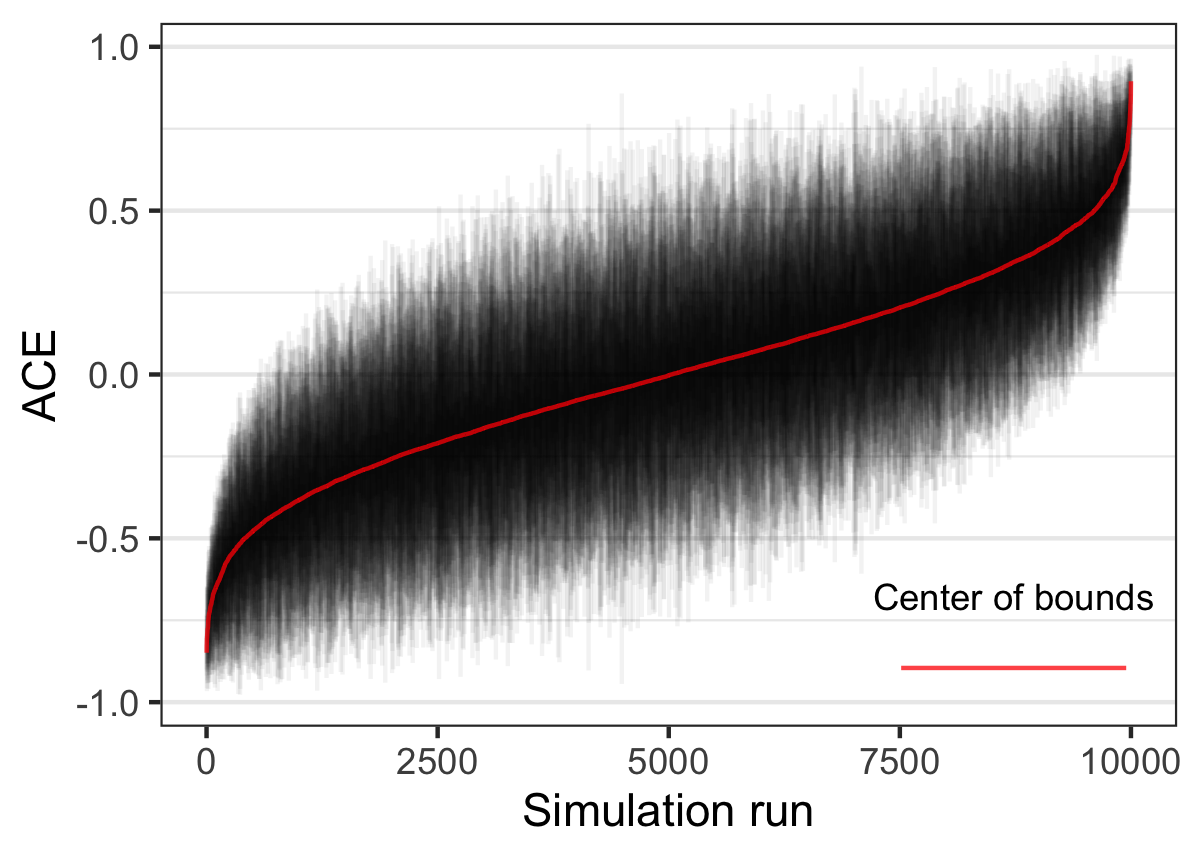
\includegraphics[width=\textwidth]{/Users/ralphtrane/Documents/RPackages_dev/ACEBounds/figures/all_bivariate_bounds.png}
    \caption{Bounds ordered by the center of the bounds.}
    \label{fig:all_biv_bounds}
  \end{subfigure}%
  ~
  \begin{subfigure}[t]{0.5\textwidth}
    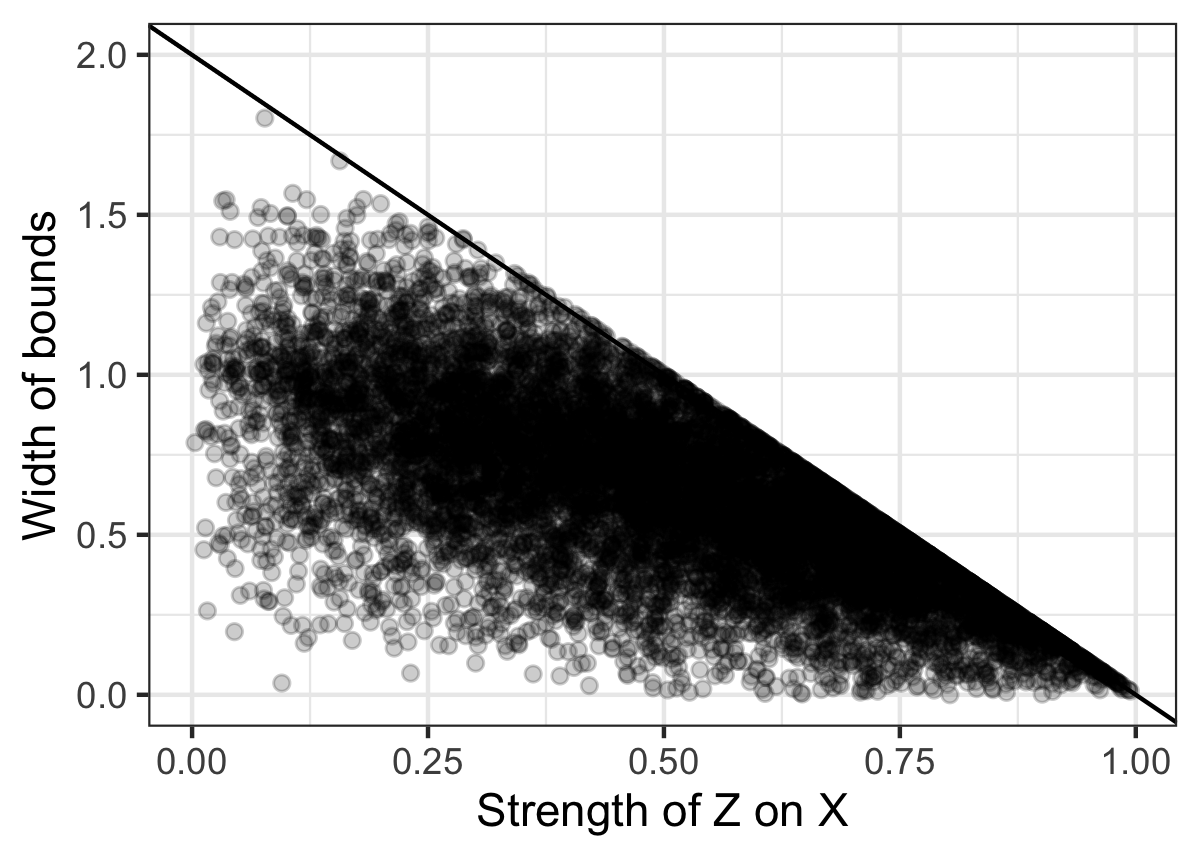
\includegraphics[width=\textwidth]{/Users/ralphtrane/Documents/RPackages_dev/ACEBounds/figures/bivariate_width_vs_strength.png}
    \caption{Black line has intercept 2 and slope -2.}
    \label{fig:biv_width_vs_strength}
  \end{subfigure}
  \caption{10,000 values for bivariate distributions were randomly generated such that no constraints were violated. Of these, 123 resulted in bounds where the lower bound was greater than the upper bounds. These have been removed from these plots.}
  \label{fig:biv_bounds_vs_strength}
\end{figure*}

Figure \ref{fig:all_biv_bounds} shows all bounds sorted by the center of the bounds. What is interesting about this figure is that the entire interval -1 to 1 is covered, and the widths of the bounds vary quite a bit. In many cases, we do indeed see widths greater than 1. It is important to note that the center of the bounds carry no real significance in this context, but is simply used to sort these bounds for illustrative purposes.

Figure \ref{fig:biv_width_vs_strength} shows the widths of the same \(9,877\) bounds plotted against the strength of the instruments. The black line overlayed the plot has intercept 2 and slope -2, which is the upper bound for the width found when including the two monotonicity assumptions. Here we see that this upper bound might very well hold even when we do not include these two assumptions. Here, it is even more evident that a width exceeding 1 is not uncommon.

In Table \ref{tab:prop_of_biv_widths_large}, we see the proportion of the intervals presented on Figure \ref{fig:biv_bounds_vs_strength} with width greater than 1, 0.75, and 0.5, stratified by strength. This shows that while not guaranteed, it is not impossible to observe bounds with width less than 1. However, for IVs with strength less than 0.05, \(47\%\) of the distributions lead to widths greater than 1, and about \(46\%\) of bounds from IVs with strength between \(0.05\) and \(0.1\) have width greater than 1. On the other end of the scale, only \(63\%\) of bounds from IVs with strength greater than \(0.5\) have widths less than \(0.5\).

\begin{table}[H]
  \begin{center}
  \caption{Proportion of bounds from distributions where width is greater than $1$, $0.75$, and $0.5$ stratified by strength of the instrument $Z$ on the exposure $X$.}
  \label{tab:prop_of_biv_widths_large}
  
\begin{tabular}{lccc}
\toprule
\multicolumn{1}{c}{ } & \multicolumn{3}{c}{\makecell[c]{Proportion of bounds with\\ width greater than...}} \\
\cmidrule(l{3pt}r{3pt}){2-4}
Strength & 1 & 0.75 & 0.5\\
\midrule
$[0,0.05]$ & $0.4698795$ & $0.7831325$ & $0.8915663$\\
$(0.05,0.1]$ & $0.4611111$ & $0.7222222$ & $0.8944444$\\
$(0.1,0.25]$ & $0.3227061$ & $0.7029549$ & $0.9222395$\\
$(0.25,0.5]$ & $0.1359280$ & $0.4954981$ & $0.8356085$\\
$(0.5,1]$ & $0.0000000$ & $0.0738818$ & $0.3708067$\\
\bottomrule
\end{tabular}


  \end{center}
\end{table}

In the context of MR analyses, this is a rather depressing result. Most IVs encountered in MR analyses are very weak, which means that the chances that bivariate bounds from MR analyses are informative with width less than 1 are very slim. It should also be noted that while a set of bounds with width greater than 1 provides basically no information, a set of bounds with width just below 1 does not provide much more information. Due to the non-parametric nature of the bounds, the interval \([-0.1, 0.8]\) does not indicate that the average treatment effect is more likely to be positive than the interval \([-0.7, 0.2]\).

\hypertarget{improving-bounds-with-multiple-ivs}{%
\section{Improving Bounds With Multiple IVs}\label{improving-bounds-with-multiple-ivs}}

In Section \ref{properties-of-bounds-from-summary-level-data}, we found that non-parametric bounds derived from bivariate data require rather strong instrumental variables to guarantee useful results. It seems that there simply is not enough information in bivariate data. One natural question is to ask is whether we can aggregate the information from multiple instrumental variables to obtain a set of improved bounds. In this section, we will consider one approach to do just that, and try to characterize what gains can be expected.

To maintain the close connection to MR analyses, we will consider a logistic model that is often used in MR analyses. Specifically, let

\[\begin{aligned}
\text{logit}(P(X = 1 | Z_1 = z_1, ..., Z_n = z_n)) &= \beta_0 + \sum_i \beta_i z_i \\
\text{logit}(P(Y = 1 | X = x)) &= \gamma_0 + \gamma_1 x,
\end{aligned}\]

where \(\text{logit}(a) = \frac{1}{1 + \exp(-a)}\), \(y \in \{0,1\}, x \in \{0,1\}\), \(z_i \in \{0, 1, 2\}\), and \(\beta_i, \gamma_j \in \mathbb{R}\). This particular model is often used in GWAS studies that focus on associations between genetic variants and binary phenotypes (for example, a quick search of the GWAS Central (Beck, Shorter, and Brookes 2020) for ``logistic regression'' returns 177 hits \textbf{NOTE: MANY OF THE ARTICLES ASSOCIATED WITH THESE DO NOT MENTION LOG REG IN METHODS.}). Furthermore, \(P(Z_j = 0) = P(Z_j = 2) = 0.25\) and \(P(Z_j = 1) = 0.5\), which is in line with what would be expected in a Mendelian randomization scenario where pairs of binary alleles are randomly chosen. Here, we will use \(\gamma_0 = -2, \gamma_1 = 0.2\).

To avoid any unpleasant surprises due to randomness from simulating actual data, we decided to integrate (either exactly or numerically depending on the value of \(n\)) to find the probabilities \(P(Y = 1 | Z_j = z_j)\) and \(P(X = 1 | Z_j = z_j)\). We draw the coefficients \(\beta_i \sim \text{Uniform}(0, 1/n)\). This is a scenario similar to what we encounter in the MR setting. Figure \ref{fig:bounds_vs_strength_many_IVs_varying_betas} shows the resulting bounds for the three different values of \(n\) plotted against the strengths of the IVs.

\begin{figure}[H]
  \center
  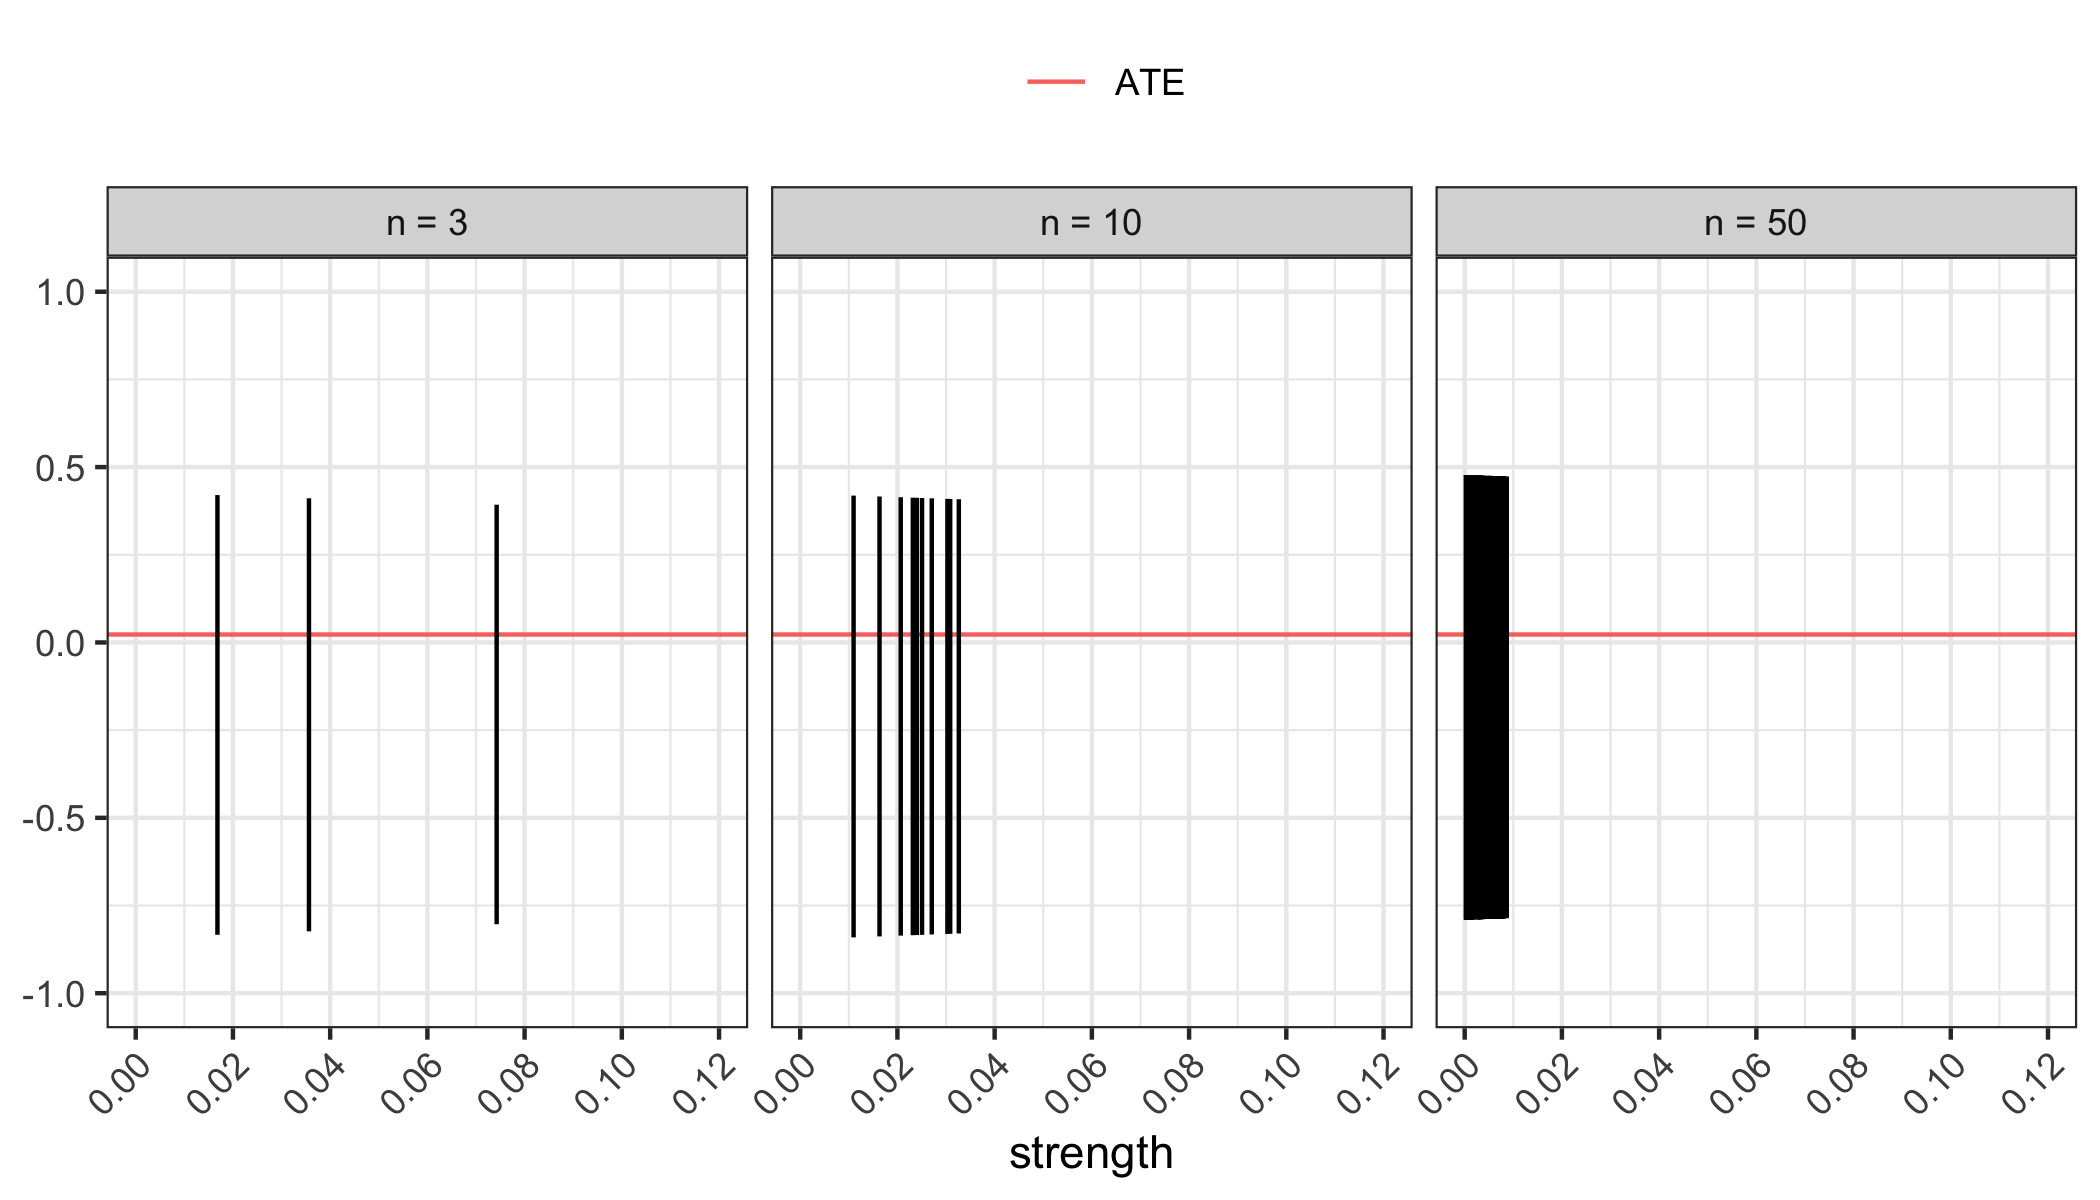
\includegraphics[width = .99\linewidth]{/Users/ralphtrane/Documents/RPackages_dev/ACEBounds/figures/varying_betas_bounds_vs_strength_no_mono.png}
  \caption{Bounds based on probabilities derived from the logistic model. Here, the coefficients are randomly chosen as $\text{Uniform}(0, 1/n)$ for different values of $n$.}  
  \label{fig:bounds_vs_strength_many_IVs_varying_betas}
\end{figure}

Figure \ref{fig:bounds_vs_strength_many_IVs_varying_betas} shows that when many valid IVs are present, the individual bivariate upper and lower bounds seems to be monotonically decreasing and increasing, respectively, as the strength of the IV increases. This means intersections of intervals from many IVs will result in an interval very similar, if not identical, to the most narrow of the individual bounds, which in turn will be the interval derived using the strongest of the IVs.

Another interesting, although not surprising, observation is the shrinking of the strengths of the indiviudal instruments when the total number of instruments increases. With many instruments, the linear combination \(\beta_0 + \sum_i \beta_i z_i\) will generally be relatively large, simply by chance. This means that the effect on \(P(X = 1 | Z_1, ..., Z_n)\) of a single instrument being 1 instead of 0 is quite small. This is important. In Section \ref{bounds-from-bivariate-data}, we saw that chances of obtaining informative bounds with weak instruments are slim. If one believes the true model includes many instruments, chances are that these are relatively weak.

In MR analyses based on bivariate data from GWAS results, this indicates that aggregating information from multiple instruments in a simple manor, such as taking interceptions, will not result in more information than simply using the best of the individual bounds. This strategy is only appropriate in a situation where all the proposed instruments are valid. If we on the other hand want to protect ourselves against using bounds from a potentially invalid instrument by taking the union of the bounds from many proposed instruments, we would end up with very conservative bounds. This would in turn provide even less information about the ATE. This is partly due to the lack of guarantees on the width of the bounds obtained from bivariate data (Section \ref{bounds-from-bivariate-data}), which means it is very unlikely that a collection of instruments all provide informative bounds. When combining bounds through unions, only attributes shared among all bounds will be preserved, so if just one weak instrument is included, the resulting union bounds will provide very little information.

\hypertarget{what-can-you-do-with-summary-level-data-for-bounds-a-quasi-bayesian-path-to-more-information}{%
\section{What can you do with summary-level data for bounds? A Quasi-Bayesian Path to More Information}\label{what-can-you-do-with-summary-level-data-for-bounds-a-quasi-bayesian-path-to-more-information}}

\label{quasi-bayesian}

Although bivariate data does not provide enough information for the derived bounds to guarantee the same desirable and useful qualities as their trivariate counterparts, they still provide some information about the trivariate data distribution. In this section, we will demonstrate a simple approach to use the bivariate data to describe the set of possible trivariate distributions, and their bounds.

The idea is relatively simple: we wish to use the known quantities \(P(X = x | Z = z)\) and \(P(Y = y | Z = z)\) to get a sense of which possible distributions \(P(X = x, Y = y | Z = z)\) marginalize to the known distributions, while satisfying the constraints obtained from the polymake program. By repeatedly, and independently, drawing such trivariate distributions, we can get a sense of the bounds trivariate data could give. Using this, questions about the potential information one could gain from knowing the full trivariate distribution can be answered.

\hypertarget{sampling-procedure}{%
\subsection{Sampling Procedure}\label{sampling-procedure}}

The joint conditional distribution \(P(X = x, Y = y | Z = z)\) can be constructed from the marginal conditional distributions \(P(X = x | Z = z)\) and \(P(Y = y | Z = z)\) if we know the values of \(\text{Cov}(X, Y | Z = z)\) for each \(z\), since

\begin{equation}
P(X = x, Y = y | Z = z) = P(X = x | Z = z)P(Y = y | Z = z) + (2\cdot I[x = y] - 1)\text{Cov}(X, Y | Z = z). \label{eq:cov-expression}
\end{equation}

Since these covariances are essentially completely unknown to us, we draw them uniformly from the set of values that result in the joint conditional distribution of \((X,Y|Z)\) being an actual probability distribution satisfying the verifiable constraints from \eqref{eq:constraints}.

This set of values is not trivial, but fortunately we can find a superset of values that is much smaller than \([-1,1]^k\). When implementing this approach, we propose a set of covariances by sampling from this superset, construct the trivariate distribution, and check if any constraints are violated. If there are any violations, the proposed set of covariances is discarded, and a new set proposed.

Combining \(0 \le P(X = x, Y = y | Z = z) \le 1\) for all values of \(z = 0, 1, ..., k-1\) with \eqref{eq:cov-expression}, we see that

\begin{equation*}
-P(X = x | Z = z) P(Y = y | Z = z) \le \text{Cov}(X, Y | Z = z) \le 1 - P(X = x | Z = z)P(Y = y | Z = z)
\end{equation*}

when \(x = y\), and

\begin{equation*}
P(X = x | Z = z) P(Y = y | Z = z) - 1 \le \text{Cov}(X, Y | Z = z) \le P(X = x | Z = z)P(Y = y | Z = z)
\end{equation*}

when \(x \neq y\). Since this holds for all \(z = 0,1,...,k-1\), we find that \(\text{Cov}(X, Y | Z = z)\) must be such that

\[
\begin{aligned}
  \max_z\left\{ 
      \begin{array}{c}
        -P(X = 1 | Z = z)P(Y = 1 | Z = z) \\
        -P(X = 0 | Z = z)P(Y = 0 | Z = z) \\ 
        P(X = 1 | Z = z)P(Y = 0 | Z = z) - 1\\
        P(X = 0 | Z = z)P(Y = 1 | Z = z) - 1
      \end{array} 
    \right\} & \\ 
    \le \text{Cov}(X, &Y | Z = z) \le \\
    &\min_z\left\{ 
      \begin{array}{c}
        1 - P(X = 1 | Z = z)P(Y = 1 | Z = z) \\
        1 - P(X = 0 | Z = z)P(Y = 0 | Z = z) \\ 
        P(X = 1 | Z = z)P(Y = 0 | Z = z) \\
        P(X = 0 | Z = z)P(Y = 1 | Z = z)
      \end{array} 
    \right\}
\end{aligned}
\]

Furthermore, enforcing the IV inequalities \(\max_x \sum_y \max_z P(X = x, Y = y | Z = z) \le 1\), we get constraints on the differences between \(\text{Cov}(X, Y | Z = z_1)\) and \(\text{Cov}(X, Y | Z = z_2)\). For any \(x=0,1\), and any pair \((z_1, z_2) \in \{0,1,...,k-1\} \times \{0,1,...,k-1\}\), we see that \(0 \le P(X = x, Y = 0 | Z = z_1) + P(X = x, Y = 1 | Z = z_2) \le 1\) (where the first inequality is a result of summing two positive quantities). From \eqref{eq:cov-expression}, we also see that for \(x=0\),

\[
\begin{aligned}
0 \le & \\ 
& P(X = 0 | Z = z_1)P(Y = 0 | Z = z_1) + \text{Cov}(X, Y | Z = z_1) + P(X = 0 | Z = z)P(Y = 1 | Z = z_2) - \text{Cov}(X, Y | Z = z_2) \\ 
& \le 1,
\end{aligned}
\]

which is equivalent to

\[
\begin{aligned}
-P(X = 0 | Z = z_1)P(Y = 0 | &Z = z_1) - P(X = 0 | Z = z)P(Y = 1 | Z = z_2) \\
\le \text{Cov}(X, Y | Z = z_1) &- \text{Cov}(X, Y | Z = z_2) \le \\
1 - P(X = 0 | &Z = z_1)P(Y = 0 | Z = z_1) - P(X = 0 | Z = z)P(Y = 1 | Z = z_2).
\end{aligned}
\]

A similar exercise can be done for \(x = 1\). The result is that, for any pair of \((z_1, z_2) \in \{0,1,...,k-1\} \times \{0,1,...,k-1\}\), the values of \(\text{Cov}(X, Y | Z = z_1)\) and \(\text{Cov}(X, Y | Z = z_1)\) must satisfy

\[
\begin{aligned}
  \max\left\{ 
      \begin{array}{c}
        -P(X = 0 | Z = z_1)P(Y = 0 | Z = z_1) - P(X = 0 | Z = z_2)P(Y = 1 | Z = z_2) \\ 
        P(X = 1 | Z = z_1)P(Y = 0 | Z = z_1) + P(X = 1 | Z = z_2)P(Y = 1 | Z = z_2) -1 \\
        P(X = 0 | Z = z_2)P(Y = 0 | Z = z_2) + P(X = 0 | Z = z_1)P(Y = 1 | Z = z_1) - 1 \\
        -P(X = 1 | Z = z_2)P(Y = 0 | Z = z_2) - P(X = 1 | Z = z_1)P(Y = 1 | Z = z_1)
      \end{array} 
    \right\} \qquad \qquad & \\ \\
    \le \text{Cov}(X,Y | Z = z_1) - \text{Cov}(X,Y | Z = z_2) \le \qquad \qquad \qquad \qquad  \qquad& \\ \\
    \min\left\{ 
      \begin{array}{c}
        1 -P(X = 0 | Z = z_1)P(Y = 0 | Z = z_1) - P(X = 0 | Z = z_2)P(Y = 1 | Z = z_2) \\ 
        P(X = 1 | Z = z_1)P(Y = 0 | Z = z_1) + P(X = 1 | Z = z_2)P(Y = 1 | Z = z_2) \\
        P(X = 0 | Z = z_2)P(Y = 0 | Z = z_2) + P(X = 0 | Z = z_1)P(Y = 1 | Z = z_1) \\
        1 - P(X = 1 | Z = z_2)P(Y = 0 | Z = z_2) - P(X = 1 | Z = z_1)P(Y = 1 | Z = z_1)
      \end{array} 
    \right\} & 
\end{aligned}
\]

To create a possible set of values of \(P(X = x, Y = y | Z = z)\), we sequentially draw values for \(\text{Cov}(X, Y | Z = 0), \text{Cov}(X, Y | Z = 1), ..., \text{Cov}(X, Y | Z = k-1)\), such that the above inequalities hold, calculate the values of \(P(X = x, Y = y | Z = z)\) using \eqref{eq:cov-expression}, and check that the constraints in \eqref{eq:constraints} are satisfied. If any of the constraints are violated, the values are rejected, and the procedure repeated until we have a set of values for \(\text{Cov}(X, Y | Z = 0), \text{Cov}(X, Y | Z = 1), ..., \text{Cov}(X, Y | Z = k-1)\) that result in a trivariate probability distribution that satisfies the constraints in \eqref{eq:constraints}.

The ultimate goal of this exercise is to try to assess whether knowledge about the full trivariate probabilities would allow us to determine direction of the ATE. In most cases there is not a firm answer to this question, as some trivariate probabilities result in bounds that would, while other trivariate probability distributions result in bounds that would not. So, we are really trying to asses questions such as ``given the bivariate probabilities, what is the chance that the trivariate data would allow us to determine direction?''

The approach presented here can, under the right set of assumptions, be interpreted as generating a sample from the posterior distribution over all possible trivariate distributions given the marginalized probabilities, and a uniform prior on the unknown quantities \(\text{Cov}(X, Y | Z = z)\). This means that we can obtain posterior probabilities of certain events. In particular, we will be interested in the posterior probability that the trivariate bounds contain \(0\). We will use this as a heuristic measure of the loss of information in going from trivariate to bivariate data.

\hypertarget{single-iv-case}{%
\subsection{Single IV Case}\label{single-iv-case}}

To illustrate the method described in the previous section, we start by considering the single IV case. This allows us to easily explore the behavior of this method, and present a few different scenarios. In Section \ref{multiple-iv-case}, we describe how this method can be used if multiple instruments are available.

Depending on the values of \(P(X = 1 | X = z)\) and \(P(Y = 1 | Z = z)\), the picture this approach paints can vary dramatically, which in turn leads to very different conclusions. Here, we will consider nine different sets of values of these marginal distributions that illustrate a few different scenarios one can end up in when using this quasi-bayesian approach. The marginal distributions are presented in Table \ref{tab:subset_plot_summaries_b} below, while Table \ref{tab:subset_plot_summaries_a} shows the estimated posterior probability of the trivariate bounds containing \(0\) based on 1000 trivariate distributions sampled as described in Section \ref{sampling-procedure}. All trivariate bounds are shown on Figure \ref{fig:trivariate_bounds}.

\begin{table}[H]
  \center
  \caption{Values of $P(X = 1 | Z = z)$ and $P(Y = 1 | Z = z)$ used to illustrate our quasi-bayesian approach. These are presented with $\{P(X = 1 | Z = 0), P(X = 1 | Z = 1), P(X = 1 | Z = 2)\}$ on the first row, and $\{P(Y = 1 | Z = 0), P(Y = 1 | Z = 1), P(Y = 1 | Z = 2)\}$ on the second row.}
  \label{tab:subset_plot_summaries_b}
  
\begin{tabular}{llll}
\toprule
  & Column 1 & Column 2 & Column 3\\
\midrule
Row a & \makecell[l]{\{0.125, 0.399, 0.080\}\\\{0.699, 0.840, 0.742\}} & \makecell[c]{\{0.244, 0.275, 0.185\}\\\{0.238, 0.089, 0.146\}} & \makecell[r]{\{0.603, 0.469, 0.310\}\\\{0.638, 0.346, 0.719\}}\\
Row b & \makecell[l]{\{0.886, 0.968, 0.874\}\\\{0.805, 0.822, 0.951\}} & \makecell[c]{\{0.139, 0.441, 0.334\}\\\{0.179, 0.359, 0.559\}} & \makecell[r]{\{0.901, 0.909, 0.935\}\\\{0.821, 0.810, 0.905\}}\\
Row c & \makecell[l]{\{0.175, 0.079, 0.365\}\\\{0.599, 0.358, 0.087\}} & \makecell[c]{\{0.493, 0.911, 0.085\}\\\{0.360, 0.480, 0.441\}} & \makecell[r]{\{0.434, 0.045, 0.733\}\\\{0.747, 0.370, 0.169\}}\\
\bottomrule
\end{tabular}


\end{table}

\begin{table}[H]
  \center
  \caption{For each of the nine panels displayed in figure \ref{fig:trivariate_bounds}, this table includes lower and upper bounds based on the bivariate data, and proportion of trivariate distributions overlapping 0.}
  \label{tab:subset_plot_summaries_a}
  
\begin{tabular}{llll}
\toprule
  & Column 1 & Column 2 & Column 3\\
\midrule
Row a & \makecell[l]{[-0.583, 0.338]\\100.00\%} & \makecell[c]{[-0.331, 0.814]\\76.00\%} & \makecell[r]{[-0.574, 0.468]\\63.20\%}\\
Row b & \makecell[l]{[-0.156, 0.758]\\100.00\%} & \makecell[c]{[-0.077, 0.693]\\11.00\%} & \makecell[r]{[-0.129, 0.897]\\98.00\%}\\
Row c & \makecell[l]{[-0.275, 0.24]\\100.00\%} & \makecell[c]{[-0.136, 0.214]\\88.30\%} & \makecell[r]{[-0.083, 0.112]\\41.00\%}\\
\bottomrule
\end{tabular}


\end{table}

\begin{figure}[H]
  \center
  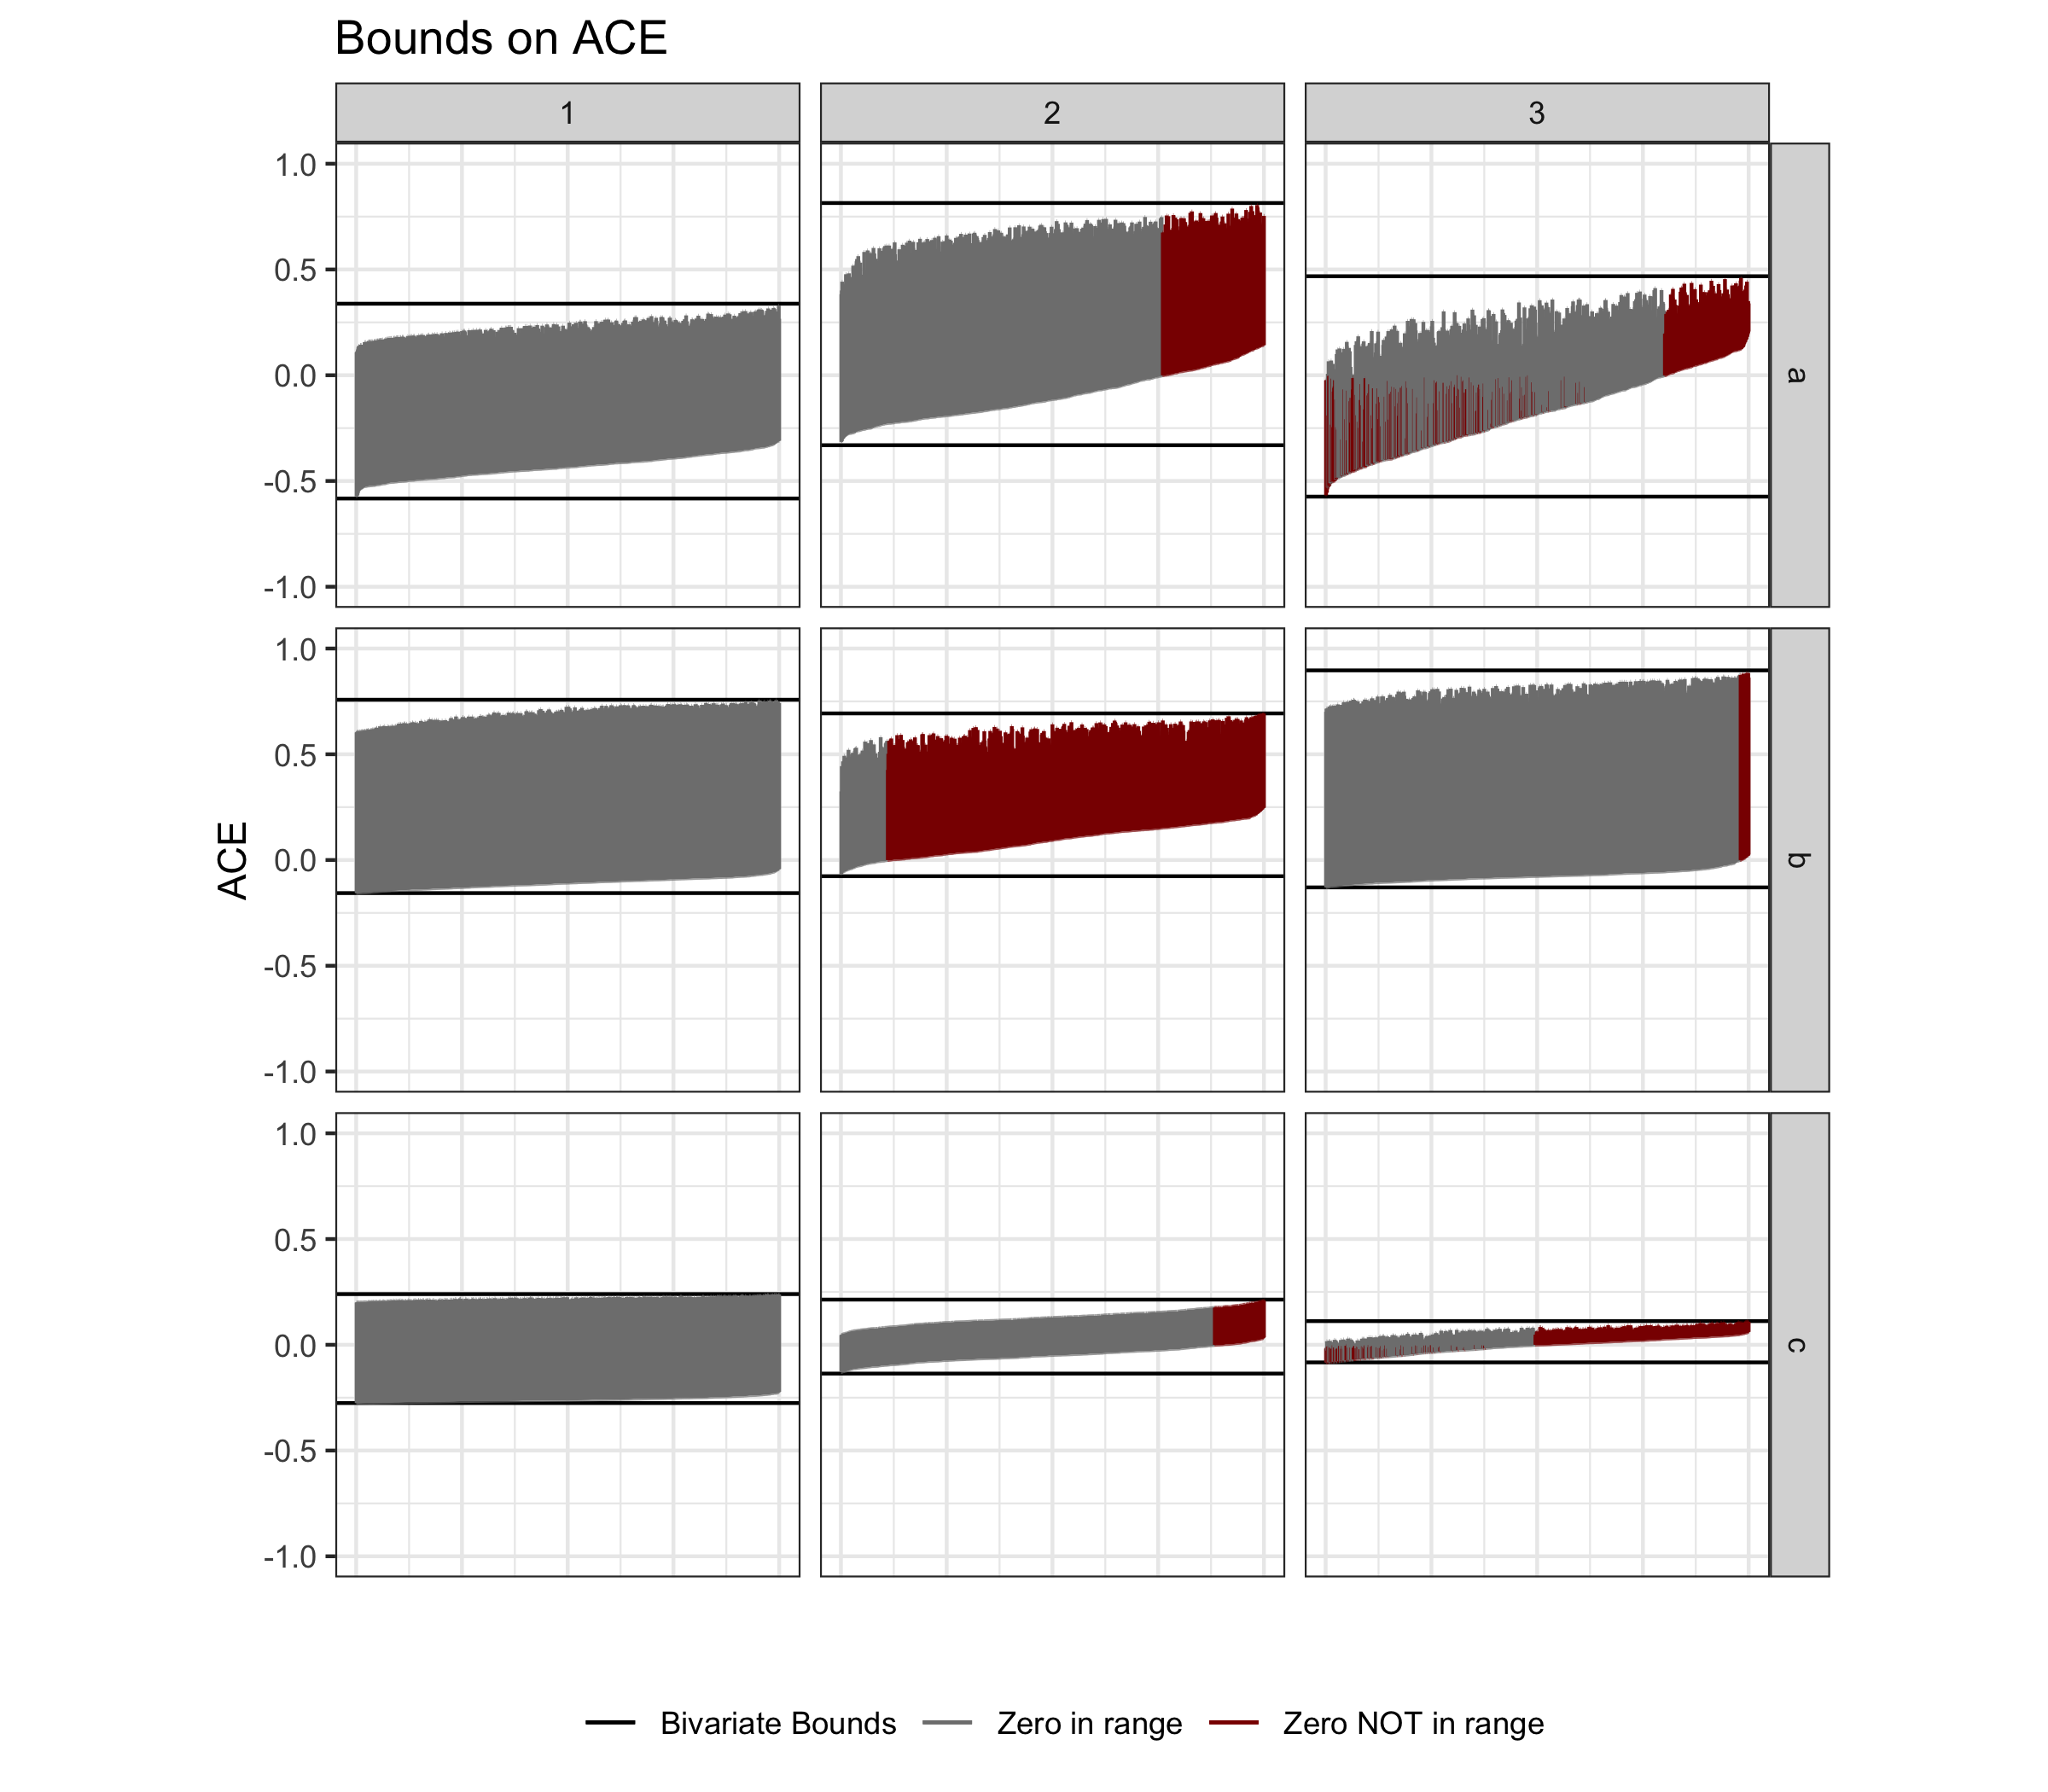
\includegraphics[width=\linewidth]{/Users/ralphtrane/Documents/RPackages_dev/ACEBounds/figures/trivariate_bounds_subset_plot.png}
  \caption{Trivariate bounds are constructed from the bivariate distribution by drawing values for $\text{Cov}(X,Y|Z=z),z=0,1,2$. Even similar bivariate distributions can result in very different insights.}
  \label{fig:trivariate_bounds}
\end{figure}

Row a shows three scenarios where the bivariate bounds are all more or less centered around zero with similar widths. However, the conclusions are rather different. Column 1 shows no trivariate distribution would allow us to determine the direction of the ATE using bounds. Column 2 indicates that about 24\% of the possible trivariate distributions would allow us to determine direction, while for column 3 that number is approximately 36.8\%. However, while the direction is always the same for column 2 (positive), it varies for column 3.

Row b illustrates three scenarios where the bivariate bounds are centered well above zero, and all of similar large widths. Here, we see one case where we have no hope of determining direction from trivariate bounds (column 1), one case where we are most likely to be able to determine the direction of the ATE to be positive from trivariate bounds (column 2), and one case where we are rather unlikely to be able to determine the direction of the ATE from trivariate bounds (column 3).

Row c is similar to row a in that all bivariate bounds are centered around 0, but here all bivariate bounds are rather narrow. The three columns indicate similar conclusions as seen in row a. This shows that even with rather narrow bivariate bounds centered around 0, the intuitive idea that trivariate bounds would not be able to detect direction is misguided.

The diverse conclusions from relatively similar bivariate bounds indicate that there is no simple way to determine whether trivariate bounds would be useful from just the bivariate bounds. Even very different marginal distributions at times result in similar conclusions about the usefulness of trivariate bounds, and vice versa.

It is important to reflect on the interpretation of these posterior probabilities. A scenario like the one resulting in the bounds presented in row b, column 2 only provides information about the trivariate bounds under the assumption that all possible valid trivariate probability distributions are equally likely. Under this assumption, it tells us that it is much more likely that the ATE is positive. It does not, however, rule out a negative value of the ATE. What it does tell us is that trivariate bounds will not be able to determine direction \emph{if the ATE is in fact negative}. This conclusion only hinges on the correctness of the marginal probabilities, \(P(X = 1 | Z = z)\) and \(P(Y = 1 | Z = z)\), and the assumptions presented in Section \ref{iv-assumptions-and-two-sample-mr}.

\hypertarget{multiple-iv-case}{%
\subsection{Multiple IV Case}\label{multiple-iv-case}}

Although the bivariate bounds often do not provide much information themselves, as we saw in the previous section, the little information available can sometimes provide some insights. The approach presented draws on the fact that trivariate bounds are guaranteed to be much narrower than bivariate bounds. It remains to be seen if utilizing such an approach while aggregating information from multiple IVs through intersections of bounds can be useful.

The simplest extension to the multiple IV scenario, is to simply repeat the sampling procedure presented in Section \ref{sampling-procedure} for each proposed instrument before creating the combined bounds by taking the intersection of the pairwise bounds. This builds on one main assumption in that the two sampling procedures are done independently, and so implicitly assume that the covariances of \(X\) and \(Y\) given \(Z_1\) are independent of the covariances of \(X\) and \(Y\) given \(Z_2\).

Specifically, say we get bounds \((LB_{1i},UB_{1i}),i = 1,2,...,m\) by sampling m trivariate distributions based on the information we have on \((X,Z_1)\) and \((Y,Z_1)\), and bounds \((LB_{2i}, UB_{2i}),i = 1,2,...,m\) by sampling \(m\) trivariate distributions based on the information we have on \((X,Z_2)\) and \((Y,Z_2)\). We then create the intersection bounds as \(\left(\max_{z \in {1,2}} LB_{zi}, \min_{z \in {1,2}} UB_{zi}\right), i = 1, 2, ..., m\). This, under the assumption that \(\text{Cov}(X, Y | Z_1 = z)\) and \(\text{Cov}(X, Y | Z_2 = z)\) are independent of each other, gives us a sample from the posterior distribution of intersection bounds. We can use this to assess the potential usefulness of aggregating information from two sets of trivariate data, \((X, Y, Z_1)\) and \((X, Y, Z_2)\), using intersection bounds.

We will illustrate this approach in the next section using data obtained from MRBase.

\hypertarget{data-analysis}{%
\section{Data Analysis}\label{data-analysis}}

In this section we will consider two example analyses demonstrating the approaches presented above. The data was obtained using the IEU GWAS database, which is available in R through the \texttt{TwoSampleMR} package. (Hemani et al. 2018) We will explore the non-parametric bounds obtained from bivariate data sources, and what conclusions are attainable based on our quasi-bayesian approach. To do so, we consider two examples: the effect of smoking on depression, and the effect of smoking on lung cancer.

To be able to find non-parametric bounds, we need estimates of the marginal probabilities \(P(Y = 1 | Z = z)\) and \(P(X = 1 | Z = z)\). To do so, we use the \texttt{TwoSampleMR} R-package. This allows us to find studies that have explored the effects of genetic variants on the exposure and outcome variables we are interested in. Instruments were extracted, and LD based clumping (\(r^2 \ge 0.001\) within a \(10,000\) kb window using \(p < 5 \times 10^{-8}\) as the level of significance) performed such that only independent instruments with significant associations are returned. The data is harmonized to make sure that the effects of the SNPs on exposure and outcome were measured with the same allele as reference. We obtain coefficients from GWAS experiments corresponding to the effects of the SNPs on the exposure, and the outcome from a logistic model. Since no intercept for these models are included in the reported results, but marginal proportions of the outcome, exposure, and allele frequencies are, we find the intercepts by solving \(P(X = 1) = \sum_{z = 0}^2\text{logit}(\beta_0 + \hat{\beta_1}\cdot z)\cdot P(Z = z)\) and \(P(Y = 1) = \sum_{z = 0}^2\text{logit}(\gamma_0 + \hat{\gamma_1}\cdot z)\cdot P(Z_j = z)\) for \(\beta_0\) and \(\gamma_0\), respectively. This allows us to calculate \(P(Y = 1 | Z_j = z)\) and \(P(X = 1 | Z_j = z)\) for every \(j\) and \(z=0,1,2\). With these quantities, non-parametric bounds on the ATE can be calculated.

For complete and reproducible code, see \textbf{{[}link to vignette showing analysis on pkgdown page{]}}.

\hypertarget{smoking-effect-on-depression}{%
\subsection{Smoking effect on depression}\label{smoking-effect-on-depression}}

In our first example, we explore the effect smoking has as an exposure on the outcome depression. It has previously been suggested that smoking increases the risk of depression. Wootton et al. (2019) estimated the odds ratio using an inverse-variance weighted method to be 1.99 with a 95\% confidence interval of {[}1.71, 2.32{]} suggesting a relatively strong causal effect.

Data on \((X|Z)\) is obtained from the experiment with id ukb-d-20116\_0 in the MRBase database, and data on \((Y|Z)\) is obtained from the experiment with id ukb-d-20544\_11. We find 84 genetic variants that can be used as instruments for the effect of smoking on depression. Using these 84 genetic variantes, we want to first explore if non-parametric bounds can be used to obtain any information about the average treatment effect of smoking on the chances of developing depression. We will follow up on this with an exploration of the conclusions our quasi-bayesian approach can provide in this specific example. Finally, we will take a look at intersections of these bounds, and comment on the usefulness of this approach in this practical setting.

The genetic markers that were identified here as potential instruments all look very similar in terms of the estimated conditional distributions of exposure and outcome given instruments. Figure \ref{fig:smoking_on_depression_marginals} shows histograms of the values of \(P(X = 1|Z = z)\) and \(P(Y = 1|Z = z), z = 0,1,2\), for all 84 instruments. As you can see, there is very little variation in the actual values. Especially the small change when moving from \(z = 0\) through \(z = 1\) to \(z = 2\) on the three left panels is of interest here, as this is our first indication that these instruments might be rather weak.

\begin{figure}[H]
  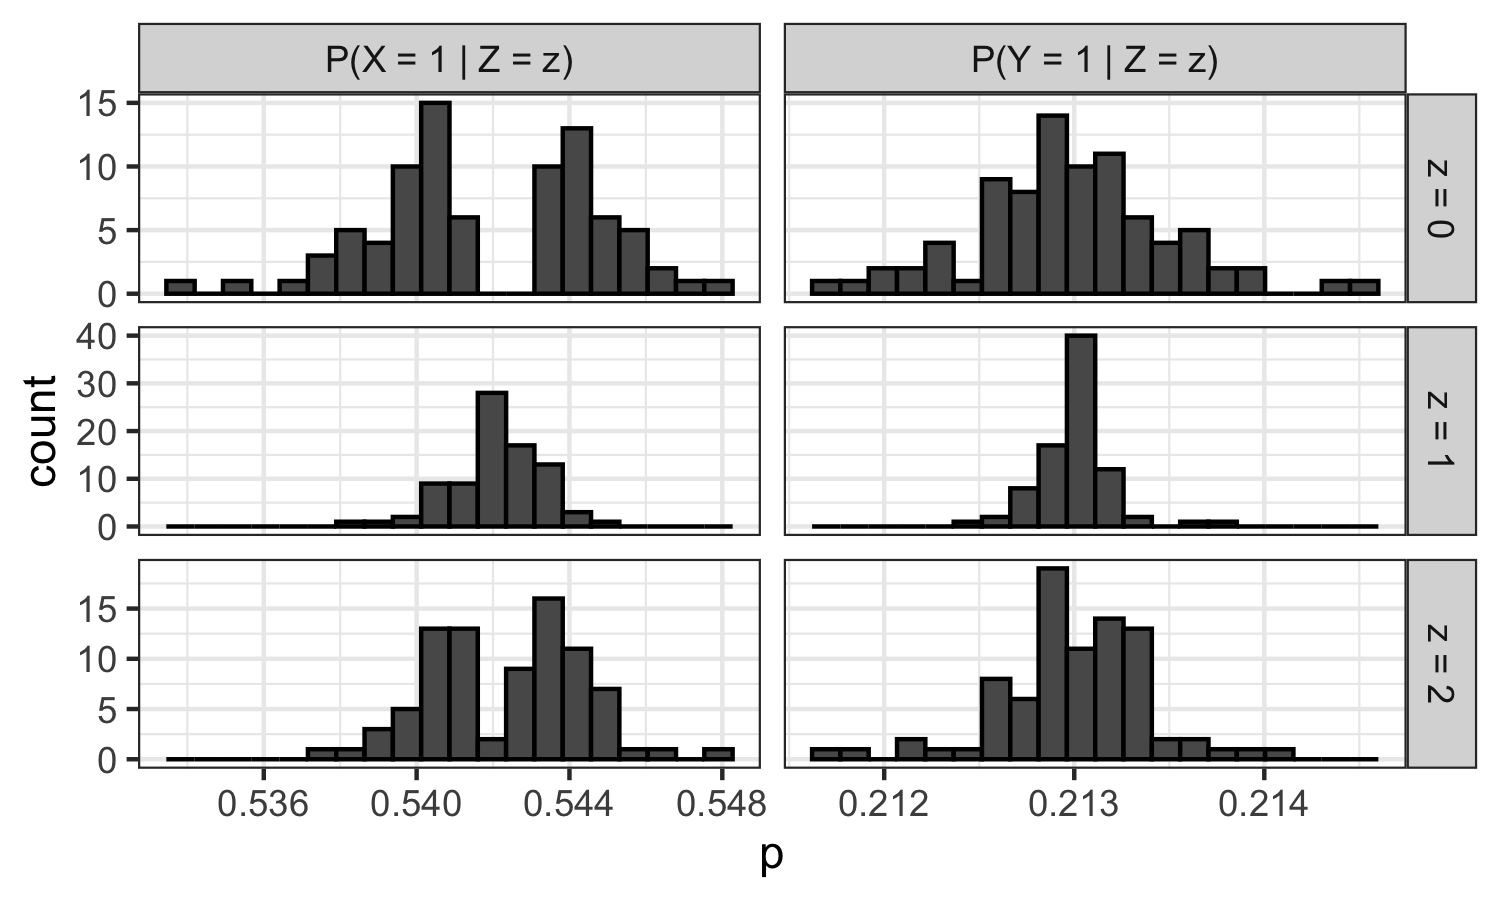
\includegraphics[width = 0.99\linewidth]{/Users/ralphtrane/Documents/RPackages_dev/ACEBounds/figures/example_analyses/smoking_depression_marginal_conditionals.png}
  \caption{Histograms of the marginal conditional probabilities $P(X = 1 | Z = z), z = 0,1,2$ and $P(Y = 1 | Z = z), z=0,1,2$.}
  \label{fig:smoking_on_depression_marginals}
\end{figure}

Figure \ref{fig:strength_histogram} shows a histogram of the strength of all the potential instruments. We see here that the strength of the strongest instrument is less than 0.01, which is much smaller than the 0.5 needed to guarantee narrow bounds, and well in line with the observation on Figure \ref{fig:smoking_on_depression_marginals}. More information on the instruments and summary statistics can be found in Appendix \ref{more-details-data-application-appendix}.

\begin{figure}[H]
  \center
  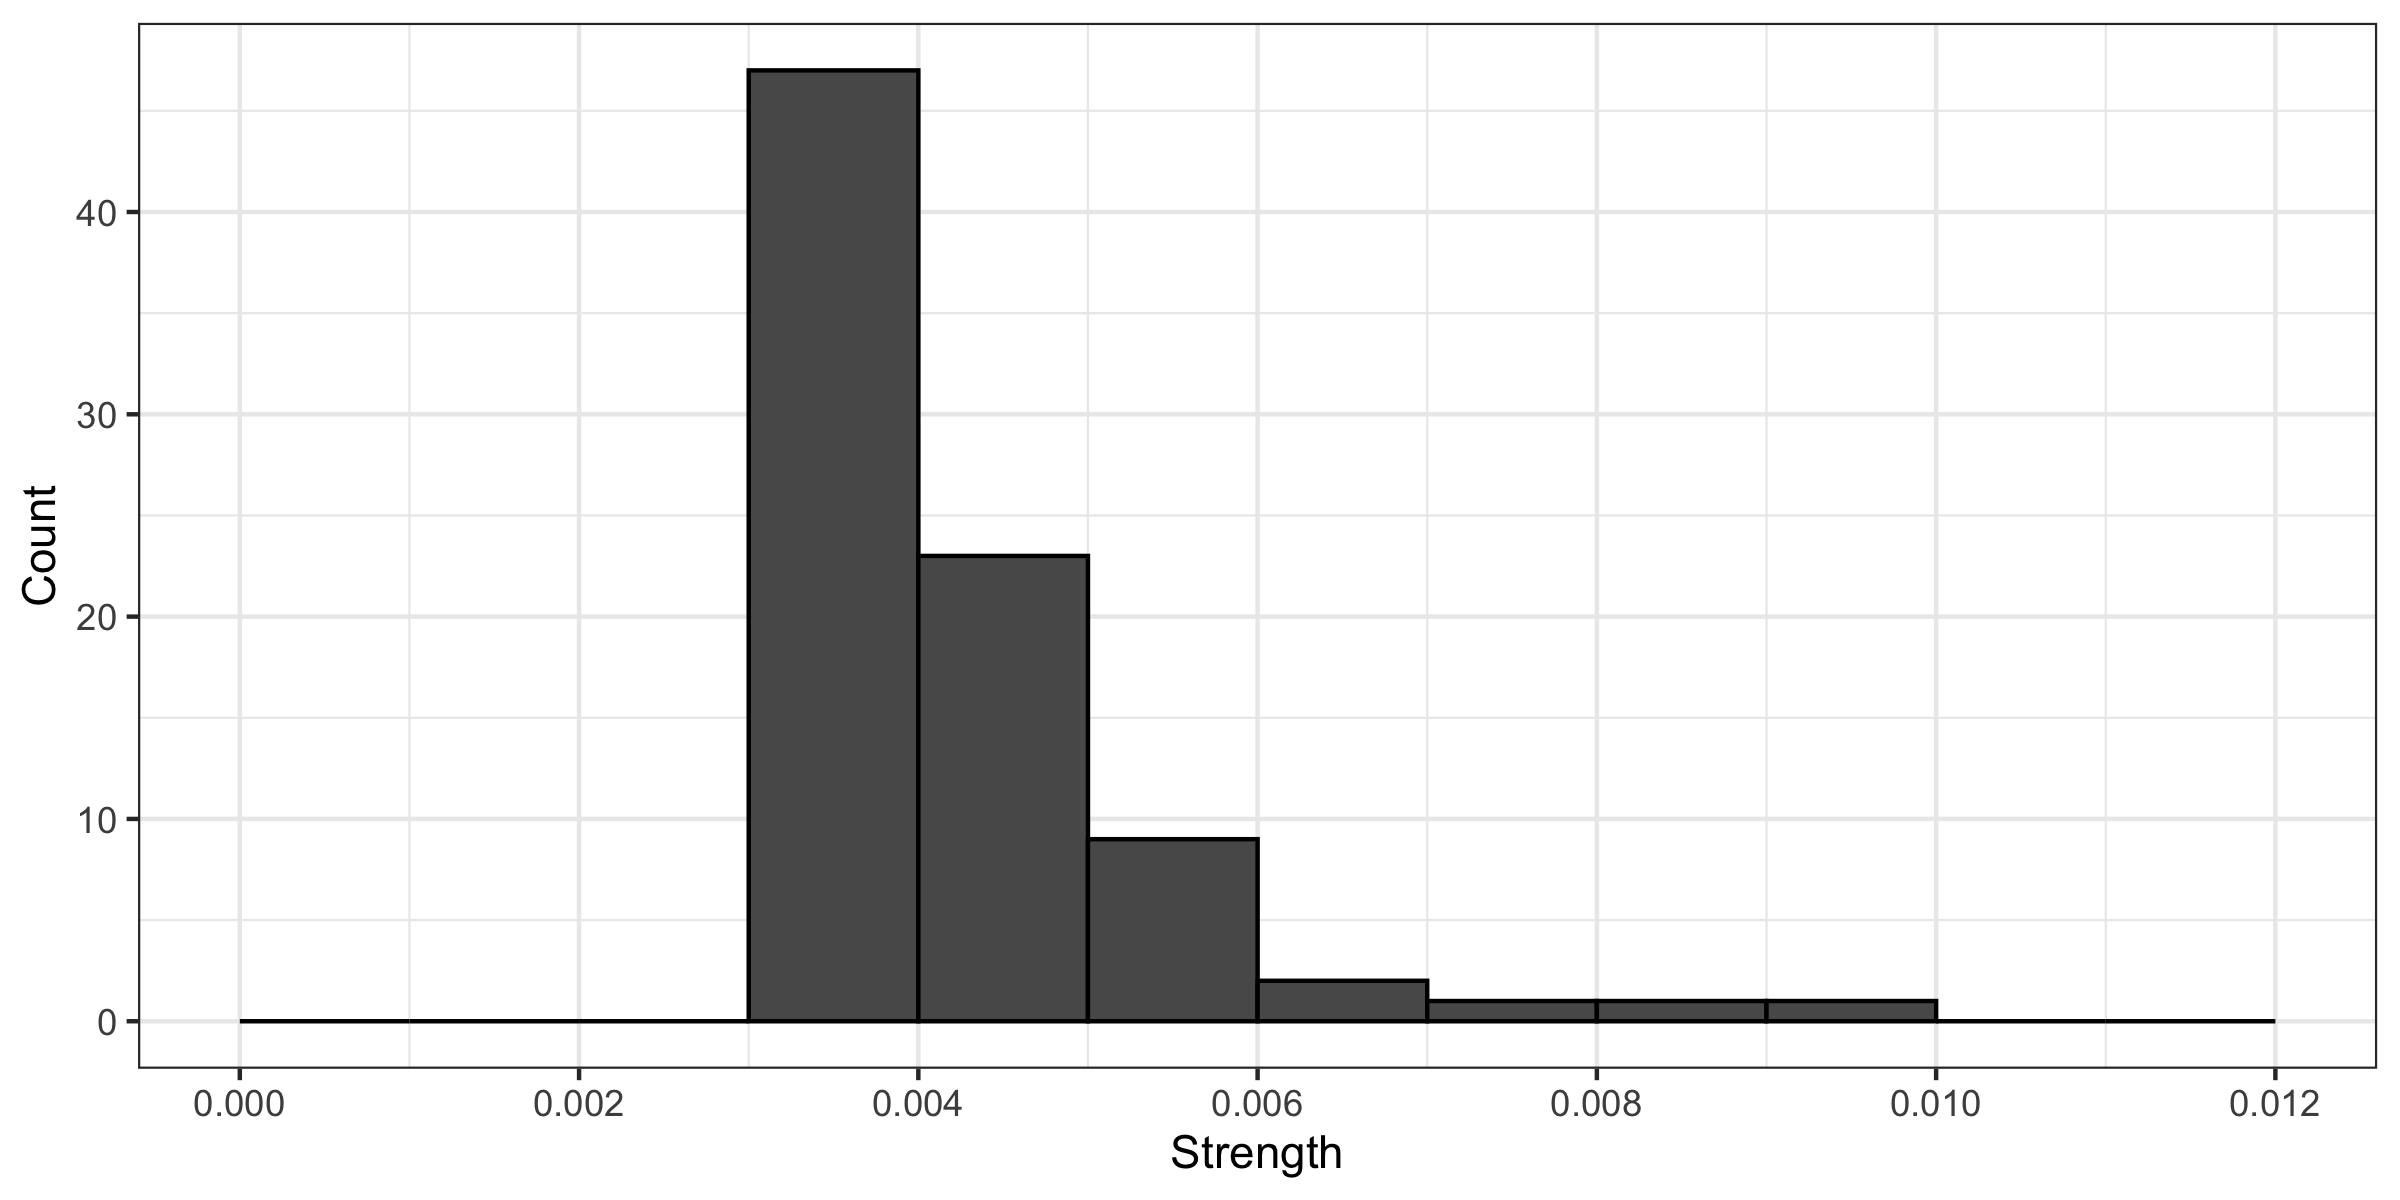
\includegraphics[width = 0.99\linewidth]{/Users/ralphtrane/Documents/RPackages_dev/ACEBounds/figures/example_analyses/strength_histogram.png}
  \caption{Histogram of strengths of IVs on the exposure. Here, SNPs are IVs, and smoking status (ever/never) is exposure. We see that all IVs are very weak, with the largest value just below 0.01.}
  \label{fig:strength_histogram}
\end{figure}

From the 84 instrumental variables found, we obtain 84 sets of bounds using the values of \(P(X = 1 | Z_j = z), P(Y = 1 | Z_j = z), z = 0,1,2,\ j=1,2,...,84\). These are shown on Figure \ref{fig:smoking_on_depression_ind_bounds}. From this figure, it is immediately clear that all the intervals are practically identical. This means that none of these instruments result in bounds that can help us determine direction of the ATE, and, in general, the amount of information they provide on the magnitude of the ATE is limited. This also tells us that trying to aggregate information from these instruments by simply creating intersection bounds will lead to essential no gains.

The very minimal amount of information we get from these bounds is no surprise. As already mentioned, all instruments are very weak, which as we saw in Section 3.1 tend to lead to wide bounds.

\begin{figure}[H]
  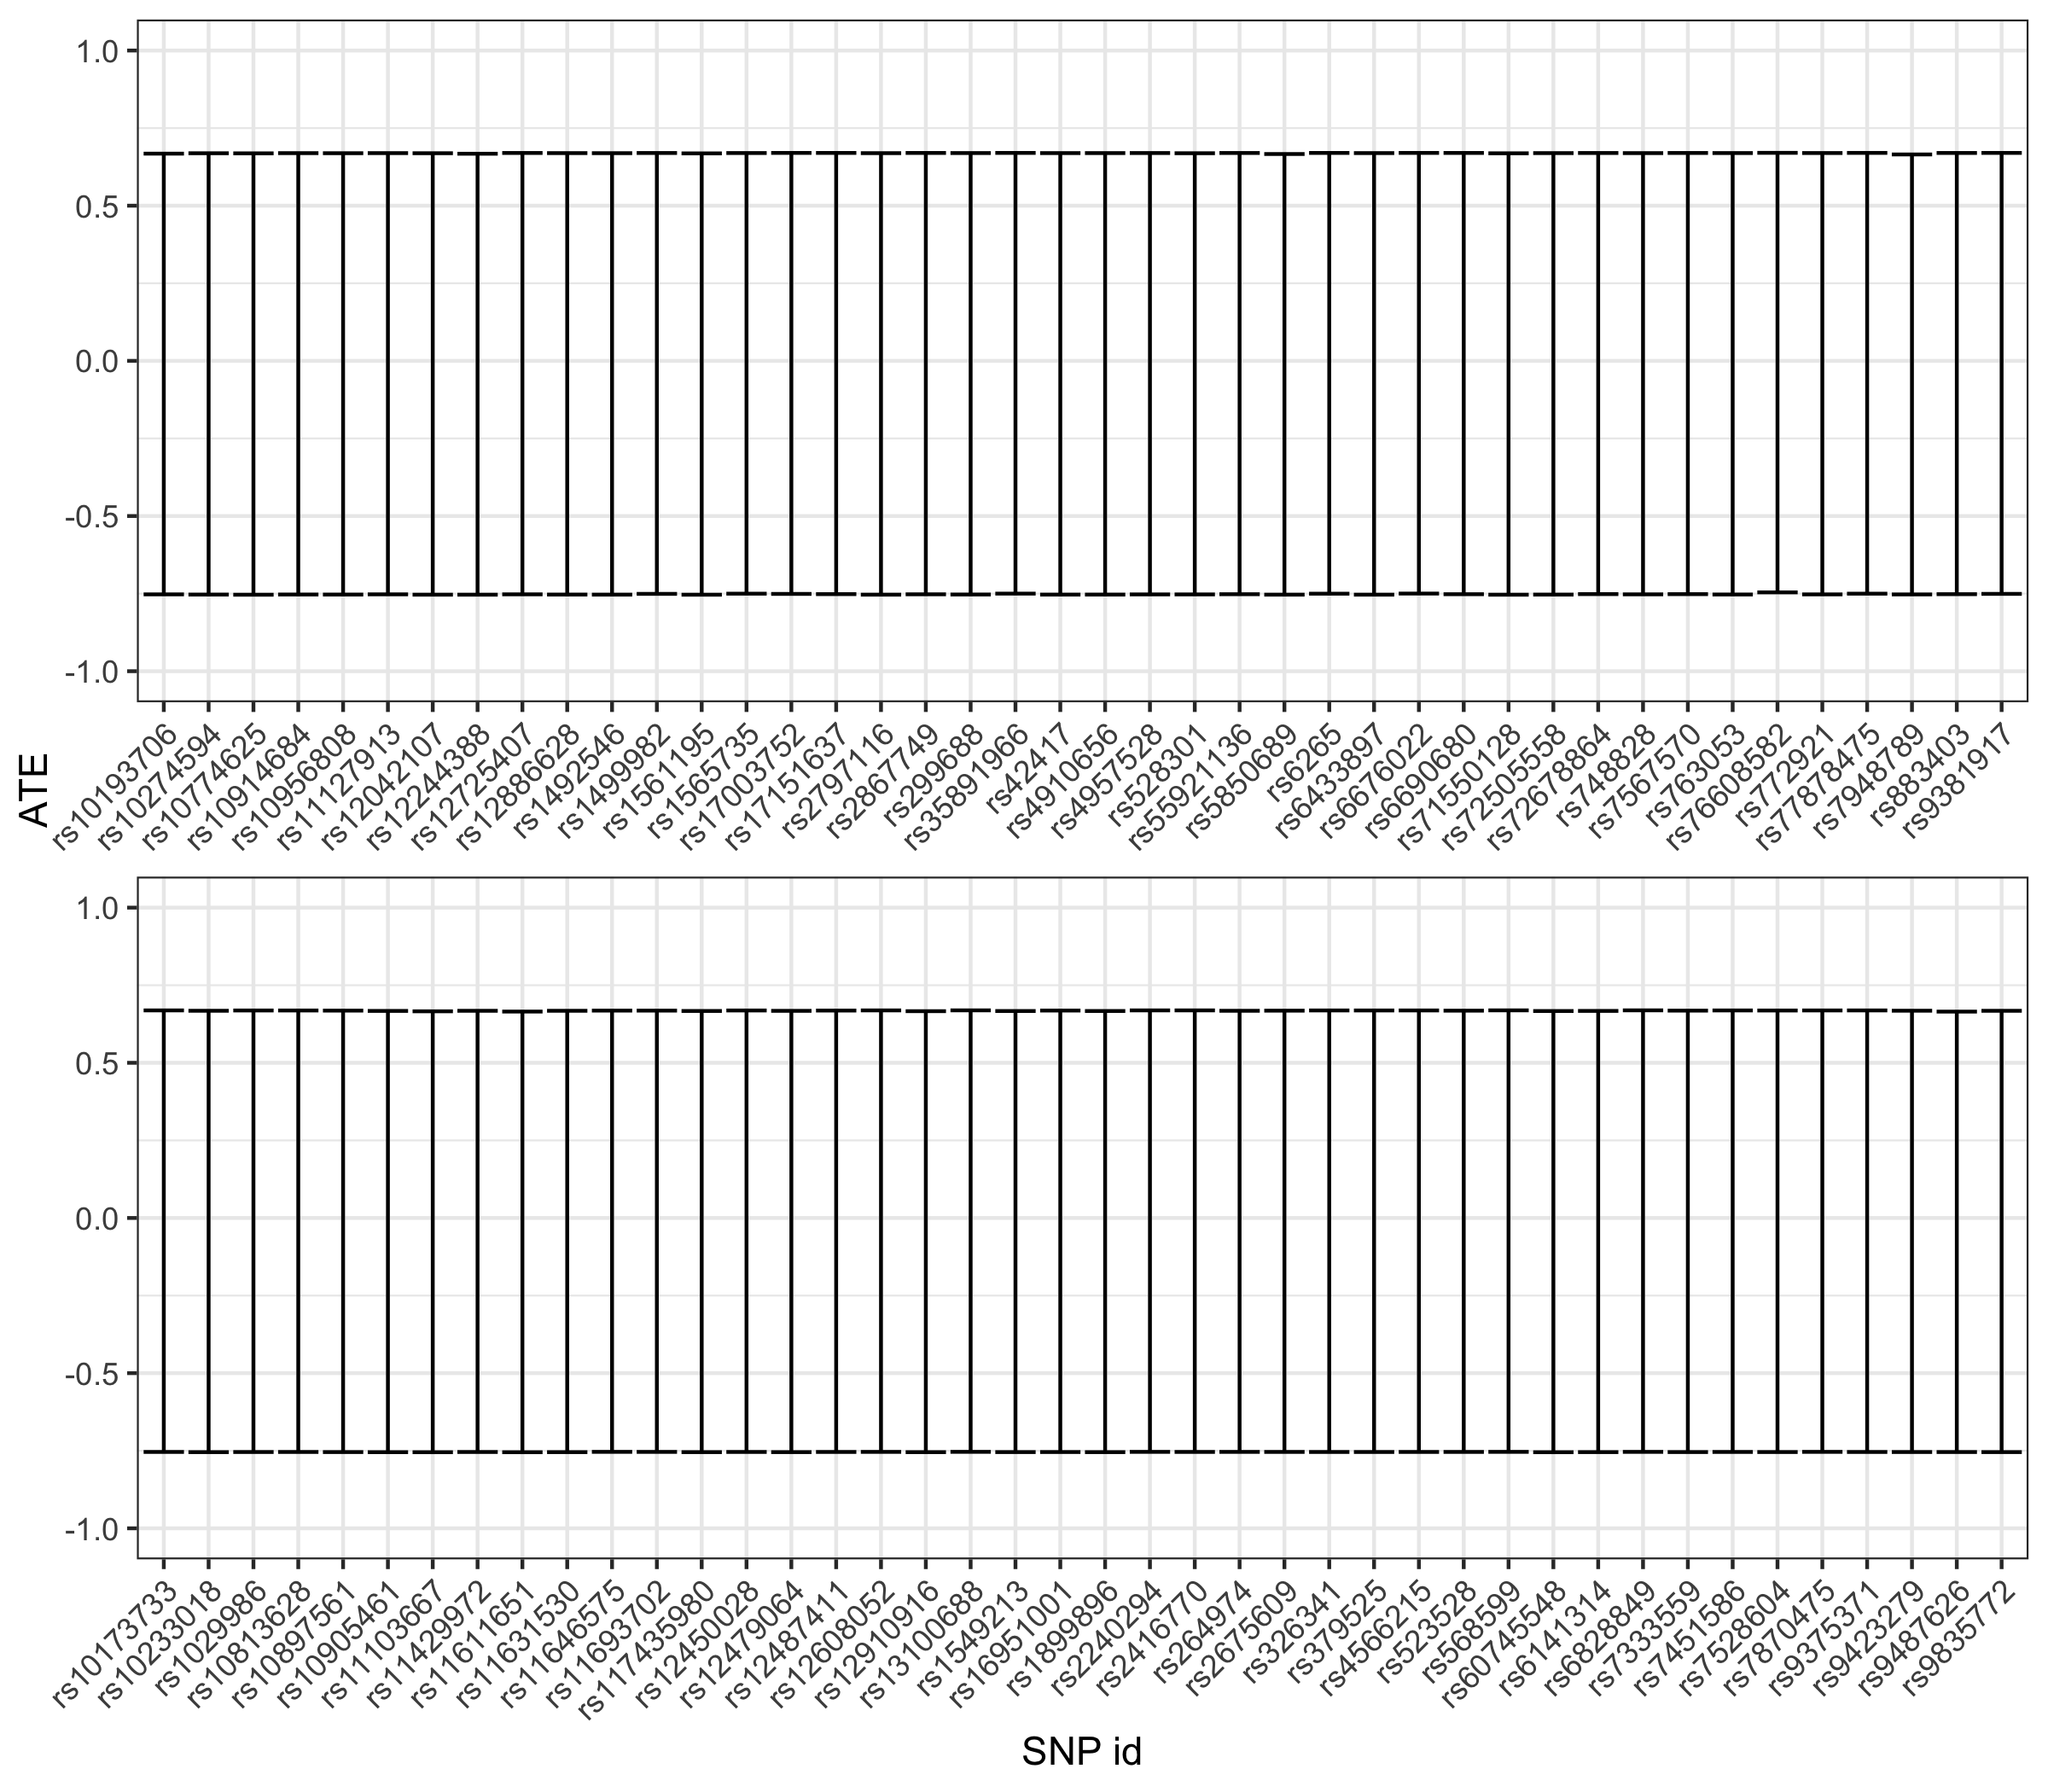
\includegraphics[width = 0.99\linewidth]{/Users/ralphtrane/Documents/RPackages_dev/ACEBounds/figures/example_analyses/smoking_depression_bivaraite_bounds_ukb-d-20116_0_ukb-d-20544_11.png}
  \caption{Non-parametric bounds for the 84 genetic variants identified as potential instruments for the effect of smoking on depression created based on the bivariate probabilities found from GWAS summary statistics.}
  \label{fig:smoking_on_depression_ind_bounds}
\end{figure}

With this in mind, we proceed to explore our quasi-bayesian approach. For each of the 84 genetic variants, we sample 500 potential trivariate distributions as described in Section \ref{quasi-bayesian}. From these 500 trivariate distributions, non-parametric bounds are created. Figure \ref{fig:smoking_on_depression_tri_bounds} shows the resulting bounds.

It is clear that while the trivariate bounds are much narrower than the corresponding bivariate bounds. This is very much so in line with our expectations. Unfortunately, all the bounds founds based on potential trivariate distributions overlap 0. This means that we will not be able to use non-parametric bounds to determine the direction of the ATE of smoking on the chances of developing depression, even if we were to obtain trivariate data.

\clearpage

\begin{sidewaysfigure}
  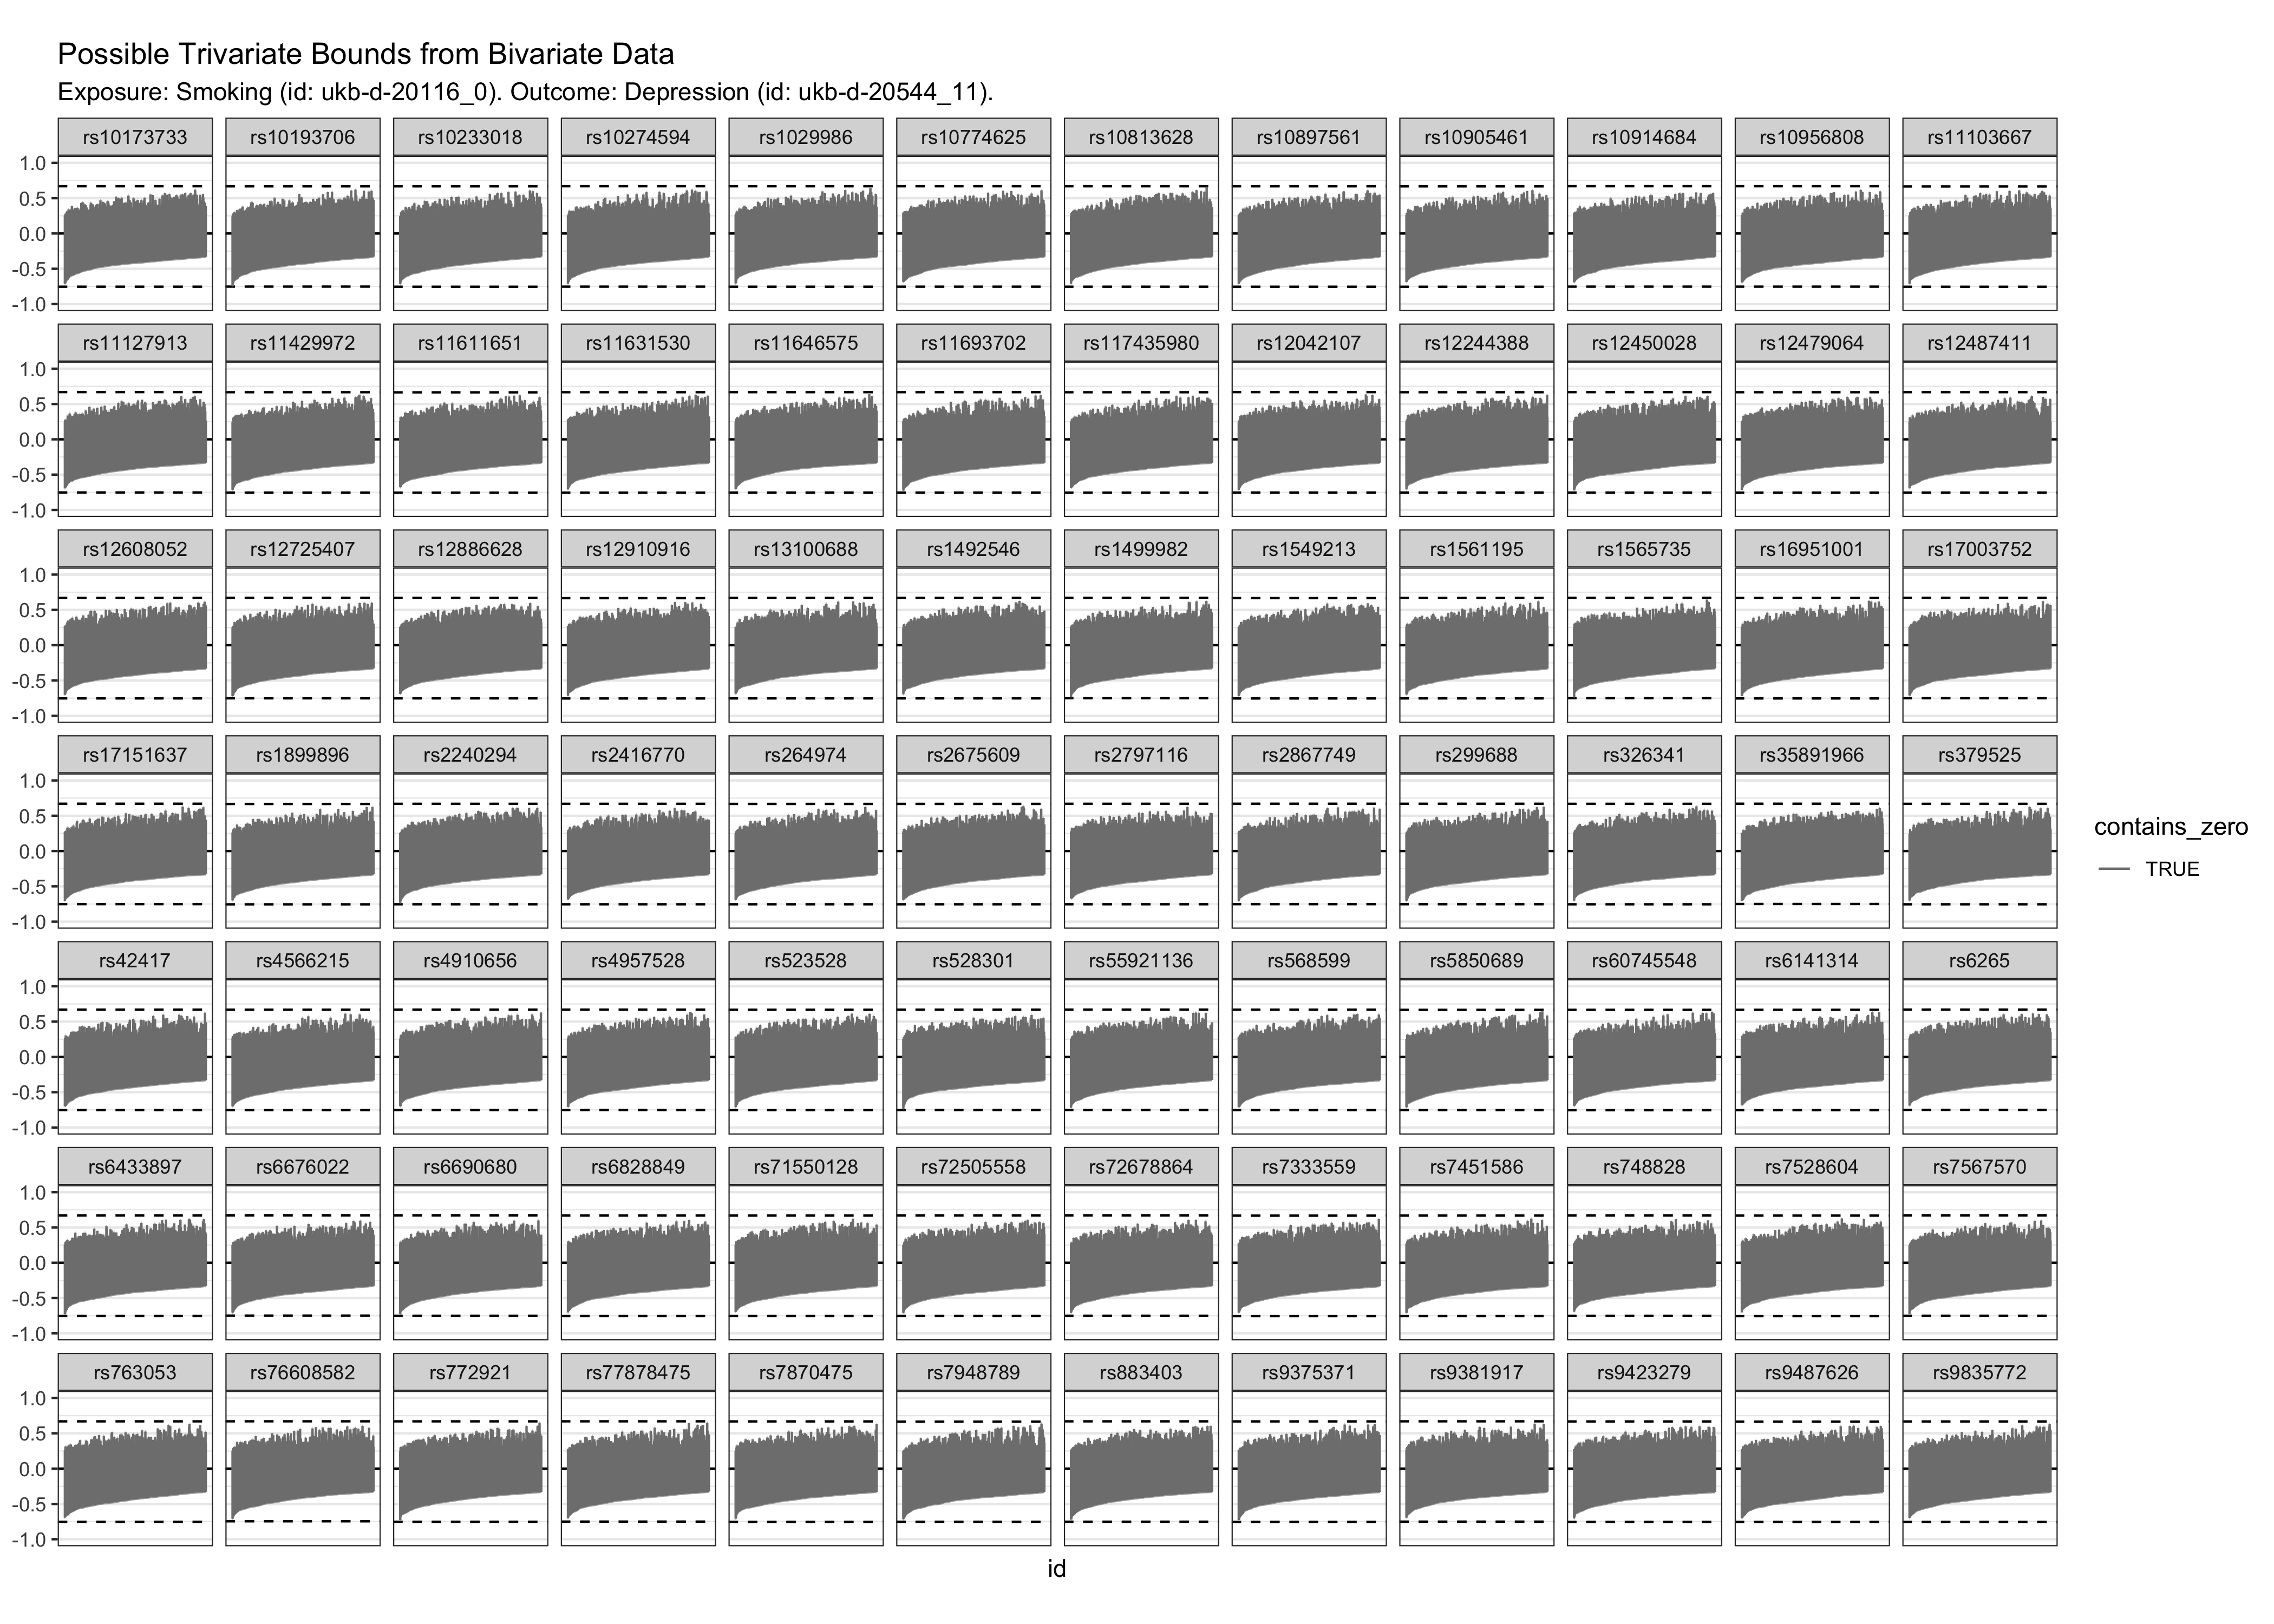
\includegraphics[width = 0.99\textheight]{/Users/ralphtrane/Documents/RPackages_dev/ACEBounds/figures/example_analyses/smoking_depression_individual_SNPs_plot_ukb-d-20116_0_ukb-d-20544_11.png}
    \caption{500 sets of bounds of the average treatment effect of smoking on depression for each of the 84 SNPs. Each bound is based on a set of values for the trivariate distribution randomly sampled. Bounds are color coded to show if they overlap 0 (grey) or do not (red). All bounds overlap 0.}
    \label{fig:smoking_on_depression_tri_bounds}
\end{sidewaysfigure}

\clearpage

Aggregating the information from multiple IVs through intersections is a simple idea, but everything we have seen so far points to this not being useful in practice. Figure \ref{fig:smoking_on_depression_intersections} shows the results from doing exactlt this for 9 pairs of SNPs, both when simply creating intersection of the bivariate bounds, and when using our quasi-bayesian approach to estimate the distribution of intersections of bounds from trivariate distributions as described in Section \ref{multiple-iv-case}. Comparing Figure \ref{fig:smoking_on_depression_intersections} to Figure \ref{fig:smoking_on_depression_tri_bounds}, we notice that the intersection bounds are essentially the same width. As for intersections of trivariate bounds, these are narrower than the corresponding intersections of bivariate bounds, but we do not see any scenario where intersections of trivariate bounds would help us determine direction of the ATE.

Again, the conclusion is that no sets of trivariate distributions allows us to determine direction of the average treatment effect through the use of non-parametric bounds.

\begin{figure}[H]
  \centering
  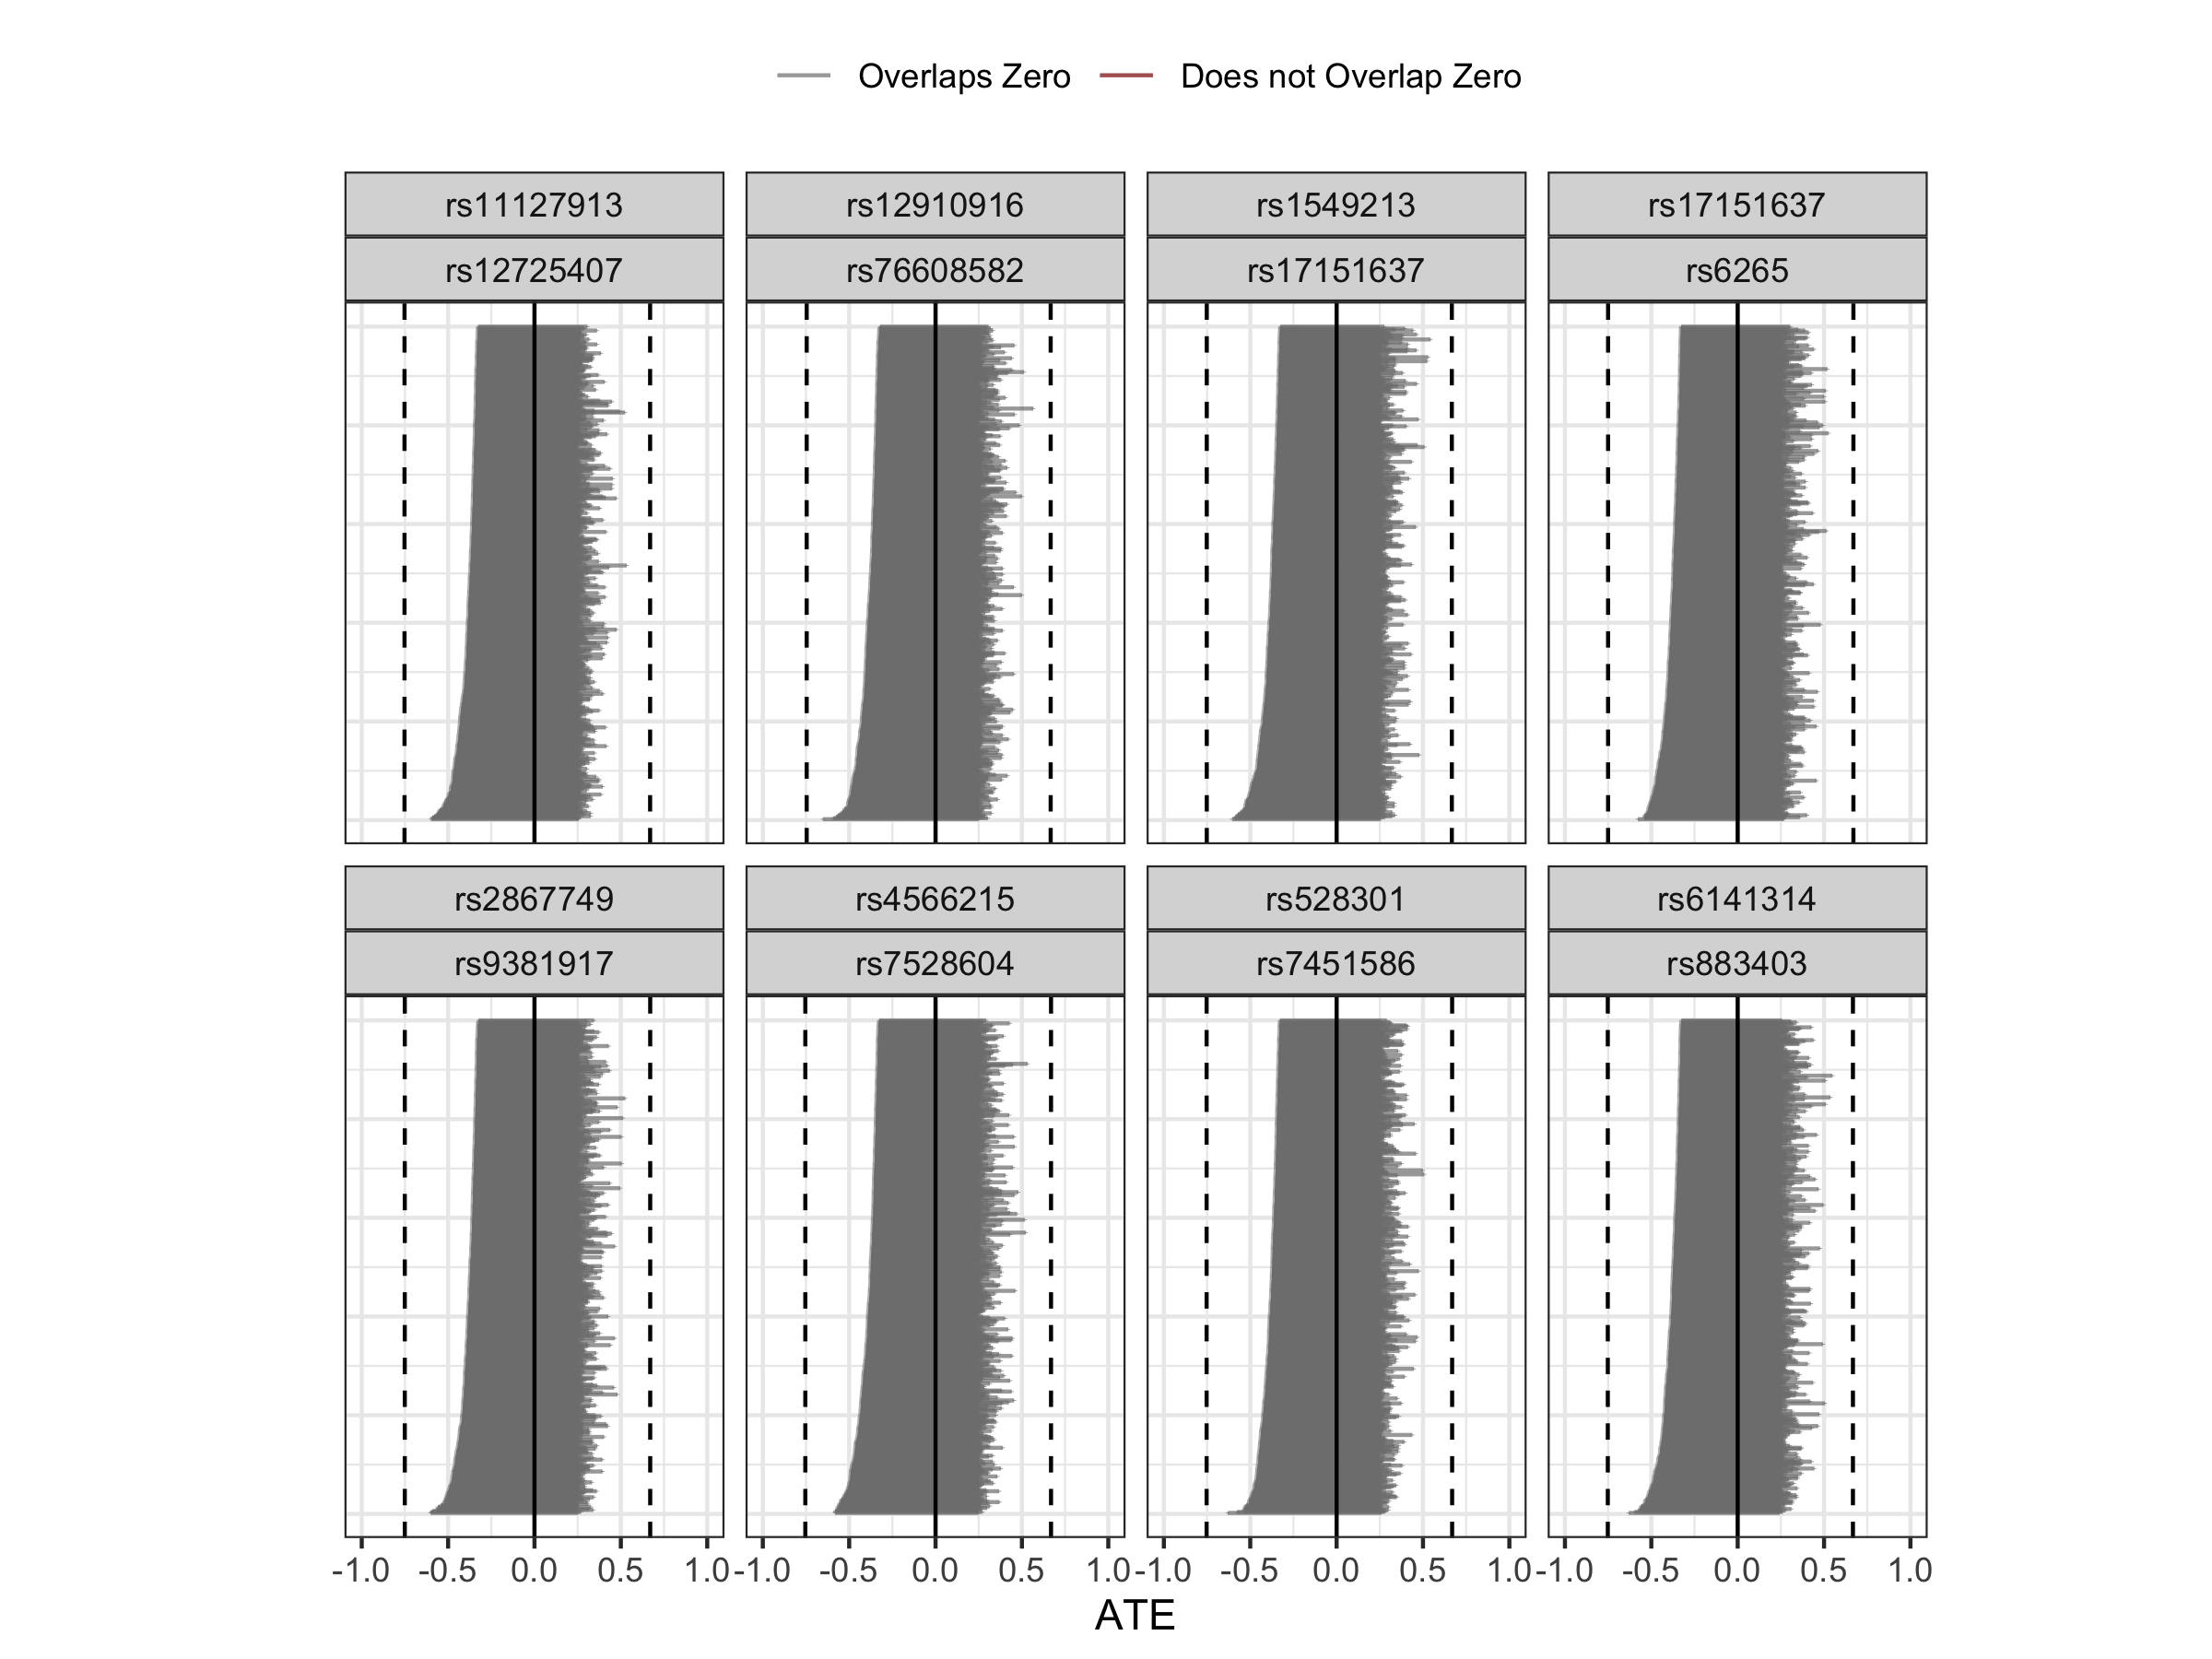
\includegraphics[width = 0.99\linewidth]{/Users/ralphtrane/Documents/RPackages_dev/ACEBounds/figures/example_analyses/smoking_depression_intersection_bounds_plot_ukb-d-20116_0_ukb-d-20544_11.png}
  \caption{Intersection bounds of the average treatment effect of smoking on depression based on randomly sampled trivariate distributions from pairs of SNPs. These 9 pairs were randomly chosen from all possible pairs.}
  \label{fig:smoking_on_depression_intersections}
\end{figure}

It is very important to keep in mind that this conclusion is only valid as long as the probabilities obtained are the true population probabilities. If this is the case, then non-parametric bounds simply will not allow us to determine direction of the ATE. The accuracy of the probabilities can be questioned, as these are derived from logistic regression results.

\hypertarget{smoking-effect-on-lung-cancer}{%
\subsection{Smoking effect on lung cancer}\label{smoking-effect-on-lung-cancer}}

As a positive control, we consider the effect of smoking on lung cancer. The general approach is a replicate of the previous section. Here, we obtain data on \((Y|Z)\) from the experiment in MRBase with id ukb-d-40001\_C349, while the data on \((X|Z)\) is again from the experiment with id ukb-d-20116\_0.

The SNPs used here are the same as in Section \ref{smoking-effect-on-depression}, and therefore the marginal conditional distributions and distribution of strengths are the same. More information on the instruments and summary statistics can be found in Appendix \ref{more-details-data-application-appendix}. Once again, the bivarate bounds (Figure \ref{fig:smoking_on_lung_cancer_ind_bounds}) are rather wide (all have width greater than 1) meaning they convey no truly useful information about the ATE, and even if we were to obtain trivariate data, we will not be able to determine the direction of the ATE (Figure \ref{fig:smoking_on_lung_cancer_tri_bounds}). Aggregating through intersections (Figure \ref{fig:smoking_on_lung_cancer_intersections}) does not lead to real gain in information, even if this is done using bounds based on trivariate distributions.

\begin{figure}[H]
  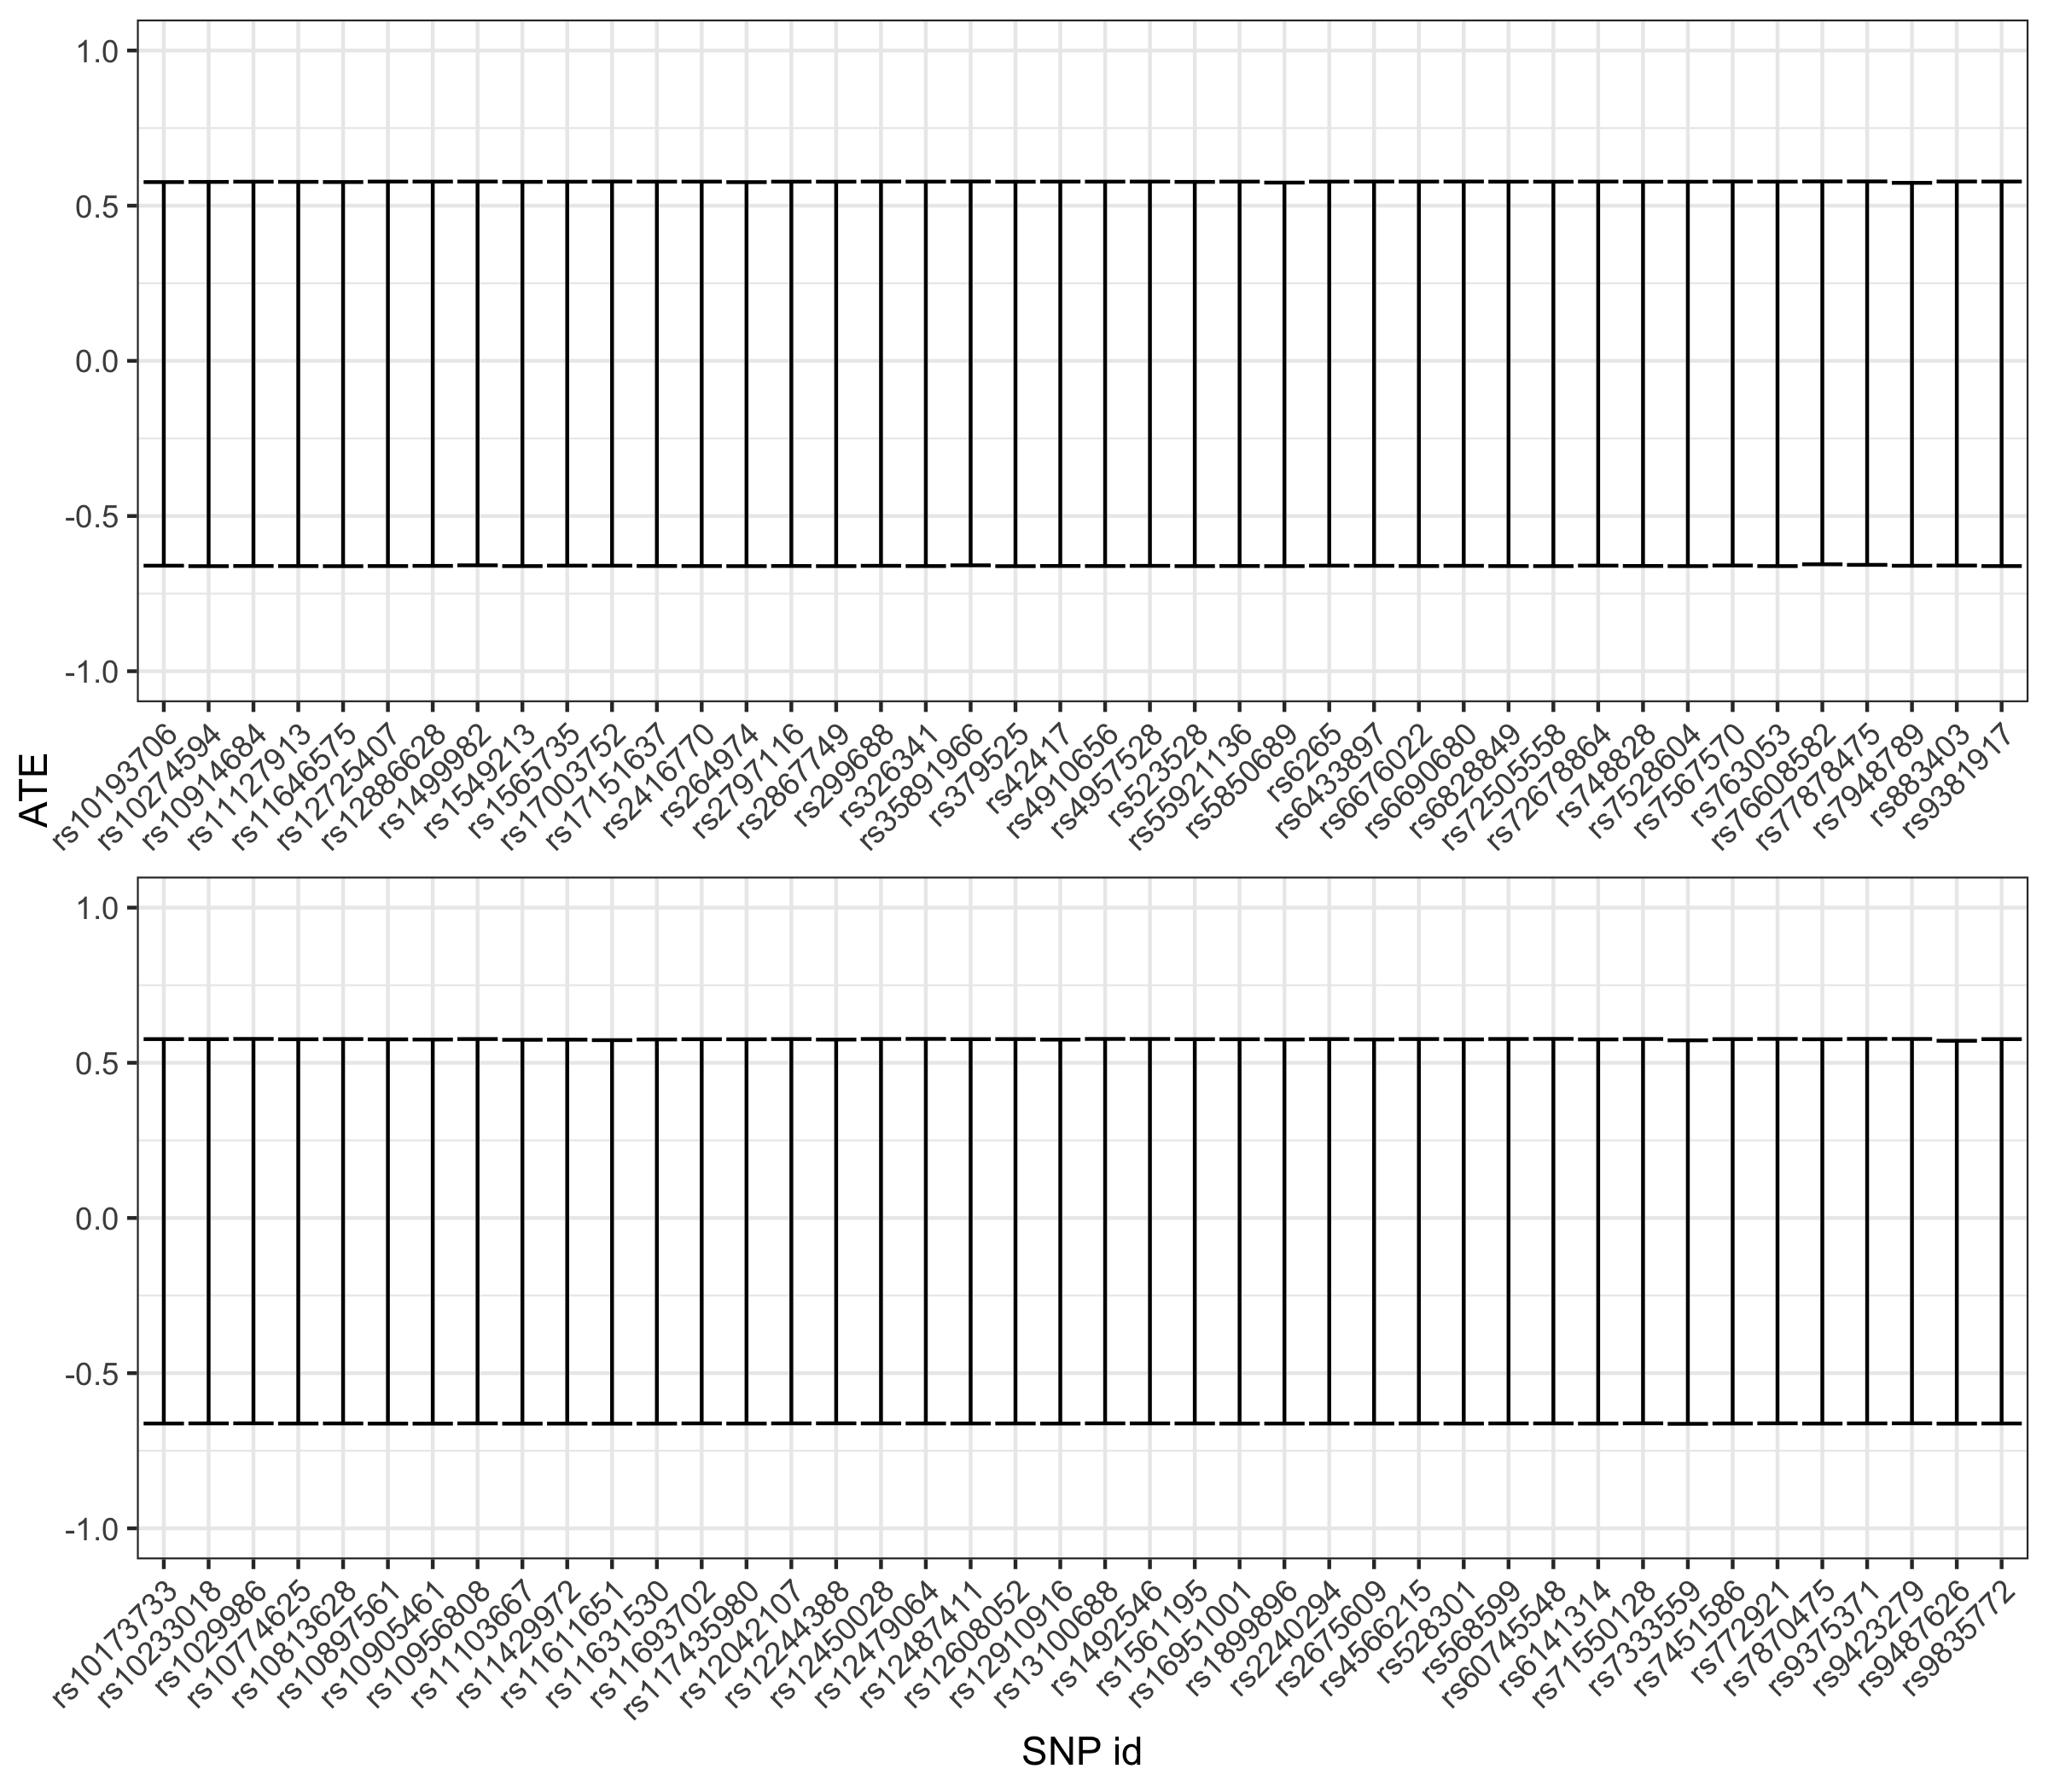
\includegraphics[width = 0.99\linewidth]{/Users/ralphtrane/Documents/RPackages_dev/ACEBounds/figures/example_analyses/smoking_lung_cancer_3_bivaraite_bounds_ukb-d-20116_0_ukb-d-40001_C349.png}
  \caption{Non-parametric bounds on the average treatment effect of smoking on lung cancer.}
  \label{fig:smoking_on_lung_cancer_ind_bounds}
\end{figure}

\clearpage

\begin{sidewaysfigure}
  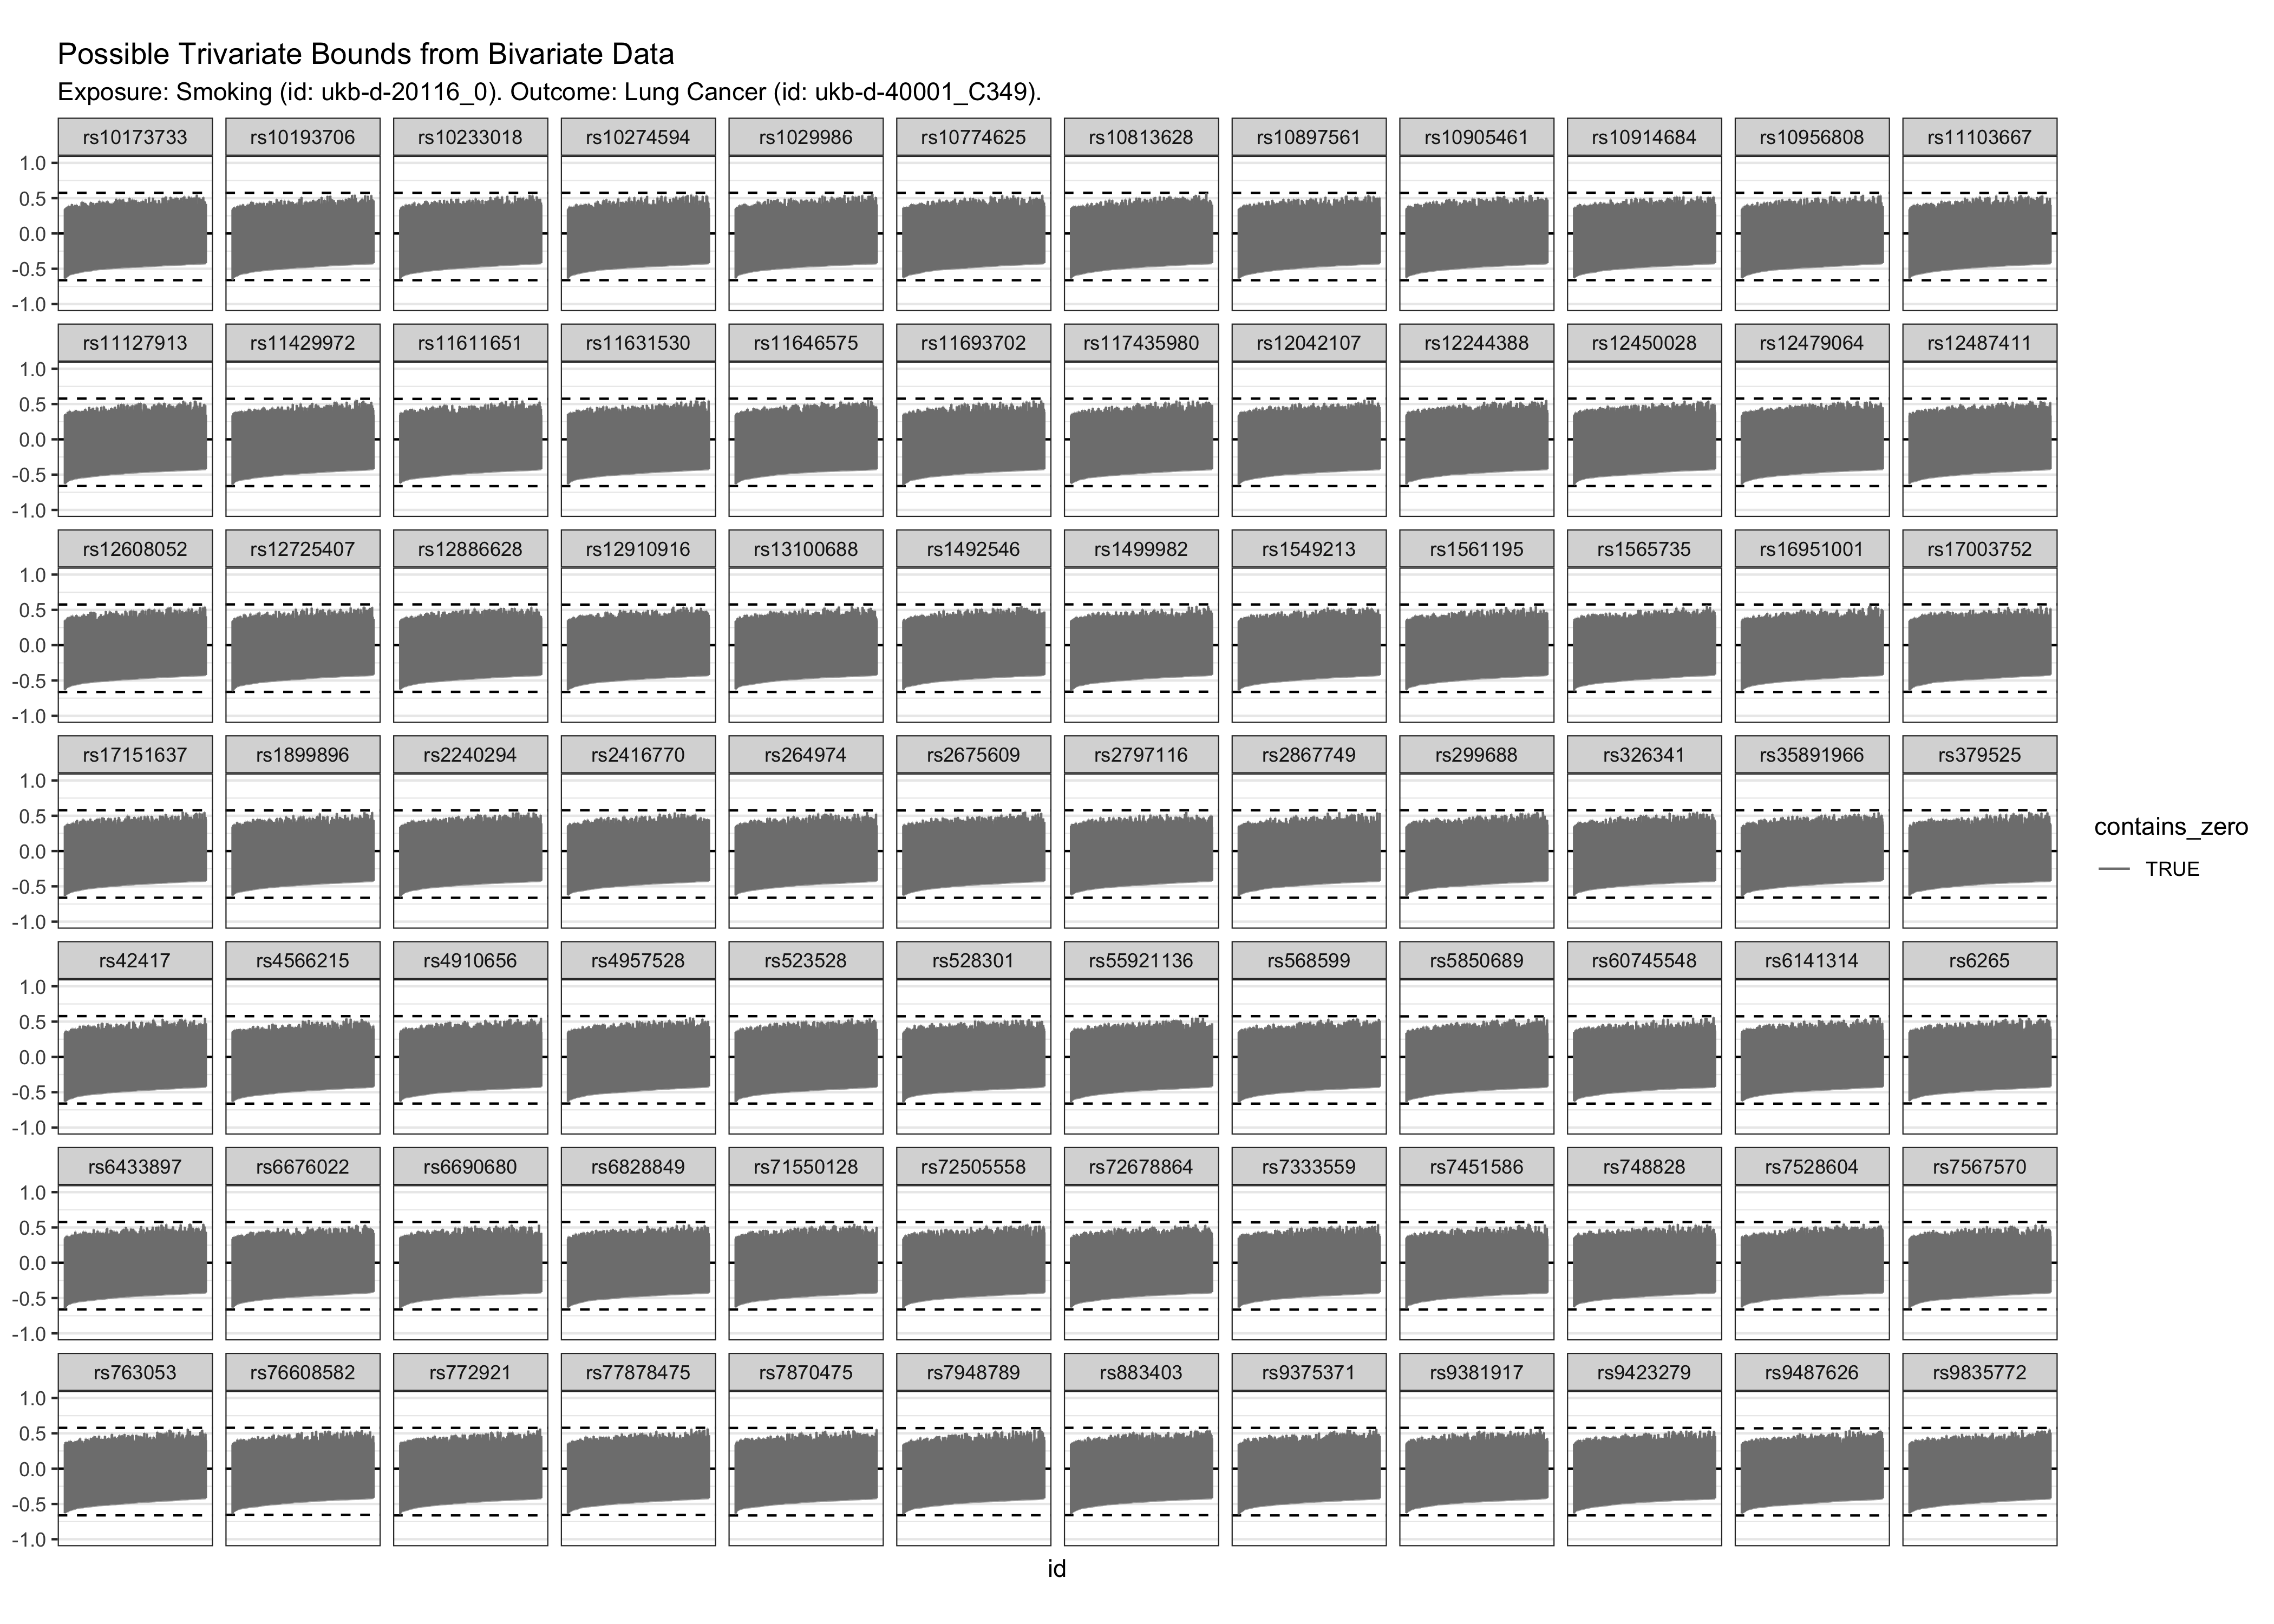
\includegraphics[width = 0.99\textheight]{/Users/ralphtrane/Documents/RPackages_dev/ACEBounds/figures/example_analyses/smoking_lung_cancer_3_individual_SNPs_plot_ukb-d-20116_0_ukb-d-40001_C349.png}
    \caption{500 sets of bounds of the average treatment effect of smoking on lung cancer for each of the 84 SNPs. Each bound is based on a set of values for the trivariate distribution randomyl sampled. Bounds are color coded to show if they overlap 0 (grey) or do not (red). All bounds overlap 0.}
    \label{fig:smoking_on_lung_cancer_tri_bounds}
\end{sidewaysfigure}

\clearpage

\begin{figure}[H]
  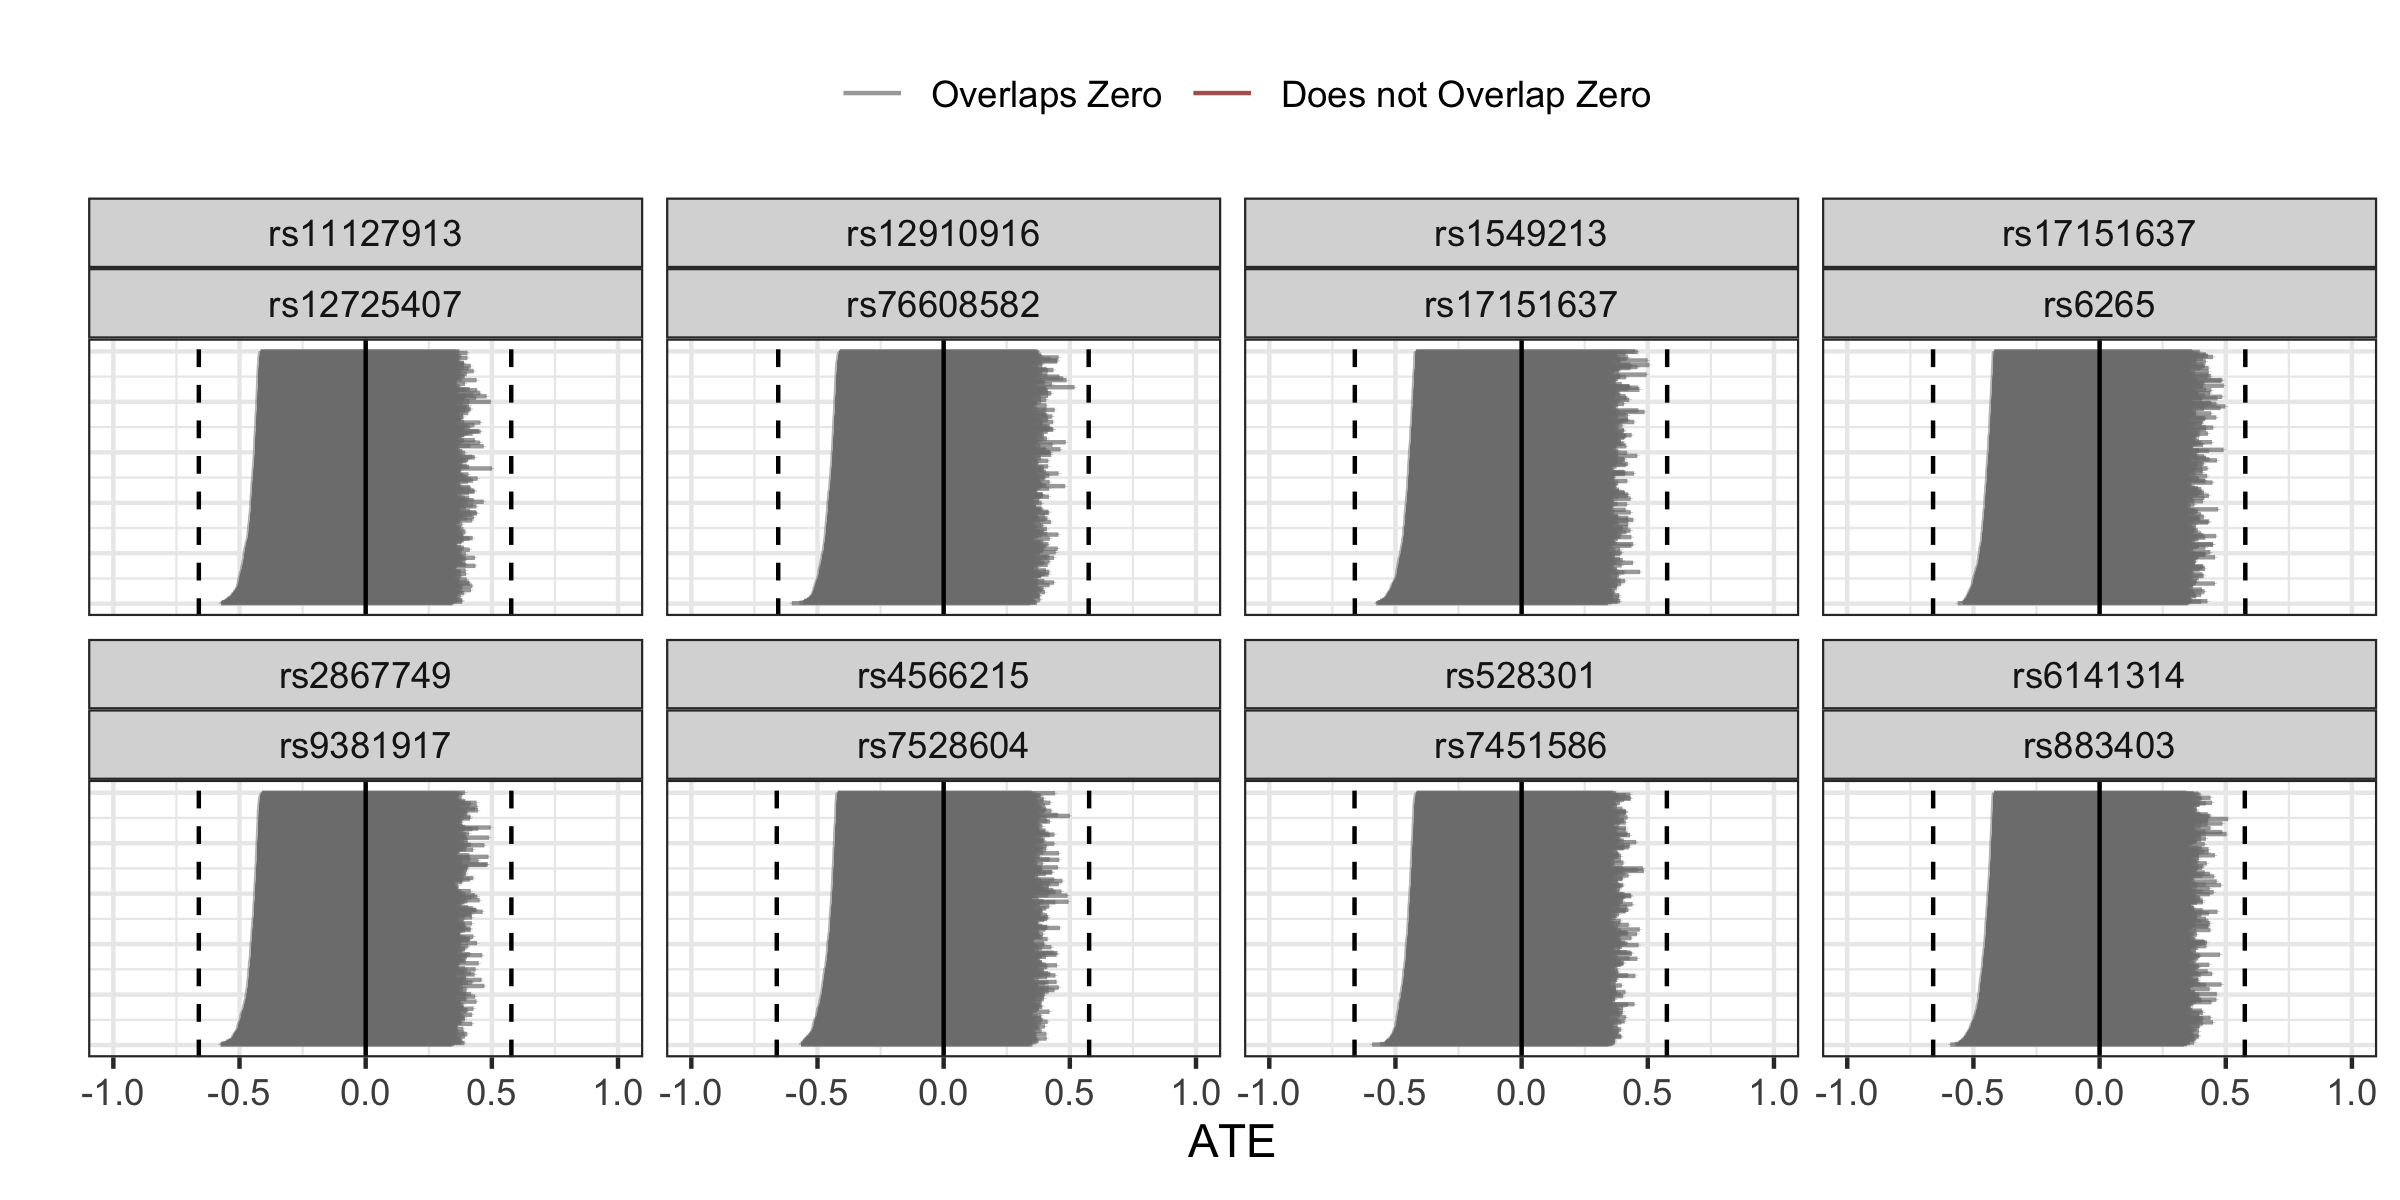
\includegraphics[width = 0.99\linewidth]{/Users/ralphtrane/Documents/RPackages_dev/ACEBounds/figures/example_analyses/smoking_lung_cancer_3_intersection_bounds_plot_ukb-d-20116_0_ukb-d-40001_C349.png}
  \caption{Intersection bounds of the average treatment effect of smoking on lung cancer based on randomly sampled trivariate distributions from pairs of SNPs. These 9 pairs were randomly chosen from all possible pairs.}
  \label{fig:smoking_on_lung_cancer_intersections}
\end{figure}

This is a very concerning result. It is well established that smoking has a strong causal effect on the chances of developing lung cancer (Cornfield et al. 1959). The fact that we are unable to say anything about the ATE in this case does not leave much hope in terms of future discoveries based on non-parametric bounds obtained using bivariate data. Even more concerning is the fact that trivariate distributions also are unsuccessful in determining the direction of the effect. Non-parametric bounds alone seem unable to give information about the direction of the effect, whether based on bivariate or trivariate data.

\newpage

\hypertarget{conclusion-and-practical-considerations}{%
\section{Conclusion and Practical Considerations}\label{conclusion-and-practical-considerations}}

Non-parametric bounds are without a doubt an attractive concept. With a minimal set of assumptions they let us obtain bounds on the average treatment effect in a deterministic way -- no probabilistic interpretations needed. It almost sounds to good to be true. As we have seen here, it turns out, in certain settings, it is.

While non-parametric bounds based on trivariate data come with very nice guarantees, such as the width always being less than 1, they are not applicable in Mendelian randomization analyses based on the kind of data that are made readily available through the many databases full of GWAS results. These databases contain information about bivariate data rather than trivariate data.

Fortunately, a framework for working out non-parametric bounds in this setting does exist (Ramsahai 2012), and it can be easily extended to many other scenarios, for example working with Instrumental Variables with more than two levels. Unfortunately, we lose the strong guarantees on the maximum width of the bounds we know from the trivariate bounds. To regain these guarantees, we need rather strong assumptions about the strength of the IV. Depending on the specific context, such strong IVs are very unlikely to be available.

Though information from bounds based on bivariate data might be limited, some is still available. Aggregating information from many instruments can be done in a simple fashion using intersections of individual bounds. This simple approach is only valid when all instruments are valid. In that case, it is a very reasonable way of aggregating information, but this will only result in significant gains of information when the individual bounds are shifted from one another, and not almost identical or nested. The problem with these non-parametric bounds is that the upper and lower bounds are close to monotonically decreasing and increasing, respectively, as a function of the strength. This means that intersections of bounds results in the set of bounds obtained from the strongest instrument, which leaves us with no more information than had we simply used the strongest instrument.

In a last effort to fully utilize the information we do have from bivariate data, we outline an approach to explore the potential trivariate distributions that are in agreement with the bivariate data at hand, and the bounds these potential trivariate distributions lead to. This gives us the opportunity to assess the conclusions non-parametric bounds from trivariate data could potentially lead to. One can use this to assess a posterior probability of the trivariate bounds containing zero, something that tells us if trivariate bounds are likely to be useful in determining direction of the average treatment effect, and could help guide a decision to further pursue an experiment aimed at collecting trivariate data. We considered a few different scenarios that provide different potential conclusions, and saw how diverse conclusions one can get to even when the original bivariate bounds are relatively similar. This suggests that we do indeed lose a lot of information in summarizing a trivariate distribution with only two bivariate distributions.

To demonstrate the use of non-parametric bounds in Mendelian randomization analyses, we considered two examples. In the first example, we aimed at finding bounds on the effect of smoking on the chances of developing depression. Unfortunately, all instruments available were very week with the strongest instrument having a strenght of less than \(0.01\). This results in bounds that provide very little information. Our quasi-bayesian approach suggests that even trivariate bounds would not be able to provide much extra information.

In our second example, we explored the effect of smoking on the chances of developing lung cancer. It has been well established that there is a rather strong causal effect of smoking on the chances of developing lung cancer. Unfortunately, our non-parametric bounds were not able to determine the direction of this effect, and our quasi-bayesian approach once again suggests that trivariate bounds would only bring a marginal improvement.

In this context, it is important to note that the conclusions made about the trivariate distributions only hold if the bivariate probabilities are correct. Whether that is the case here is questionable, as these probabilities are estimated based on logistic regression models.

Using genetic variants as instrumental variables is a very intriguing idea, but combining this setting with non-parametric bounds seems to give very few results. One potential use case of non-parametric bounds in a Mendelian randomization analysis could be when one has prior knowledge about the direction of the effect, but wish to get a better sense of the magnitude. Non-parametric bounds can provide an upper limit on this magnitude, which might in some scenarios be of use. For example in our second example, where the direction of the effect of smoking on lung cancer is well known, non-parametric bounds might help in providing an upper bound for the effect.

\newpage

\hypertarget{appendix-appendix}{%
\appendix}


\hypertarget{proof-of-theorem}{%
\section{\texorpdfstring{Proof of Theorem \ref{thm:upperBoundWidth}}{Proof of Theorem }}\label{proof-of-theorem}}

First of all, we note that the bounds found using the approach previously described when we impose both of the mentioned monotonicity assumptions are as follows:

\[
  \begin{aligned}
    &\max
      \begin{Bmatrix}
        -P(Y = 0 | Z = 2) - P(Y = 1 | Z = 0) + P(X = 0 | Z = 0) - P(X = 0 | Z = 2) \\
        P(Y = 0 | Z = 0) - 2\cdot P(Y = 0 | Z = 2) - P(X = 0 | Z = 2) \\
        -P(Y = 0 | Z = 2) - 2\cdot P(Y = 1 | Z = 0) + P(X = 0 | Z = 0)
      \end{Bmatrix} 
      \begin{matrix} (L1) \\ (L2) \\ (L3) \end{matrix}  \\
    &\qquad \qquad \qquad \qquad \qquad\le ATE \le \\
    &\min
      \begin{Bmatrix}
        1 + P(Y = 0 | Z = 0) - P(X = 0 | Z = 0) \\
        1 + P(Y = 0 | Z = 0) - P(Y = 0 | Z = 2) - P(X = 0 | Z = 0) + P(X = 0 | Z = 2) \\
        1 - P(Y = 0 | Z = 2) +  P(X = 0 | Z = 2)
      \end{Bmatrix}
      \begin{matrix} (U1) \\ (U2) \\ (U3) \end{matrix}
  \end{aligned}
\]

This gives us a total of nine different expressions for the width of the bounds. Since we assume monotonicity of the effect of \(Z\) on \(X\), the strength simplifies to \(\text{ST} = P(X = 1 | Z = 2) - P(X = 1 | Z = 0)\).

\textbf{Width = U1 - L1}

If the upper bound is \(U1\), \(U1 \le U2\), which implies \(P(Y = 0 | Z = 2) - P(X = 0 | Z = 2) \le 0\). Therefore,

\[\begin{aligned}
U1 - L1 &= 1 + P(Y = 0 | Z = 0) - P(X = 0 | Z = 0) + P(Y = 0 | Z = 2) + P(Y = 1 | Z = 0) - P(X = 0 | Z = 0) + P(X = 0 | Z = 2) \\
        &= 2 - ST + P(Y = 0 | Z = 2) - P(X = 0 | Z = 0) \\
        &= 2 - 2\cdot ST + P(Y = 0 | Z = 2) - P(X = 0 | Z = 2) \le 2 - 2\cdot ST.
\end{aligned}\]

\textbf{Width = U2 - L1}

\[\begin{aligned}
U2 - L1 &= 1 + P(Y = 0 | Z = 0) - P(Y = 0 | Z = 2) - P(X = 0 | Z = 0) + P(X = 0 | Z = 2) \\
        &\qquad + P(Y = 0 | Z = 2) + P(Y = 1 | Z = 0) - P(X = 0 | Z = 0) + P(X = 0 | Z = 2) \\
        &= 2 - 2\cdot ST
\end{aligned}\]

\textbf{Width = U3 - L1}

Since the upper bound is \(U3\), \(U3 \le U2\), which implies \(P(X = 0 | Z = 0) - P(Y = 0 | Z = 0) \le 0\). Therefore,

\[\begin{aligned}
U3 - L1 &= 1 - P(Y = 0 | Z = 2) +  P(X = 0 | Z = 2) + P(Y = 0 | Z = 2) + P(Y = 1 | Z = 0) - P(X = 0 | Z = 0) + P(X = 0 | Z = 2) \\
        &= 1 + P(Y = 1 | Z = 0) - ST + P(X = 0 | Z = 2) \\
        &= 2 - 2\cdot ST + P(X = 0 | Z = 0) - P(Y = 0 | Z = 0) \le 2 - 2 \cdot ST.
\end{aligned}\]

\textbf{Width = U1 - L2}

Since the upper bound is \(U1\), \(P(Y = 0 | Z = 2) \le P(X = 0 | Z = 2)\). Since the lower bound is \(L2\), \(L2 \ge L1\), which gives us \(1 - P(X = 0 | Z = 0) \ge P(Y = 0 | Z = 2)\). Therefore,

\[\begin{aligned}
U1 - L2 &= 1 + P(Y = 0 | Z = 0) - P(X = 0 | Z = 0) - P(Y = 0 | Z = 0) + 2\cdot P(Y = 0 | Z = 2) + P(X = 0 | Z = 2) \\
        &= 1 - ST + 2P(Y = 0 | Z = 2) \\
        &\le 2 - ST - P(X = 0 | Z = 0) + P(X = 0 | Z = 2) = 2 - 2\cdot ST.
\end{aligned}\]

\textbf{Width = U2 - L2}

Since the lower bound is \(L2\), \(1 - P(X = 0 | Z = 0) \ge P(Y = 0 | Z = 2)\). So,

\[\begin{aligned}
U2 - L2 &= 1 - P(X = 0 | Z = 0) + P(X = 0 | Z = 2) + P(Y = 0 | Z = 2) + P(X = 0 | Z = 2) \\
        &= 1 - ST + P(Y = 0 | Z = 2) + P(X = 0 | Z = 2) \\
        &\le 2 - 2\cdot ST.
\end{aligned}\]

\textbf{Width = U3 - L2}

Since the lower bound is \(L2\), \(1 - P(X = 0 | Z = 0) \ge P(Y = 0 | Z = 2)\). Since the upper bound is \(U3\), \(P(X = 0 | Z = 0) \le P(Y = 0 | Z = 0)\). Therefore,

\[\begin{aligned}
U3 - L2 &= 1 - P(Y = 0 | Z = 2) +  P(X = 0 | Z = 2) - P(Y = 0 | Z = 0) + 2\cdot P(Y = 0 | Z = 2) + P(X = 0 | Z = 2) \\
        &= 1 + 2\cdot P(X = 0 | Z = 2) + P(Y = 0 | Z = 2) - P(Y = 0 | Z = 0) \\
        &= 1 - 2\cdot ST + 2 P(X = 0 | Z = 0) + P(Y = 0 | Z = 2) - P(Y = 0 | Z = 0) \\
        &\le 2 - 2\cdot ST
\end{aligned}\]

\textbf{Width = U1 - L3}

Since the upper bound is \(U1\), \(P(Y = 0 | Z = 2) \le P(X = 0 | Z = 2)\). Since the lower bound is \(L3\), \(L3 \ge L1\), which implies \(P(Y = 1 | Z = 0) \le P(X = 0 | Z = 2)\). So,

\[\begin{aligned}
U1 - L3 &= 2 - P(X = 0 | Z = 0) + P(Y = 0 | Z = 2) + P(Y = 1 | Z = 0) - P(X = 0 | Z = 0) \\
        &= 2 - 2\cdot ST - 2\cdot P(X = 0 | Z = 2) + P(Y = 0 | Z = 2) + P(Y = 1 | Z = 0) \\
        &\le 2 - 2\cdot ST
\end{aligned}\]

\textbf{Width = U2 - L3}

Since the lower bound is \(L3\), \(P(Y = 1 | Z = 0) \le P(X = 0 | Z = 2)\)

\[\begin{aligned}
U2 - L3 &= 2 - 2\cdot P(X = 0 | Z = 0) + P(X = 0 | Z = 2) + P(Y = 1 | Z = 0) \\
        &= 2 - ST + P(Y = 1 | Z = 0) - P(X = 0 | Z = 0) \\
        &= 2 - 2\cdot ST + P(Y = 1 | Z = 0) - P(X = 0 | Z = 2) \le 2 - 2\cdot ST
\end{aligned}\]

\textbf{Width = U3 - L3}

Since the lower bound is \(L3\), \(P(Y = 1 | Z = 0) \le P(X = 0 | Z = 2)\). Since the upper bound is \(U3\), \(1 - P(X = 0 | Z = 0) \ge P(Y = 1 | Z = 0)\). Therefore,

\[\begin{aligned}
U3 - L3 &= 1 + P(X = 0 | Z = 2) + 2\cdot P(Y = 1 | Z = 0) - P(X = 0 | Z = 0) \\
        &\le 1 - ST + P(X = 0 | Z = 2) + 1 - P(X = 0 | Z = 0) \\
        &= 2 - 2\cdot ST.
\end{aligned}\]

\newpage

\hypertarget{exploration-of-scenarios-where-bounds-are-flipped}{%
\section{Exploration of Scenarios Where Bounds are Flipped}\label{exploration-of-scenarios-where-bounds-are-flipped}}

Of 10,000 randomly generated sets of values for \(P(X = 1 | Z = z), P(Y = 1 | Z = z),\ z = 0,1,2\), 123 resulted in bounds where the upper limit is smaller than the lower limit without violating any of the verifiable constraints presented in \eqref{eq:constraints}. Table \ref{tab:upper-less-than-lower} gives the values of the marginal conditional distributions with the strength of the IV, the corresponding bounds, and the width. It is notable that the IVs are rather strong in all cases where we see the bounds flip, but the bounds themselves and the widths vary quite a bit.

We first attributed this to the transition from trivariate to bivariate bounds, but later realized similar scenarios arise when dealing with trivariate bounds from four category IVs. Of 100,000 randomly generated sets of values for \(P(X = x, Y = y | Z = z),\ x=0,1,\ y=0,1,\ z=0,1,2,3\), 37 result in bounds where the upper limit is smaller than the lower limit without any violation of the verifiable constraints. It is also worth noting that in a similar number of trivariate distributions randomly generated with a trichotomous instrument, we did not see any cases of flipped bounds without a violation of one or more of the verifiable constraints. Table \ref{tab:flipped-trivariates} show the bounds from these trivariate distributions with the strengths of the IVs, and the width. Again, it is interesting to see the large span of widths and strengths present.

We have been unable to unearth a reason for why we see this phenomenon. One possible explanation is that the distributions that result in flipped bounds violate some uncheckable assumption.

\begingroup\fontsize{9}{11}\selectfont

\begin{landscape}
\begin{longtable}[t]{rrrrrrrrrr}
\caption{\label{tab:upper-less-than-lower}Marginal conditional probabilities resulting in bounds where the upper bound is smaller than the lower bound.}\\
\toprule
P(X=1|Z=0) & P(X=1|Z=1) & P(X=1|Z=2) & P(Y=1|Z=0) & P(Y=1|Z=1) & P(Y=1|Z=2) & Strength & Lower Bound & Upper Bound & Width\\
\midrule
\endfirsthead
\caption[]{\label{tab:upper-less-than-lower}Marginal conditional probabilities resulting in bounds where the upper bound is smaller than the lower bound. \textit{(continued)}}\\
\toprule
P(X=1|Z=0) & P(X=1|Z=1) & P(X=1|Z=2) & P(Y=1|Z=0) & P(Y=1|Z=1) & P(Y=1|Z=2) & Strength & Lower Bound & Upper Bound & Width\\
\midrule
\endhead

\endfoot
\bottomrule
\endlastfoot
0.2309955 & 0.3669268 & 0.9387298 & 0.8850137 & 0.3013143 & 0.9801302 & 0.7077343 & 0.5364056 & -0.0067221 & -0.5431277\\
0.9404491 & 0.4742722 & 0.1448868 & 0.0262469 & 0.5741507 & 0.1155472 & 0.7955623 & 0.0532826 & -0.4025552 & -0.4558377\\
0.8243777 & 0.0826950 & 0.6396267 & 0.0984834 & 0.0536095 & 0.6267494 & 0.7416826 & 0.3541403 & -0.0785379 & -0.4326782\\
0.6253430 & 0.7940521 & 0.0769966 & 0.7125237 & 0.1332569 & 0.0937761 & 0.7170556 & 0.3709784 & -0.0341142 & -0.4050925\\
0.4687418 & 0.9885571 & 0.0147455 & 0.4269904 & 0.0952051 & 0.1145516 & 0.9738116 & 0.1683963 & -0.2136943 & -0.3820906\\
\addlinespace
0.2384690 & 0.9589127 & 0.4551064 & 0.9411639 & 0.8220534 & 0.2995920 & 0.7204437 & 0.2623402 & -0.1057977 & -0.3681380\\
0.1201855 & 0.5087544 & 0.6903413 & 0.1553146 & 0.7813318 & 0.0153936 & 0.5701558 & 0.2303316 & -0.1312272 & -0.3615588\\
0.0558596 & 0.8249922 & 0.5150187 & 0.1693588 & 0.0317164 & 0.6019942 & 0.7691326 & 0.1515574 & -0.1885458 & -0.3401031\\
0.0601930 & 0.7105220 & 0.7764157 & 0.0349669 & 0.6138605 & 0.1288649 & 0.7162227 & 0.4235408 & 0.0910378 & -0.3325030\\
0.9689451 & 0.3369273 & 0.0921191 & 0.9728974 & 0.3379845 & 0.6435396 & 0.8768260 & 0.5457005 & 0.2351435 & -0.3105570\\
\addlinespace
0.0272617 & 0.9602504 & 0.7090107 & 0.9941238 & 0.7603751 & 0.5393045 & 0.9329888 & -0.0980534 & -0.3944198 & -0.2963664\\
0.8593575 & 0.5455747 & 0.0954651 & 0.7493743 & 0.2343858 & 0.8692962 & 0.7638924 & -0.0169223 & -0.3132765 & -0.2963542\\
0.0051370 & 0.7930864 & 0.6854693 & 0.0171757 & 0.5039197 & 0.0258429 & 0.7879494 & 0.4592943 & 0.1768274 & -0.2824669\\
0.8095621 & 0.0899196 & 0.7315497 & 0.1398438 & 0.0112235 & 0.5721541 & 0.7196425 & 0.3698677 & 0.0884094 & -0.2814583\\
0.0312864 & 0.5136612 & 0.7187288 & 0.1782691 & 0.7144743 & 0.0839332 & 0.6874423 & 0.2953632 & 0.0159345 & -0.2794287\\
\addlinespace
0.2841081 & 0.4642261 & 0.9303618 & 0.9272837 & 0.3015191 & 0.8563395 & 0.6462537 & 0.2718836 & 0.0151680 & -0.2567156\\
0.7020589 & 0.0426525 & 0.7537495 & 0.8146495 & 0.9551254 & 0.3030152 & 0.7110970 & -0.2695984 & -0.5219304 & -0.2523321\\
0.7299439 & 0.7079992 & 0.0126445 & 0.4179246 & 0.9411138 & 0.9059591 & 0.7172993 & -0.1196986 & -0.3687044 & -0.2490059\\
0.8553215 & 0.1611814 & 0.3987327 & 0.0868026 & 0.0650961 & 0.5766878 & 0.6941401 & 0.1241329 & -0.1137256 & -0.2378585\\
0.7503627 & 0.8262444 & 0.0255938 & 0.9023691 & 0.4826617 & 0.9697816 & 0.8006505 & -0.1771982 & -0.4057139 & -0.2285157\\
\addlinespace
0.7516532 & 0.1293625 & 0.6636683 & 0.2319998 & 0.0773707 & 0.8011377 & 0.6222907 & 0.3876713 & 0.1595554 & -0.2281159\\
0.1892072 & 0.6542341 & 0.6029697 & 0.9717090 & 0.8941221 & 0.2186525 & 0.4650268 & -0.1219402 & -0.3463509 & -0.2244107\\
0.9351863 & 0.1648035 & 0.3655840 & 0.1803887 & 0.1576169 & 0.6793117 & 0.7703828 & 0.0344709 & -0.1889068 & -0.2233777\\
0.8913881 & 0.2924893 & 0.1391987 & 0.0678851 & 0.5562612 & 0.1311623 & 0.7521894 & 0.0155394 & -0.2032671 & -0.2188065\\
0.2004629 & 0.8817321 & 0.4467427 & 0.2410824 & 0.0446975 & 0.7057212 & 0.6812692 & -0.1773694 & -0.3797903 & -0.2024209\\
\addlinespace
0.2713706 & 0.9177118 & 0.2155938 & 0.0584116 & 0.0235335 & 0.5341155 & 0.7021180 & -0.1254488 & -0.3224721 & -0.1970232\\
0.1716186 & 0.9793879 & 0.4387238 & 0.0758875 & 0.0913810 & 0.4572813 & 0.8077692 & -0.0377310 & -0.2332949 & -0.1955639\\
0.0346134 & 0.8601421 & 0.5243412 & 0.7170224 & 0.9940138 & 0.4402146 & 0.8255286 & 0.2680971 & 0.0753966 & -0.1927005\\
0.0517557 & 0.9490455 & 0.4763609 & 0.2257054 & 0.0428283 & 0.4666474 & 0.8972898 & -0.0882749 & -0.2790819 & -0.1908070\\
0.2097271 & 0.7849572 & 0.5591844 & 0.9851851 & 0.7694310 & 0.2353843 & 0.5752301 & -0.1266079 & -0.3155315 & -0.1889237\\
\addlinespace
0.8533233 & 0.5437889 & 0.3202183 & 0.0278734 & 0.0138157 & 0.8263378 & 0.5331050 & -0.2888714 & -0.4772378 & -0.1883664\\
0.0781475 & 0.4316186 & 0.9562902 & 0.6056942 & 0.2534086 & 0.8616394 & 0.8781427 & 0.3824505 & 0.1983152 & -0.1841354\\
0.7343532 & 0.7111032 & 0.0863323 & 0.4004145 & 0.9342732 & 0.9323079 & 0.6480209 & -0.1096618 & -0.2915366 & -0.1818748\\
0.4855778 & 0.2600183 & 0.9736867 & 0.3390356 & 0.9283873 & 0.7874292 & 0.7136685 & 0.1831962 & 0.0022975 & -0.1808987\\
0.6368154 & 0.0572293 & 0.8159708 & 0.5109590 & 0.0158577 & 0.1663634 & 0.7587416 & 0.3647850 & 0.1898262 & -0.1749588\\
\addlinespace
0.8824330 & 0.1367268 & 0.3081087 & 0.0653359 & 0.1951474 & 0.6000460 & 0.7457061 & -0.0637026 & -0.2342401 & -0.1705375\\
0.8090247 & 0.3226145 & 0.5675011 & 0.9402684 & 0.9741885 & 0.3180210 & 0.4864103 & 0.1805653 & 0.0148730 & -0.1656923\\
0.4510693 & 0.0872080 & 0.9033969 & 0.5323388 & 0.1710303 & 0.0969452 & 0.8161888 & 0.0158620 & -0.1452420 & -0.1611040\\
0.1518352 & 0.6975145 & 0.6509167 & 0.0629987 & 0.8097783 & 0.1657477 & 0.5456793 & 0.3801104 & 0.2198838 & -0.1602266\\
0.0653620 & 0.3813488 & 0.9612892 & 0.9275631 & 0.4953530 & 0.7515764 & 0.8959272 & -0.0696219 & -0.2290492 & -0.1594273\\
\addlinespace
0.2032074 & 0.7755576 & 0.4991361 & 0.7865987 & 0.9554554 & 0.2348516 & 0.5723502 & 0.2271745 & 0.0680689 & -0.1591056\\
0.0233274 & 0.6660489 & 0.8176706 & 0.8429973 & 0.2798561 & 0.7213751 & 0.7943432 & -0.2017648 & -0.3594838 & -0.1577189\\
0.9294752 & 0.2110150 & 0.4387583 & 0.1560685 & 0.0882931 & 0.6040925 & 0.7184602 & 0.0054762 & -0.1509059 & -0.1563822\\
0.1670113 & 0.6894123 & 0.4795673 & 0.0041910 & 0.8002859 & 0.0345400 & 0.5224010 & 0.4578813 & 0.3096595 & -0.1482218\\
0.3785346 & 0.9143229 & 0.1322393 & 0.3764540 & 0.9927913 & 0.6755701 & 0.7820836 & 0.4377743 & 0.2897923 & -0.1479819\\
\addlinespace
0.1776605 & 0.3763786 & 0.8762187 & 0.2525663 & 0.7852824 & 0.1601145 & 0.6985582 & -0.0751713 & -0.2174909 & -0.1423196\\
0.7676593 & 0.0086728 & 0.5238627 & 0.3109642 & 0.8841540 & 0.9821670 & 0.7589865 & -0.2989048 & -0.4399984 & -0.1410937\\
0.8834087 & 0.2154675 & 0.5237259 & 0.9402145 & 0.9094435 & 0.4479360 & 0.6679412 & 0.1993104 & 0.0599839 & -0.1393265\\
0.2128945 & 0.6634662 & 0.7020688 & 0.9859116 & 0.2297734 & 0.8227277 & 0.4891743 & -0.1801804 & -0.3162608 & -0.1360804\\
0.8197957 & 0.4539939 & 0.2933378 & 0.1292782 & 0.6944266 & 0.0241216 & 0.5264579 & 0.0595077 & -0.0754615 & -0.1349692\\
\addlinespace
0.8932091 & 0.2573860 & 0.3789772 & 0.8683447 & 0.8850420 & 0.3218777 & 0.6358231 & 0.2012298 & 0.0665657 & -0.1346641\\
0.3852521 & 0.7681010 & 0.1679198 & 0.6200211 & 0.0286245 & 0.1269667 & 0.6001813 & 0.0302481 & -0.0989742 & -0.1292223\\
0.4450183 & 0.3448027 & 0.9580487 & 0.0334938 & 0.6223715 & 0.0373602 & 0.6132460 & -0.3346527 & -0.4637484 & -0.1290957\\
0.9626206 & 0.3323393 & 0.3615993 & 0.8971357 & 0.8947940 & 0.3577061 & 0.6302814 & 0.3618066 & 0.2327966 & -0.1290100\\
0.9579589 & 0.2856719 & 0.2557011 & 0.0294142 & 0.0312341 & 0.4495460 & 0.7022578 & -0.1842660 & -0.3066353 & -0.1223693\\
\addlinespace
0.2722892 & 0.1030317 & 0.9532750 & 0.3335194 & 0.0179986 & 0.1046059 & 0.8502432 & 0.0914587 & -0.0308574 & -0.1223161\\
0.2075435 & 0.6267518 & 0.9907035 & 0.0610969 & 0.8711902 & 0.5325762 & 0.7831600 & 0.3339092 & 0.2125552 & -0.1213540\\
0.1309917 & 0.9511009 & 0.6110001 & 0.0092469 & 0.1382892 & 0.3862037 & 0.8201092 & 0.1057264 & -0.0118269 & -0.1175533\\
0.9469203 & 0.4771290 & 0.2975224 & 0.8483259 & 0.2756656 & 0.8366797 & 0.6493979 & 0.3148269 & 0.1973510 & -0.1174758\\
0.9141838 & 0.3947449 & 0.2582693 & 0.1776121 & 0.6284717 & 0.0485084 & 0.6559145 & 0.0149163 & -0.1016151 & -0.1165314\\
\addlinespace
0.2539480 & 0.3283935 & 0.9257231 & 0.5855638 & 0.1211694 & 0.0074839 & 0.6717752 & -0.3135619 & -0.4220422 & -0.1084803\\
0.7554315 & 0.0394385 & 0.8166883 & 0.9193390 & 0.1504442 & 0.4920783 & 0.7772497 & 0.5395735 & 0.4314412 & -0.1081323\\
0.5322302 & 0.8442719 & 0.1311744 & 0.7227207 & 0.1174348 & 0.2652317 & 0.7130975 & -0.0700917 & -0.1763950 & -0.1063033\\
0.1022484 & 0.7850567 & 0.3114329 & 0.9983873 & 0.9750404 & 0.6040354 & 0.6828082 & -0.0838413 & -0.1882423 & -0.1044009\\
0.8859779 & 0.1854690 & 0.2675919 & 0.9352886 & 0.8113619 & 0.3954484 & 0.7005089 & 0.2470847 & 0.1436625 & -0.1034222\\
\addlinespace
0.8858413 & 0.0577413 & 0.7457014 & 0.9231434 & 0.9814877 & 0.6837953 & 0.8281000 & -0.0658260 & -0.1636975 & -0.0978715\\
0.5688937 & 0.0533840 & 0.9092544 & 0.4161218 & 0.0847550 & 0.1385937 & 0.8558704 & 0.1398438 & 0.0425567 & -0.0972870\\
0.0111502 & 0.5785773 & 0.7360408 & 0.9491940 & 0.9715842 & 0.4417906 & 0.7248905 & -0.3414676 & -0.4342969 & -0.0928294\\
0.8016434 & 0.0919814 & 0.6269118 & 0.0598012 & 0.0080604 & 0.4024806 & 0.7096620 & 0.2023970 & 0.1138349 & -0.0885621\\
0.5613155 & 0.3343263 & 0.9641096 & 0.1739435 & 0.9413168 & 0.6466249 & 0.6297833 & 0.0475254 & -0.0400375 & -0.0875629\\
\addlinespace
0.9421035 & 0.7800406 & 0.0170238 & 0.6536674 & 0.8584000 & 0.0860958 & 0.9250797 & 0.6521608 & 0.5647278 & -0.0874330\\
0.4856718 & 0.1412137 & 0.8327200 & 0.2353279 & 0.7698770 & 0.8171080 & 0.6915064 & 0.0643282 & -0.0219988 & -0.0863269\\
0.7587967 & 0.2217142 & 0.4642144 & 0.1261614 & 0.0095185 & 0.6397095 & 0.5370825 & 0.1772441 & 0.0950201 & -0.0822241\\
0.8476325 & 0.0321449 & 0.5761561 & 0.7137147 & 0.9222930 & 0.4156565 & 0.8154876 & -0.2929622 & -0.3646398 & -0.0716776\\
0.8443266 & 0.0231323 & 0.6135112 & 0.5114541 & 0.9662261 & 0.9901356 & 0.8211943 & -0.3041605 & -0.3747334 & -0.0705729\\
\addlinespace
0.7090756 & 0.0306938 & 0.8591612 & 0.8275547 & 0.1987801 & 0.4221209 & 0.8284674 & 0.3686070 & 0.2983647 & -0.0702424\\
0.5210445 & 0.6877412 & 0.1936365 & 0.2077578 & 0.8583608 & 0.8895555 & 0.4941047 & -0.1155538 & -0.1840802 & -0.0685264\\
0.7325333 & 0.0360979 & 0.7452189 & 0.9243027 & 0.1841382 & 0.4150783 & 0.7091209 & 0.4838304 & 0.4154162 & -0.0684143\\
0.3112649 & 0.5408216 & 0.7700621 & 0.0719339 & 0.8911155 & 0.9844600 & 0.4587973 & 0.4371103 & 0.3713461 & -0.0657642\\
0.6839198 & 0.0601158 & 0.7429099 & 0.3546209 & 0.0832522 & 0.8458772 & 0.6827941 & 0.5591411 & 0.4955250 & -0.0636161\\
\addlinespace
0.4925476 & 0.1475428 & 0.6432137 & 0.1357593 & 0.7295215 & 0.9418075 & 0.4956709 & 0.0342830 & -0.0281982 & -0.0624812\\
0.0567614 & 0.4716677 & 0.8412115 & 0.9781020 & 0.6182925 & 0.8866750 & 0.7844501 & -0.1625195 & -0.2243887 & -0.0618691\\
0.1902110 & 0.3836209 & 0.9071890 & 0.8456573 & 0.3088491 & 0.0296753 & 0.7169780 & -0.5392827 & -0.6006846 & -0.0614020\\
0.3772296 & 0.8822068 & 0.2883994 & 0.2173902 & 0.9350335 & 0.7191264 & 0.5938073 & 0.4170904 & 0.3559363 & -0.0611541\\
0.5973862 & 0.8450983 & 0.2624347 & 0.1392309 & 0.6156584 & 0.9712264 & 0.5826636 & -0.2177176 & -0.2783525 & -0.0606348\\
\addlinespace
0.6339672 & 0.0297922 & 0.8123455 & 0.7376053 & 0.9506195 & 0.2630108 & 0.7825533 & -0.5198657 & -0.5786439 & -0.0587783\\
0.0823461 & 0.5840173 & 0.6679903 & 0.9677474 & 0.8284869 & 0.2712011 & 0.5856442 & -0.4461926 & -0.4996015 & -0.0534089\\
0.6535119 & 0.8883952 & 0.1073055 & 0.2820041 & 0.7154519 & 0.8117950 & 0.7810897 & -0.0743099 & -0.1269749 & -0.0526651\\
0.7404535 & 0.1312750 & 0.4474163 & 0.1314948 & 0.9068344 & 0.9347602 & 0.6091785 & -0.3671417 & -0.4196239 & -0.0524822\\
0.0820021 & 0.8994346 & 0.3178099 & 0.4734612 & 0.1446546 & 0.8253918 & 0.8174325 & -0.2855348 & -0.3349518 & -0.0494170\\
\addlinespace
0.0143154 & 0.1408971 & 0.9883829 & 0.5259441 & 0.4011591 & 0.9257180 & 0.9740675 & 0.4270428 & 0.3779018 & -0.0491410\\
0.5142074 & 0.8446779 & 0.0753746 & 0.5067568 & 0.0715657 & 0.1808748 & 0.7693032 & -0.0057421 & -0.0529810 & -0.0472389\\
0.1391137 & 0.4452852 & 0.7319911 & 0.0201224 & 0.4730480 & 0.0227584 & 0.5928773 & 0.1545757 & 0.1084867 & -0.0460890\\
0.7671998 & 0.0911903 & 0.9424491 & 0.7190755 & 0.0257481 & 0.5228183 & 0.8512587 & 0.4851985 & 0.4416630 & -0.0435356\\
0.2249334 & 0.9771968 & 0.6502243 & 0.9434316 & 0.7995282 & 0.4743734 & 0.7522634 & 0.0790767 & 0.0373769 & -0.0416998\\
\addlinespace
0.9124694 & 0.5503730 & 0.0400667 & 0.7951134 & 0.6099932 & 0.9632078 & 0.8724027 & -0.1948275 & -0.2362891 & -0.0414616\\
0.1645046 & 0.8060324 & 0.5635964 & 0.9246119 & 0.7605022 & 0.3061245 & 0.6415279 & -0.1730552 & -0.2140902 & -0.0410350\\
0.7079565 & 0.5723802 & 0.2806847 & 0.8839699 & 0.2430289 & 0.9515723 & 0.4272719 & -0.0591760 & -0.0987463 & -0.0395703\\
0.2097282 & 0.9124687 & 0.2747676 & 0.2570863 & 0.1285457 & 0.7024909 & 0.7027405 & -0.2311382 & -0.2703369 & -0.0391987\\
0.9736240 & 0.0208031 & 0.3737885 & 0.9045140 & 0.4334044 & 0.2716260 & 0.9528209 & 0.4846500 & 0.4464234 & -0.0382266\\
\addlinespace
0.1845828 & 0.1851770 & 0.8937890 & 0.8433725 & 0.4857333 & 0.9516657 & 0.7092062 & 0.2051761 & 0.1681541 & -0.0370221\\
0.1904095 & 0.9898458 & 0.0778574 & 0.3241436 & 0.0396418 & 0.5826816 & 0.9119883 & -0.4464247 & -0.4830894 & -0.0366648\\
0.3058563 & 0.8758829 & 0.3221585 & 0.8338573 & 0.0715108 & 0.2981029 & 0.5700266 & -0.4066656 & -0.4426015 & -0.0359359\\
0.5517228 & 0.8850872 & 0.1379439 & 0.7797196 & 0.3208303 & 0.1888349 & 0.7471432 & 0.1261619 & 0.0917667 & -0.0343952\\
0.0614376 & 0.2965834 & 0.9979328 & 0.0027831 & 0.1401460 & 0.0597136 & 0.9364952 & 0.0117046 & -0.0165844 & -0.0282890\\
\addlinespace
0.8779495 & 0.4096741 & 0.2304406 & 0.7998226 & 0.4274697 & 0.9938156 & 0.6475089 & -0.0719255 & -0.0992804 & -0.0273549\\
0.6979215 & 0.7737010 & 0.0234315 & 0.9852010 & 0.4651610 & 0.8182570 & 0.7502694 & -0.0989160 & -0.1244899 & -0.0255739\\
0.6623782 & 0.7107869 & 0.1608789 & 0.9024376 & 0.2805005 & 0.8890312 & 0.5499081 & -0.1508689 & -0.1758042 & -0.0249354\\
0.4107040 & 0.6300393 & 0.0755462 & 0.7135503 & 0.0247311 & 0.2318819 & 0.5544931 & 0.0986941 & 0.0758333 & -0.0228608\\
0.2389620 & 0.9996788 & 0.3607017 & 0.1224239 & 0.2775328 & 0.6499732 & 0.7607167 & -0.0727986 & -0.0942652 & -0.0214665\\
\addlinespace
0.2466505 & 0.3150522 & 0.9973913 & 0.7941729 & 0.4943148 & 0.9589104 & 0.7507408 & 0.4182885 & 0.3992699 & -0.0190186\\
0.1047963 & 0.5872602 & 0.6265764 & 0.1702907 & 0.0689137 & 0.7661262 & 0.5217801 & 0.2159521 & 0.1971807 & -0.0187714\\
0.6454304 & 0.5477765 & 0.0021959 & 0.8270074 & 0.1628806 & 0.2007895 & 0.6432345 & 0.4210367 & 0.4032008 & -0.0178359\\
0.0147348 & 0.9403617 & 0.7719393 & 0.1339251 & 0.5201033 & 0.7372833 & 0.9256270 & 0.4399636 & 0.4221999 & -0.0177637\\
0.6149141 & 0.1287129 & 0.8052456 & 0.3774013 & 0.9281094 & 0.7809966 & 0.6765327 & -0.2049168 & -0.2213916 & -0.0164747\\
\addlinespace
0.6318831 & 0.8417779 & 0.1046526 & 0.1803197 & 0.6822984 & 0.0227946 & 0.7371254 & 0.4274041 & 0.4145748 & -0.0128292\\
0.4658334 & 0.1177519 & 0.8202813 & 0.3008471 & 0.8740505 & 0.7295855 & 0.7025294 & -0.2011135 & -0.2117500 & -0.0106365\\
0.4692894 & 0.9793264 & 0.2505315 & 0.6858286 & 0.3586177 & 0.0507586 & 0.7287948 & 0.0832484 & 0.0727541 & -0.0104943\\
0.9053262 & 0.4920161 & 0.2908324 & 0.8237065 & 0.8801458 & 0.1128271 & 0.6144939 & 0.3452384 & 0.3365678 & -0.0086706\\
0.8400507 & 0.6066834 & 0.0207922 & 0.8392446 & 0.3014262 & 0.1199182 & 0.8192585 & 0.5578239 & 0.5502410 & -0.0075829\\
\addlinespace
0.2986999 & 0.3574011 & 0.7508847 & 0.7003727 & 0.1246649 & 0.9739429 & 0.4521849 & 0.3249903 & 0.3213192 & -0.0036711\\
0.0463115 & 0.4417234 & 0.7452841 & 0.1110238 & 0.4748895 & 0.0612693 & 0.6989726 & 0.1602189 & 0.1570808 & -0.0031381\\
0.8543023 & 0.0104242 & 0.1896705 & 0.9925313 & 0.2311163 & 0.0674310 & 0.8438782 & 0.6262363 & 0.6260467 & -0.0001896\\*
\end{longtable}
\end{landscape}
\endgroup{}

\begin{longtable}[t]{rrrr}
\caption{\label{tab:flipped-trivariates}Lower and Upper limits of bounds where the upper limit is less than the lower limit for trivariate distributions with four category instruments.}\\
\toprule
Lower & Upper & Strength & Width\\
\midrule
\endfirsthead
\caption[]{\label{tab:flipped-trivariates}Lower and Upper limits of bounds where the upper limit is less than the lower limit for trivariate distributions with four category instruments. \textit{(continued)}}\\
\toprule
Lower & Upper & Strength & Width\\
\midrule
\endhead

\endfoot
\bottomrule
\endlastfoot
0.1796920 & 0.0395535 & 0.0853119 & -0.1401385\\
-0.0038326 & -0.1264492 & 0.1539099 & -0.1226166\\
-0.0169573 & -0.1304422 & 0.2235469 & -0.1134849\\
-0.0620851 & -0.1743916 & 0.0805434 & -0.1123066\\
0.0996764 & -0.0065497 & 0.2112420 & -0.1062260\\
\addlinespace
-0.0348047 & -0.1393748 & 0.1884223 & -0.1045701\\
-0.0097177 & -0.1102060 & 0.0874967 & -0.1004882\\
-0.0470850 & -0.1435686 & 0.1458296 & -0.0964835\\
-0.1052398 & -0.1993785 & 0.2667633 & -0.0941387\\
0.1097975 & 0.0268471 & 0.1774704 & -0.0829504\\
\addlinespace
0.1884781 & 0.1110487 & 0.3297432 & -0.0774293\\
0.0174359 & -0.0580424 & 0.2058740 & -0.0754784\\
-0.0530855 & -0.1187770 & 0.2521754 & -0.0656915\\
0.0534080 & -0.0107149 & 0.1509847 & -0.0641230\\
-0.0660707 & -0.1258819 & 0.2831483 & -0.0598112\\
\addlinespace
0.3495840 & 0.2945716 & 0.3633999 & -0.0550124\\
0.1665198 & 0.1136389 & 0.2131245 & -0.0528809\\
-0.0356540 & -0.0879713 & 0.2476628 & -0.0523173\\
0.1089847 & 0.0575836 & 0.1941017 & -0.0514012\\
0.0086756 & -0.0338341 & 0.2340061 & -0.0425097\\
\addlinespace
0.1335166 & 0.0930974 & 0.4555966 & -0.0404192\\
0.1163970 & 0.0761754 & 0.1573917 & -0.0402216\\
-0.1249197 & -0.1611461 & 0.1712798 & -0.0362264\\
-0.1252239 & -0.1581375 & 0.1035529 & -0.0329136\\
-0.2954311 & -0.3273509 & 0.3077593 & -0.0319199\\
\addlinespace
0.0274287 & -0.0007244 & 0.0813449 & -0.0281530\\
-0.1317444 & -0.1586467 & 0.3469784 & -0.0269023\\
0.1050533 & 0.0818064 & 0.2388595 & -0.0232469\\
-0.1980031 & -0.2156885 & 0.2205149 & -0.0176854\\
0.0408272 & 0.0265662 & 0.1314643 & -0.0142609\\
\addlinespace
0.1255375 & 0.1131666 & 0.0426523 & -0.0123709\\
-0.1421790 & -0.1523644 & 0.1409053 & -0.0101854\\
-0.0997312 & -0.1083943 & 0.3816466 & -0.0086630\\
-0.0304169 & -0.0353880 & 0.1323408 & -0.0049711\\
0.0094786 & 0.0046709 & 0.2838685 & -0.0048077\\
\addlinespace
-0.0217285 & -0.0245811 & 0.3531008 & -0.0028526\\
-0.0563955 & -0.0583218 & 0.4092683 & -0.0019263\\*
\end{longtable}

\hypertarget{additional-summary-statistics-for-analyses-presented-in-section}{%
\section{\texorpdfstring{Additional Summary Statistics for Analyses Presented in Section \ref{data-analysis} \label{more-details-data-application-appendix}}{Additional Summary Statistics for Analyses Presented in Section  }}\label{additional-summary-statistics-for-analyses-presented-in-section}}

\begin{figure}[H]
  \center
  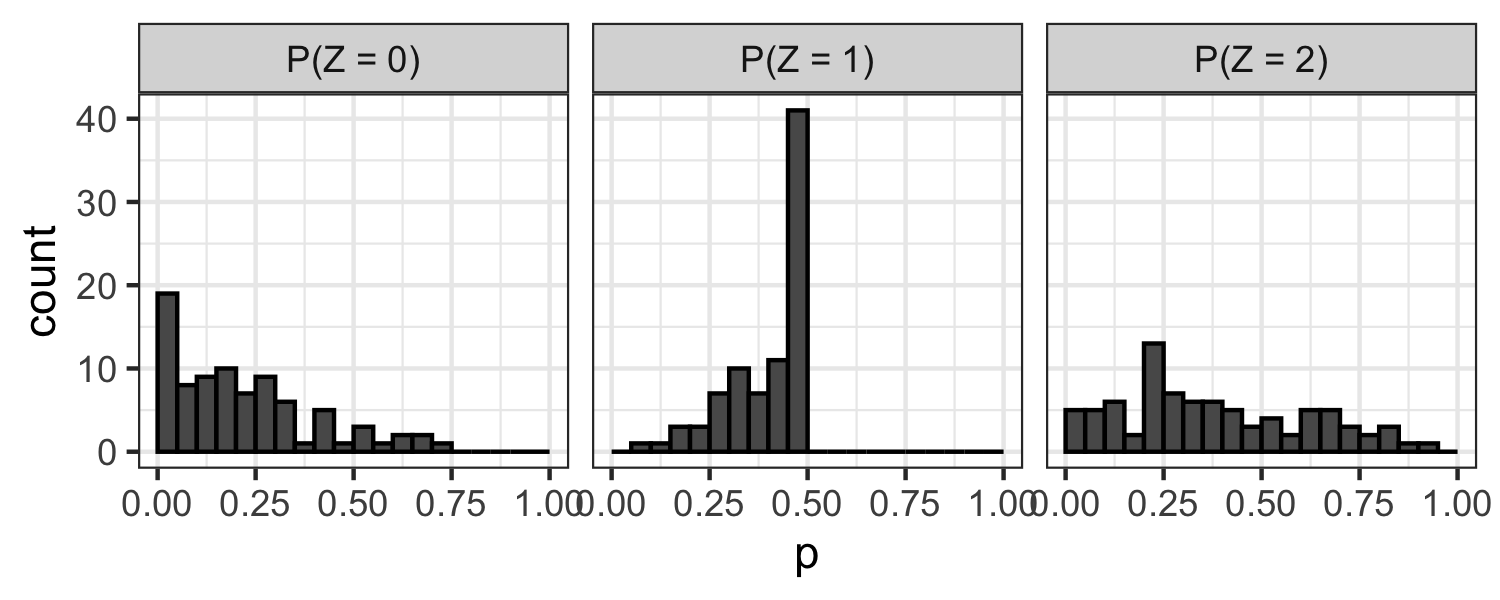
\includegraphics[width = \textwidth]{/Users/ralphtrane/Documents/RPackages_dev/ACEBounds/figures/example_analyses/smoking_depression_marginal_Z.png}
  \caption{Histograms of the marginal distribution of instruments, $P(Z = z), z=0,1,2$, estimated after preprocessing for analysis in Section \ref{smoking-effect-on-depression}}
  \label{fig:marginal-distribution-of-instruments-depression}
\end{figure}

\begin{table}[H]
  \caption{Table of the marginal distribution of instruments, $P(Z = z), z=0,1,2$, estimated after preprocessing for analysis in Section    \ref{smoking-effect-on-depression}}
  \label{tab:marginal-distribution-of-instruments-depression}
  \begin{minipage}{0.5\linewidth}
    \center
    \begin{table}[H]
\centering
\begin{tabular}{lrrr}
\toprule
SNP & P(Z = 2) & P(Z = 1) & P(Z = 0)\\
\midrule
rs10173733 & 0.3567595 & 0.4810680 & 0.1621726\\
rs10193706 & 0.2250921 & 0.4986932 & 0.2762147\\
rs10233018 & 0.2456177 & 0.4999613 & 0.2544211\\
rs10274594 & 0.2534258 & 0.4999767 & 0.2465975\\
rs1029986 & 0.1723555 & 0.4856034 & 0.3420411\\
\addlinespace
rs10774625 & 0.2452793 & 0.4999550 & 0.2547657\\
rs10813628 & 0.2353130 & 0.4995554 & 0.2651316\\
rs10897561 & 0.4145906 & 0.4585930 & 0.1268164\\
rs10905461 & 0.0653045 & 0.3804860 & 0.5542095\\
rs10914684 & 0.4568603 & 0.4381082 & 0.1050314\\
\addlinespace
rs10956808 & 0.3341139 & 0.4878239 & 0.1780622\\
rs11103667 & 0.6529965 & 0.3101710 & 0.0368325\\
rs11127913 & 0.3714083 & 0.4760490 & 0.1525428\\
rs11429972 & 0.1121109 & 0.4454375 & 0.4424516\\
rs11611651 & 0.8320219 & 0.1602609 & 0.0077172\\
\addlinespace
rs11631530 & 0.7776549 & 0.2083850 & 0.0139600\\
rs11646575 & 0.3152078 & 0.4924518 & 0.1923404\\
rs11693702 & 0.2857164 & 0.4976161 & 0.2166675\\
rs117435980 & 0.6997059 & 0.2735567 & 0.0267374\\
rs12042107 & 0.2018720 & 0.4948594 & 0.3032687\\
\addlinespace
rs12244388 & 0.4406271 & 0.4463408 & 0.1130321\\
rs12450028 & 0.4295142 & 0.4517182 & 0.1187675\\
rs12479064 & 0.6269478 & 0.3297051 & 0.0433471\\
rs12487411 & 0.2787537 & 0.4984352 & 0.2228111\\
rs12608052 & 0.2309196 & 0.4992427 & 0.2698378\\
\addlinespace
rs12725407 & 0.6539829 & 0.3094184 & 0.0365987\\
rs12886628 & 0.1122813 & 0.4456055 & 0.4421132\\
rs12910916 & 0.6211224 & 0.3339816 & 0.0448960\\
rs13100688 & 0.3932586 & 0.4676895 & 0.1390519\\
rs1492546 & 0.2020165 & 0.4948919 & 0.3030915\\
\addlinespace
rs1499982 & 0.0222374 & 0.2537694 & 0.7239932\\
rs1549213 & 0.1277548 & 0.4593465 & 0.4128986\\
rs1561195 & 0.2282248 & 0.4990080 & 0.2727672\\
rs1565735 & 0.6370613 & 0.3221998 & 0.0407389\\
rs16951001 & 0.3381946 & 0.4867008 & 0.1751046\\
\addlinespace
rs17003752 & 0.7422782 & 0.2385549 & 0.0191668\\
rs17151637 & 0.5169616 & 0.4040776 & 0.0789607\\
rs1899896 & 0.4936293 & 0.4179166 & 0.0884542\\
rs2240294 & 0.3090443 & 0.4937465 & 0.1972092\\
rs2416770 & 0.2198025 & 0.4980570 & 0.2821405\\
\addlinespace
rs264974 & 0.2632013 & 0.4996604 & 0.2371383\\
rs2675609 & 0.1388997 & 0.4675856 & 0.3935147\\
\bottomrule
\end{tabular}
\end{table}


  \end{minipage}
  \qquad
  \begin{minipage}{0.5\linewidth}
    \center
    \begin{table}[H]
\centering
\begin{tabular}{lrrr}
\toprule
SNP & P(Z = 2) & P(Z = 1) & P(Z = 0)\\
\midrule
rs2797116 & 0.5378179 & 0.3910856 & 0.0710965\\
rs2867749 & 0.4635738 & 0.4345775 & 0.1018487\\
rs299688 & 0.0809490 & 0.4071328 & 0.5119182\\
rs326341 & 0.2744742 & 0.4988573 & 0.2266685\\
rs35891966 & 0.8606480 & 0.1341263 & 0.0052257\\
\addlinespace
rs379525 & 0.2693148 & 0.4992814 & 0.2314038\\
rs42417 & 0.0958938 & 0.4275468 & 0.4765594\\
rs4566215 & 0.2180425 & 0.4978154 & 0.2841421\\
rs4910656 & 0.4335363 & 0.4497969 & 0.1166669\\
rs4957528 & 0.0432628 & 0.3294687 & 0.6272685\\
\addlinespace
rs523528 & 0.1717489 & 0.4853542 & 0.3428969\\
rs528301 & 0.2008634 & 0.4946289 & 0.3045076\\
rs55921136 & 0.6345353 & 0.3240838 & 0.0413808\\
rs568599 & 0.2093354 & 0.4963929 & 0.2942717\\
rs5850689 & 0.1341769 & 0.4642495 & 0.4015736\\
\addlinespace
rs60745548 & 0.0747215 & 0.3972616 & 0.5280169\\
rs6141314 & 0.5745378 & 0.3668899 & 0.0585724\\
rs6265 & 0.6582044 & 0.3061871 & 0.0356085\\
rs6433897 & 0.0693904 & 0.3880603 & 0.5425494\\
rs6676022 & 0.7719180 & 0.2133413 & 0.0147407\\
\addlinespace
rs6690680 & 0.7092842 & 0.2658119 & 0.0249040\\
rs6828849 & 0.3390095 & 0.4864715 & 0.1745191\\
rs71550128 & 0.2006117 & 0.4945706 & 0.3048177\\
rs72505558 & 0.3617365 & 0.4794177 & 0.1588458\\
rs72678864 & 0.6820022 & 0.2876641 & 0.0303337\\
\addlinespace
rs7333559 & 0.0438714 & 0.3311672 & 0.6249614\\
rs7451586 & 0.3546216 & 0.4817591 & 0.1636193\\
rs748828 & 0.5136337 & 0.4060975 & 0.0802688\\
rs7528604 & 0.3204723 & 0.4912608 & 0.1882668\\
rs7567570 & 0.0300586 & 0.2866312 & 0.6833102\\
\addlinespace
rs763053 & 0.6007027 & 0.3486949 & 0.0506025\\
rs76608582 & 0.9065935 & 0.0911171 & 0.0022894\\
rs772921 & 0.4307261 & 0.4511423 & 0.1181316\\
rs77878475 & 0.8356274 & 0.1569984 & 0.0073742\\
rs7870475 & 0.2766026 & 0.4986552 & 0.2247422\\
\addlinespace
rs7948789 & 0.3779911 & 0.4736374 & 0.1483715\\
rs883403 & 0.7155911 & 0.2606702 & 0.0237388\\
rs9375371 & 0.5339661 & 0.3935275 & 0.0725064\\
rs9381917 & 0.8061282 & 0.1834365 & 0.0104354\\
rs9423279 & 0.1176593 & 0.4507114 & 0.4316293\\
\addlinespace
rs9487626 & 0.0333177 & 0.2984272 & 0.6682551\\
rs9835772 & 0.5732121 & 0.3677912 & 0.0589967\\
\bottomrule
\end{tabular}
\end{table}


  \end{minipage}
\end{table}

\begin{figure}[H]
  \center
  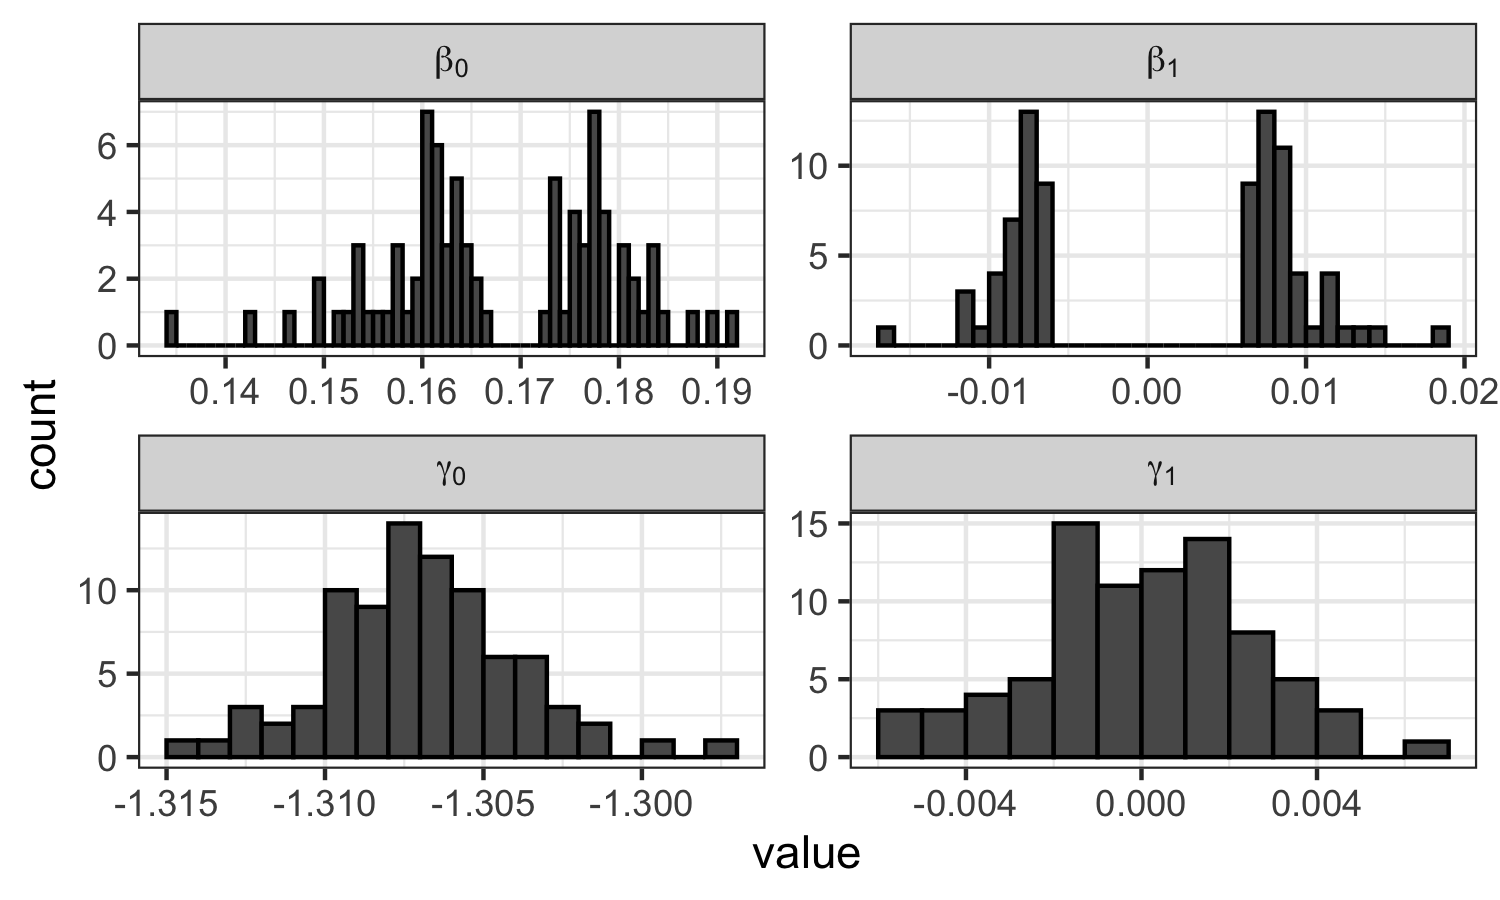
\includegraphics[width = \textwidth]{/Users/ralphtrane/Documents/RPackages_dev/ACEBounds/figures/example_analyses/smoking_depression_coefficients.png}
  \caption{Histograms of the coefficients from GWAS results of logistic regression of the SNPs on smoking status and depression status, respectively. Intercepts ($\beta_0$ and $\gamma_0$) are inferred, while slopes ($\beta_1$ and $\gamma_1$) are as reported.}
  \label{fig:marginal-distribution-of-coefficients-depression}
\end{figure}

\begin{longtable}[t]{lrrrr}
\caption{\label{tab:coefficients-depression}Coefficients from GWAS results of logistic regression of the SNPs on smoking status and depression status. Intercepts ($\beta_0$ and $\gamma_0$) are inferred, while slopes ($\beta_1$ and $\gamma_1$) are as reported.}\\
\toprule
SNP & $\beta_1$ & $\beta_0$ & $\gamma_1$ & $\gamma_0$\\
\midrule
\endfirsthead
\caption[]{\label{tab:coefficients-depression}Coefficients from GWAS results of logistic regression of the SNPs on smoking status and depression status. Intercepts ($\beta_0$ and $\gamma_0$) are inferred, while slopes ($\beta_1$ and $\gamma_1$) are as reported. \textit{(continued)}}\\
\toprule
SNP & $\beta_1$ & $\beta_0$ & $\gamma_1$ & $\gamma_0$\\
\midrule
\endhead

\endfoot
\bottomrule
\endlastfoot
rs10173733 & -0.0065148 & 0.1773825 & -0.0005704 & -1.306311\\
rs10193706 & -0.0117667 & 0.1807672 & 0.0013967 & -1.308318\\
rs10233018 & -0.0076551 & 0.1771881 & 0.0067789 & -1.313719\\
rs10274594 & 0.0078326 & 0.1617143 & 0.0012819 & -1.308284\\
rs1029986 & -0.0070208 & 0.1754296 & 0.0045713 & -1.310792\\
\addlinespace
rs10774625 & 0.0074868 & 0.1621846 & -0.0006839 & -1.306315\\
rs10813628 & -0.0068761 & 0.1762712 & 0.0027284 & -1.309641\\
rs10897561 & -0.0066917 & 0.1782175 & 0.0016886 & -1.309168\\
rs10905461 & 0.0072731 & 0.1658828 & -0.0032370 & -1.305339\\
rs10914684 & 0.0077356 & 0.1591430 & -0.0011037 & -1.305501\\
\addlinespace
rs10956808 & 0.0076247 & 0.1607859 & 0.0000764 & -1.307081\\
rs11103667 & -0.0086047 & 0.1835067 & 0.0046866 & -1.314570\\
rs11127913 & 0.0081801 & 0.1596300 & 0.0021709 & -1.309640\\
rs11429972 & 0.0083148 & 0.1640324 & -0.0016042 & -1.305919\\
rs11611651 & -0.0119868 & 0.1914677 & 0.0004842 & -1.307876\\
\addlinespace
rs11631530 & -0.0099863 & 0.1872129 & -0.0044324 & -1.299176\\
rs11646575 & -0.0082446 & 0.1788582 & 0.0009492 & -1.308059\\
rs11693702 & -0.0080254 & 0.1781801 & 0.0020852 & -1.309223\\
rs117435980 & -0.0092037 & 0.1849976 & -0.0005583 & -1.306059\\
rs12042107 & 0.0071759 & 0.1631519 & 0.0017794 & -1.308592\\
\addlinespace
rs12244388 & -0.0104344 & 0.1834539 & -0.0006776 & -1.306093\\
rs12450028 & -0.0070626 & 0.1788573 & -0.0010781 & -1.305580\\
rs12479064 & -0.0080362 & 0.1823262 & 0.0003346 & -1.307523\\
rs12487411 & 0.0075048 & 0.1616757 & -0.0035878 & -1.303206\\
rs12608052 & 0.0067542 & 0.1631088 & -0.0003997 & -1.306609\\
\addlinespace
rs12725407 & 0.0081386 & 0.1564368 & -0.0012532 & -1.304966\\
rs12886628 & -0.0071010 & 0.1743590 & 0.0007171 & -1.307473\\
rs12910916 & -0.0090138 & 0.1838081 & 0.0029727 & -1.311680\\
rs13100688 & 0.0072663 & 0.1604867 & -0.0026558 & -1.303662\\
rs1492546 & -0.0068801 & 0.1757849 & -0.0005566 & -1.306493\\
\addlinespace
rs1499982 & -0.0114648 & 0.1730198 & 0.0012934 & -1.307379\\
rs1549213 & 0.0085270 & 0.1635050 & -0.0050107 & -1.303414\\
rs1561195 & -0.0078947 & 0.1771435 & 0.0015938 & -1.308516\\
rs1565735 & 0.0115901 & 0.1510995 & 0.0017941 & -1.309857\\
rs16951001 & -0.0066035 & 0.1772805 & 0.0019827 & -1.309300\\
\addlinespace
rs17003752 & 0.0098606 & 0.1526093 & 0.0003979 & -1.307678\\
rs17151637 & 0.0075112 & 0.1587990 & 0.0038108 & -1.312475\\
rs1899896 & -0.0079928 & 0.1808315 & 0.0040686 & -1.312712\\
rs2240294 & 0.0069566 & 0.1618656 & -0.0015763 & -1.305240\\
rs2416770 & -0.0064888 & 0.1756844 & 0.0016061 & -1.308499\\
\addlinespace
rs264974 & 0.0093111 & 0.1600472 & -0.0048647 & -1.302004\\
rs2675609 & 0.0081586 & 0.1635192 & -0.0005645 & -1.306572\\
rs2797116 & 0.0079136 & 0.1579931 & -0.0039810 & -1.301155\\
rs2867749 & 0.0069446 & 0.1601434 & 0.0030286 & -1.311119\\
rs299688 & -0.0072721 & 0.1737381 & 0.0008008 & -1.307449\\
\addlinespace
rs326341 & 0.0065809 & 0.1627046 & -0.0024786 & -1.304396\\
rs35891966 & 0.0147752 & 0.1421862 & -0.0050131 & -1.297691\\
rs379525 & -0.0064906 & 0.1763367 & 0.0020069 & -1.309077\\
rs42417 & -0.0070331 & 0.1739558 & 0.0013904 & -1.307854\\
rs4566215 & 0.0066219 & 0.1634159 & -0.0011016 & -1.305964\\
\addlinespace
rs4910656 & 0.0068438 & 0.1605877 & -0.0003634 & -1.306514\\
rs4957528 & -0.0084750 & 0.1731257 & 0.0023700 & -1.307979\\
rs523528 & 0.0080708 & 0.1629110 & -0.0015950 & -1.305671\\
rs528301 & -0.0086008 & 0.1773101 & -0.0017745 & -1.305403\\
rs55921136 & 0.0085950 & 0.1559070 & -0.0002822 & -1.306543\\
\addlinespace
rs568599 & -0.0067027 & 0.1757335 & 0.0008926 & -1.307810\\
rs5850689 & 0.0119733 & 0.1608303 & -0.0020322 & -1.305504\\
rs60745548 & 0.0071946 & 0.1656667 & -0.0050431 & -1.304238\\
rs6141314 & -0.0080616 & 0.1818212 & 0.0017309 & -1.309617\\
rs6265 & 0.0101598 & 0.1531153 & 0.0034332 & -1.312565\\
\addlinespace
rs6433897 & -0.0072353 & 0.1734119 & 0.0030499 & -1.308601\\
rs6676022 & 0.0115926 & 0.1492301 & 0.0011867 & -1.309078\\
rs6690680 & 0.0088409 & 0.1547086 & -0.0012510 & -1.304886\\
rs6828849 & 0.0067122 & 0.1617838 & -0.0017619 & -1.304941\\
rs71550128 & -0.0073950 & 0.1762247 & 0.0013614 & -1.308213\\
\addlinespace
rs72505558 & 0.0067437 & 0.1614881 & 0.0004530 & -1.307538\\
rs72678864 & 0.0097538 & 0.1534904 & -0.0012454 & -1.304936\\
rs7333559 & 0.0080523 & 0.1662269 & 0.0023047 & -1.307959\\
rs7451586 & -0.0066732 & 0.1775479 & -0.0000777 & -1.306900\\
rs748828 & 0.0086213 & 0.1572430 & -0.0006899 & -1.306004\\
\addlinespace
rs7528604 & 0.0068658 & 0.1618266 & -0.0045708 & -1.301820\\
rs7567570 & -0.0091324 & 0.1727668 & 0.0007640 & -1.307258\\
rs763053 & 0.0080618 & 0.1571035 & -0.0026821 & -1.302836\\
rs76608582 & 0.0182891 & 0.1347725 & 0.0020679 & -1.310931\\
rs772921 & 0.0072725 & 0.1600543 & 0.0018384 & -1.309406\\
\addlinespace
rs77878475 & 0.0125950 & 0.1465734 & -0.0021281 & -1.303102\\
rs7870475 & -0.0071900 & 0.1771631 & 0.0004378 & -1.307453\\
rs7948789 & -0.0161713 & 0.1894889 & 0.0032357 & -1.310973\\
rs883403 & 0.0094240 & 0.1536561 & -0.0018273 & -1.303901\\
rs9375371 & -0.0073963 & 0.1804094 & -0.0032165 & -1.302293\\
\addlinespace
rs9381917 & 0.0112569 & 0.1493862 & -0.0019346 & -1.303519\\
rs9423279 & 0.0076695 & 0.1643388 & -0.0015234 & -1.305948\\
rs9487626 & 0.0131029 & 0.1648180 & -0.0015171 & -1.306439\\
rs9835772 & -0.0078024 & 0.1814146 & 0.0006795 & -1.308022\\*
\end{longtable}

\begin{figure}[H]
  \center
  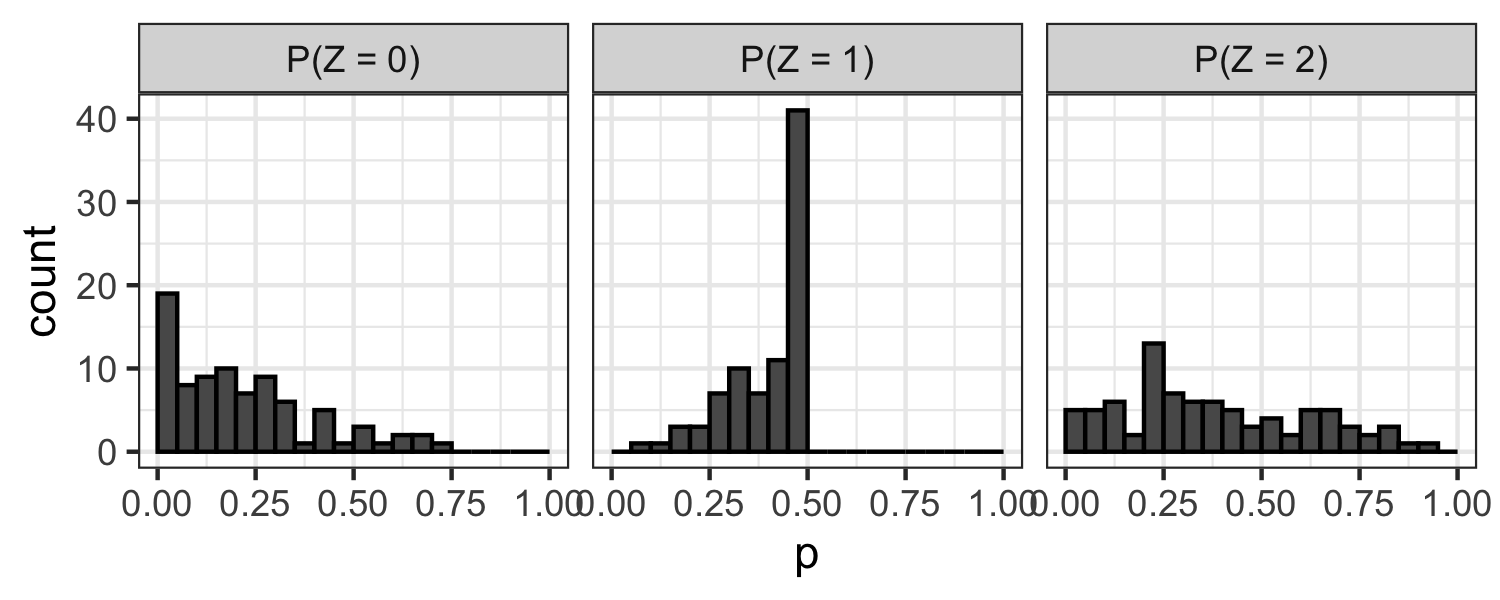
\includegraphics[width = \textwidth]{/Users/ralphtrane/Documents/RPackages_dev/ACEBounds/figures/example_analyses/smoking_lung_cancer_3_marginal_Z.png}
  \caption{Histograms of the marginal distribution of instruments, $P(Z = z), z=0,1,2$, estimated after preprocessing for analysis in Section \ref{smoking-effect-on-lung-cancer}.}
  \label{fig:marginal-distribution-of-instruments-lung-cancer}
\end{figure}

\begin{table}[H]
  \caption{Table of the marginal distribution of instruments, $P(Z = z), z=0,1,2$, estimated after preprocessing for analysis in Section \ref{smoking-effect-on-lung-cancer}}
  \label{tab:marginal-distribution-of-instruments-lung-cancer}
  \begin{minipage}{0.5\linewidth}
    \center
    \begin{table}[H]
\centering
\begin{tabular}{lrrr}
\toprule
SNP & P(Z = 2) & P(Z = 1) & P(Z = 0)\\
\midrule
rs10173733 & 0.3562119 & 0.4812460 & 0.1625421\\
rs10193706 & 0.2254196 & 0.4987283 & 0.2758521\\
rs10233018 & 0.2458307 & 0.4999649 & 0.2542044\\
rs10274594 & 0.2540510 & 0.4999674 & 0.2459816\\
rs1029986 & 0.1723980 & 0.4856208 & 0.3419813\\
\addlinespace
rs10774625 & 0.2457332 & 0.4999633 & 0.2543035\\
rs10813628 & 0.2349574 & 0.4995333 & 0.2655093\\
rs10897561 & 0.4140371 & 0.4588401 & 0.1271228\\
rs10905461 & 0.0654474 & 0.3807590 & 0.5537936\\
rs10914684 & 0.4570550 & 0.4380069 & 0.1049382\\
\addlinespace
rs10956808 & 0.3337643 & 0.4879181 & 0.1783175\\
rs11103667 & 0.6528207 & 0.3103050 & 0.0368743\\
rs11127913 & 0.3717426 & 0.4759287 & 0.1523286\\
rs11429972 & 0.1128192 & 0.4461330 & 0.4410478\\
rs11611651 & 0.8323808 & 0.1599365 & 0.0076827\\
\addlinespace
rs11631530 & 0.7779345 & 0.2081429 & 0.0139226\\
rs11646575 & 0.3149600 & 0.4925059 & 0.1925340\\
rs11693702 & 0.2849095 & 0.4977193 & 0.2173712\\
rs117435980 & 0.6998026 & 0.2734789 & 0.0267185\\
rs12042107 & 0.2025948 & 0.4950210 & 0.3023842\\
\addlinespace
rs12244388 & 0.4404143 & 0.4464457 & 0.1131399\\
rs12450028 & 0.4293549 & 0.4517938 & 0.1188513\\
rs12479064 & 0.6268375 & 0.3297864 & 0.0433761\\
rs12487411 & 0.2788384 & 0.4984262 & 0.2227354\\
rs12608052 & 0.2306302 & 0.4992191 & 0.2701507\\
\addlinespace
rs12725407 & 0.6546886 & 0.3088794 & 0.0364320\\
rs12886628 & 0.1124522 & 0.4457734 & 0.4417744\\
rs12910916 & 0.6206505 & 0.3343265 & 0.0450230\\
rs13100688 & 0.3932914 & 0.4676762 & 0.1390324\\
rs1492546 & 0.2022894 & 0.4949531 & 0.3027575\\
\addlinespace
rs1499982 & 0.0221071 & 0.2531548 & 0.7247382\\
rs1549213 & 0.1285982 & 0.4600154 & 0.4113864\\
rs1561195 & 0.2279701 & 0.4989841 & 0.2730458\\
rs1565735 & 0.6376078 & 0.3217914 & 0.0406009\\
rs16951001 & 0.3380123 & 0.4867519 & 0.1752358\\
\addlinespace
rs17003752 & 0.7420669 & 0.2387323 & 0.0192008\\
rs17151637 & 0.5166809 & 0.4042486 & 0.0790705\\
rs1899896 & 0.4934387 & 0.4180265 & 0.0885349\\
rs2240294 & 0.3093641 & 0.4936820 & 0.1969539\\
rs2416770 & 0.2199058 & 0.4980707 & 0.2820235\\
\addlinespace
rs264974 & 0.2640248 & 0.4996173 & 0.2363579\\
rs2675609 & 0.1387352 & 0.4674731 & 0.3937917\\
\bottomrule
\end{tabular}
\end{table}


  \end{minipage}
  \qquad
  \begin{minipage}{0.5\linewidth}
    \center
    \begin{table}[H]
\centering
\begin{tabular}{lrrr}
\toprule
SNP & P(Z = 2) & P(Z = 1) & P(Z = 0)\\
\midrule
rs2797116 & 0.5370791 & 0.3915554 & 0.0713655\\
rs2867749 & 0.4639468 & 0.4343792 & 0.1016740\\
rs299688 & 0.0806544 & 0.4066855 & 0.5126601\\
rs326341 & 0.2745833 & 0.4988473 & 0.2265693\\
rs35891966 & 0.8609698 & 0.1338295 & 0.0052006\\
\addlinespace
rs379525 & 0.2690001 & 0.4993042 & 0.2316957\\
rs42417 & 0.0959979 & 0.4276747 & 0.4763274\\
rs4566215 & 0.2184561 & 0.4978736 & 0.2836703\\
rs4910656 & 0.4334112 & 0.4498570 & 0.1167317\\
rs4957528 & 0.0432505 & 0.3294341 & 0.6273153\\
\addlinespace
rs523528 & 0.1717181 & 0.4853414 & 0.3429405\\
rs528301 & 0.2006916 & 0.4945891 & 0.3047192\\
rs55921136 & 0.6351822 & 0.3236020 & 0.0412158\\
rs568599 & 0.2090011 & 0.4963306 & 0.2946684\\
rs5850689 & 0.1341980 & 0.4642649 & 0.4015371\\
\addlinespace
rs60745548 & 0.0747101 & 0.3972427 & 0.5280472\\
rs6141314 & 0.5735637 & 0.3675524 & 0.0588839\\
rs6265 & 0.6582586 & 0.3061456 & 0.0355959\\
rs6433897 & 0.0693372 & 0.3879647 & 0.5426982\\
rs6676022 & 0.7713790 & 0.2138057 & 0.0148153\\
\addlinespace
rs6690680 & 0.7094689 & 0.2656618 & 0.0248694\\
rs6828849 & 0.3395694 & 0.4863129 & 0.1741177\\
rs71550128 & 0.2008017 & 0.4946147 & 0.3045837\\
rs72505558 & 0.3617072 & 0.4794276 & 0.1588652\\
rs72678864 & 0.6825787 & 0.2872090 & 0.0302123\\
\addlinespace
rs7333559 & 0.0439935 & 0.3315056 & 0.6245008\\
rs7451586 & 0.3541182 & 0.4819202 & 0.1639616\\
rs748828 & 0.5139770 & 0.4058898 & 0.0801332\\
rs7528604 & 0.3213716 & 0.4910497 & 0.1875787\\
rs7567570 & 0.0299625 & 0.2862686 & 0.6837689\\
\addlinespace
rs763053 & 0.6013164 & 0.3482591 & 0.0504245\\
rs76608582 & 0.9070039 & 0.0907272 & 0.0022689\\
rs772921 & 0.4315416 & 0.4507533 & 0.1177051\\
rs77878475 & 0.8356836 & 0.1569474 & 0.0073690\\
rs7870475 & 0.2763346 & 0.4986816 & 0.2249839\\
\addlinespace
rs7948789 & 0.3767706 & 0.4740916 & 0.1491378\\
rs883403 & 0.7156415 & 0.2606289 & 0.0237296\\
rs9375371 & 0.5345687 & 0.3931467 & 0.0722846\\
rs9381917 & 0.8063218 & 0.1832649 & 0.0104133\\
rs9423279 & 0.1179428 & 0.4509704 & 0.4310869\\
\addlinespace
rs9487626 & 0.0332246 & 0.2981030 & 0.6686724\\
rs9835772 & 0.5737177 & 0.3674477 & 0.0588346\\
\bottomrule
\end{tabular}
\end{table}


  \end{minipage}
\end{table}

\begin{figure}[H]
  \center
  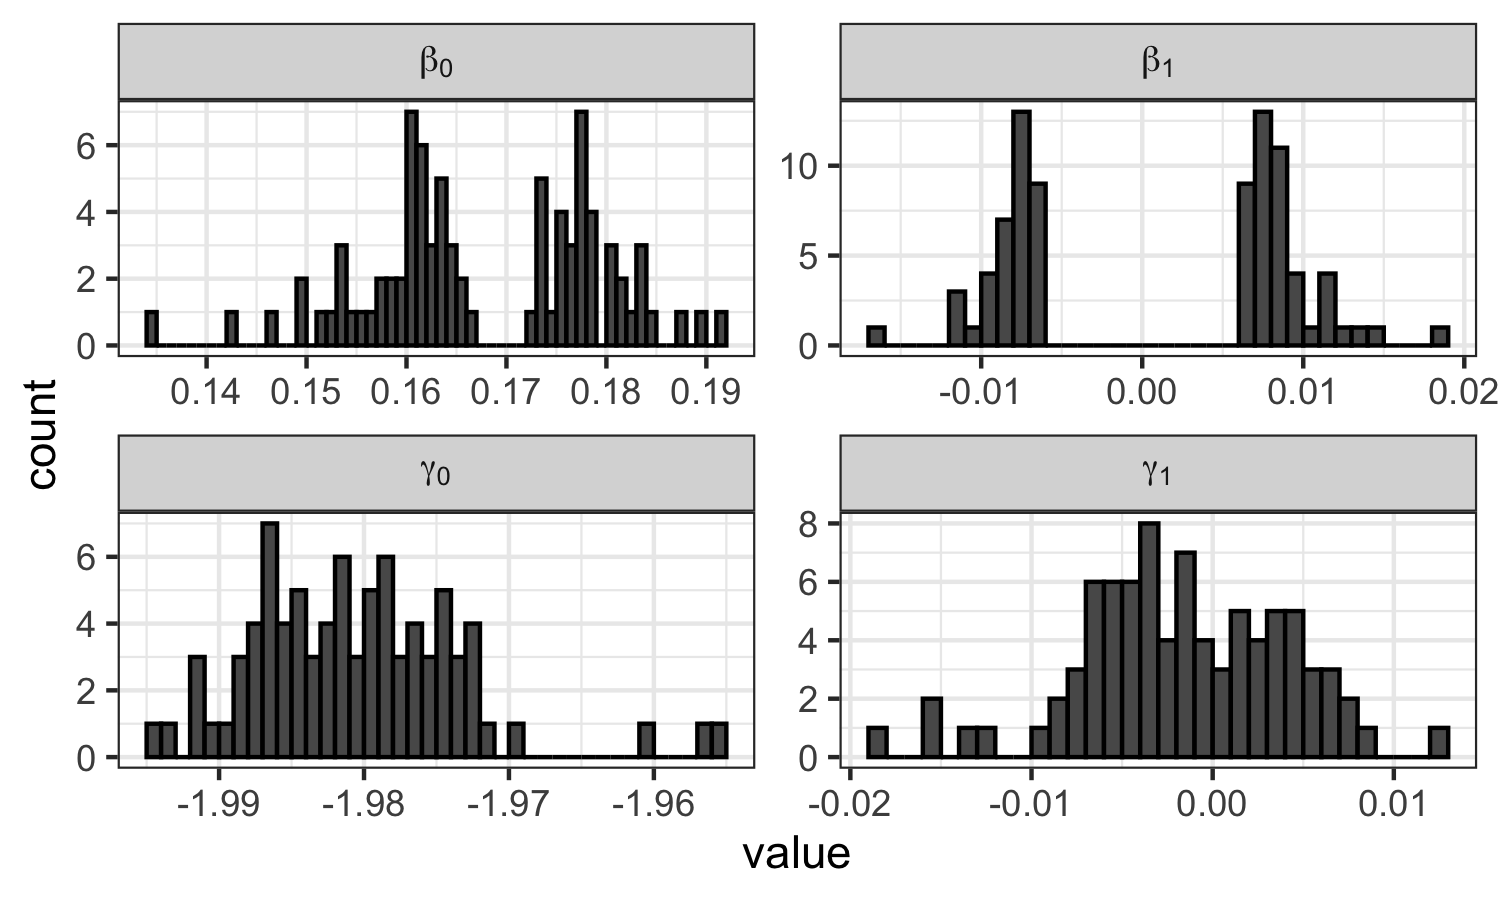
\includegraphics[width = \textwidth]{/Users/ralphtrane/Documents/RPackages_dev/ACEBounds/figures/example_analyses/smoking_lung_cancer_3_coefficients.png}
  \caption{Histograms of the coefficients from GWAS results of logistic regression of the SNPs on smoking status and lung cancer status. Intercepts ($\beta_0$ and $\gamma_0$) are inferred, while slopes ($\beta_1$ and $\gamma_1$) are as reported.}
  \label{fig:marginal-distribution-of-coefficients-lung-cancer}
\end{figure}

\begin{longtable}[t]{lrrrr}
\caption{\label{tab:coefficients-lung-cancer}Coefficients from GWAS results of logistic regression of the SNPs on smoking status and lung cancer status. Intercepts ($\beta_0$ and $\gamma_0$) are inferred, while slopes ($\beta_1$ and $\gamma_1$) are as reported.}\\
\toprule
SNP & $\beta_1$ & $\beta_0$ & $\gamma_1$ & $\gamma_0$\\
\midrule
\endfirsthead
\caption[]{\label{tab:coefficients-lung-cancer}Coefficients from GWAS results of logistic regression of the SNPs on smoking status and lung cancer status. Intercepts ($\beta_0$ and $\gamma_0$) are inferred, while slopes ($\beta_1$ and $\gamma_1$) are as reported. \textit{(continued)}}\\
\toprule
SNP & $\beta_1$ & $\beta_0$ & $\gamma_1$ & $\gamma_0$\\
\midrule
\endhead

\endfoot
\bottomrule
\endlastfoot
rs10173733 & -0.0065148 & 0.1773766 & 0.0033363 & -1.987122\\
rs10193706 & -0.0117667 & 0.1807753 & -0.0015310 & -1.981684\\
rs10233018 & -0.0076551 & 0.1771914 & 0.0050495 & -1.988150\\
rs10274594 & 0.0078326 & 0.1617046 & -0.0015364 & -1.981589\\
rs1029986 & -0.0070208 & 0.1754303 & 0.0035498 & -1.986088\\
\addlinespace
rs10774625 & 0.0074868 & 0.1621777 & -0.0084158 & -1.974806\\
rs10813628 & -0.0068761 & 0.1762662 & 0.0051706 & -1.988156\\
rs10897561 & -0.0066917 & 0.1782117 & 0.0066835 & -1.991747\\
rs10905461 & 0.0072731 & 0.1658787 & -0.0058844 & -1.980131\\
rs10914684 & 0.0077356 & 0.1591408 & -0.0026047 & -1.979616\\
\addlinespace
rs10956808 & 0.0076247 & 0.1607905 & -0.0063546 & -1.975802\\
rs11103667 & -0.0086047 & 0.1835048 & 0.0063118 & -1.993343\\
rs11127913 & 0.0081801 & 0.1596256 & -0.0033969 & -1.978997\\
rs11429972 & 0.0083148 & 0.1640148 & -0.0096129 & -1.976695\\
rs11611651 & -0.0119868 & 0.1914724 & 0.0013059 & -1.985521\\
\addlinespace
rs11631530 & -0.0099863 & 0.1872160 & -0.0047887 & -1.974691\\
rs11646575 & -0.0082446 & 0.1788545 & 0.0012319 & -1.984521\\
rs11693702 & -0.0080254 & 0.1781679 & 0.0046224 & -1.988077\\
rs117435980 & -0.0092037 & 0.1849986 & -0.0054804 & -1.973970\\
rs12042107 & 0.0071759 & 0.1631404 & -0.0020557 & -1.981288\\
\addlinespace
rs12244388 & -0.0104344 & 0.1834505 & 0.0019355 & -1.985707\\
rs12450028 & -0.0070626 & 0.1788556 & -0.0024536 & -1.979923\\
rs12479064 & -0.0080362 & 0.1823251 & -0.0088600 & -1.969116\\
rs12487411 & 0.0075048 & 0.1616745 & -0.0077980 & -1.974913\\
rs12608052 & 0.0067542 & 0.1631129 & -0.0048100 & -1.978521\\
\addlinespace
rs12725407 & 0.0081386 & 0.1564297 & -0.0067998 & -1.972138\\
rs12886628 & -0.0071010 & 0.1743626 & -0.0018595 & -1.981891\\
rs12910916 & -0.0090138 & 0.1838027 & 0.0026458 & -1.987308\\
rs13100688 & 0.0072663 & 0.1604864 & -0.0055464 & -1.976186\\
rs1492546 & -0.0068801 & 0.1757890 & 0.0040638 & -1.986797\\
\addlinespace
rs1499982 & -0.0114648 & 0.1730098 & 0.0024892 & -1.983878\\
rs1549213 & 0.0085270 & 0.1634849 & 0.0056335 & -1.987184\\
rs1561195 & -0.0078947 & 0.1771393 & 0.0072232 & -1.990046\\
rs1565735 & 0.0115901 & 0.1510915 & -0.0072487 & -1.971566\\
rs16951001 & -0.0066035 & 0.1772784 & 0.0070226 & -1.991313\\
\addlinespace
rs17003752 & 0.0098606 & 0.1526117 & -0.0055424 & -1.973591\\
rs17151637 & 0.0075112 & 0.1588020 & -0.0027771 & -1.979146\\
rs1899896 & -0.0079928 & 0.1808293 & 0.0047935 & -1.989876\\
rs2240294 & 0.0069566 & 0.1618616 & -0.0078381 & -1.974429\\
rs2416770 & -0.0064888 & 0.1756858 & -0.0035668 & -1.979794\\
\addlinespace
rs264974 & 0.0093111 & 0.1600323 & -0.0047198 & -1.978291\\
rs2675609 & 0.0081586 & 0.1635228 & -0.0069708 & -1.977953\\
rs2797116 & 0.0079136 & 0.1580011 & -0.0039635 & -1.977330\\
rs2867749 & 0.0069446 & 0.1601396 & -0.0032894 & -1.978658\\
rs299688 & -0.0072721 & 0.1737306 & -0.0019058 & -1.982055\\
\addlinespace
rs326341 & 0.0065809 & 0.1627032 & 0.0031753 & -1.986468\\
rs35891966 & 0.0147752 & 0.1421811 & -0.0122161 & -1.960473\\
rs379525 & -0.0064906 & 0.1763327 & -0.0018594 & -1.981209\\
rs42417 & -0.0070331 & 0.1739582 & 0.0003829 & -1.983375\\
rs4566215 & 0.0066219 & 0.1634100 & -0.0035546 & -1.979817\\
\addlinespace
rs4910656 & 0.0068438 & 0.1605890 & -0.0006962 & -1.982221\\
rs4957528 & -0.0084750 & 0.1731252 & 0.0036288 & -1.984649\\
rs523528 & 0.0080708 & 0.1629116 & 0.0029251 & -1.985564\\
rs528301 & -0.0086008 & 0.1773068 & 0.0124616 & -1.994333\\
rs55921136 & 0.0085950 & 0.1559000 & -0.0069653 & -1.972040\\
\addlinespace
rs568599 & -0.0067027 & 0.1757286 & 0.0043346 & -1.987105\\
rs5850689 & 0.0119733 & 0.1608296 & -0.0038879 & -1.980291\\
rs60745548 & 0.0071946 & 0.1656670 & 0.0062353 & -1.986552\\
rs6141314 & -0.0080616 & 0.1818108 & 0.0010534 & -1.984733\\
rs6265 & 0.0101598 & 0.1531146 & -0.0043806 & -1.976031\\
\addlinespace
rs6433897 & -0.0072353 & 0.1734104 & -0.0011588 & -1.982527\\
rs6676022 & 0.0115926 & 0.1492373 & -0.0153059 & -1.956268\\
rs6690680 & 0.0088409 & 0.1547067 & -0.0050219 & -1.974679\\
rs6828849 & 0.0067122 & 0.1617773 & 0.0008050 & -1.984076\\
rs71550128 & -0.0073950 & 0.1762278 & 0.0034139 & -1.986200\\
\addlinespace
rs72505558 & 0.0067437 & 0.1614885 & -0.0009876 & -1.981950\\
rs72678864 & 0.0097538 & 0.1534836 & -0.0034394 & -1.977455\\
rs7333559 & 0.0080523 & 0.1662222 & -0.0183846 & -1.975467\\
rs7451586 & -0.0066732 & 0.1775422 & 0.0027432 & -1.986404\\
rs748828 & 0.0086213 & 0.1572389 & -0.0047229 & -1.976368\\
\addlinespace
rs7528604 & 0.0068658 & 0.1618157 & -0.0001820 & -1.982931\\
rs7567570 & -0.0091324 & 0.1727617 & -0.0002451 & -1.983053\\
rs763053 & 0.0080618 & 0.1570972 & -0.0069210 & -1.972409\\
rs76608582 & 0.0182891 & 0.1347646 & -0.0048192 & -1.973958\\
rs772921 & 0.0072725 & 0.1600453 & -0.0054837 & -1.975937\\
\addlinespace
rs77878475 & 0.0125950 & 0.1465726 & 0.0010985 & -1.985146\\
rs7870475 & -0.0071900 & 0.1771594 & 0.0082598 & -1.991835\\
rs7948789 & -0.0161713 & 0.1894568 & 0.0009336 & -1.984284\\
rs883403 & 0.0094240 & 0.1536556 & -0.0014726 & -1.980646\\
rs9375371 & -0.0073963 & 0.1804155 & -0.0069852 & -1.972929\\
\addlinespace
rs9381917 & 0.0112569 & 0.1493838 & -0.0155636 & -1.955201\\
rs9423279 & 0.0076695 & 0.1643324 & 0.0046716 & -1.986350\\
rs9487626 & 0.0131029 & 0.1648247 & -0.0136868 & -1.978168\\
rs9835772 & -0.0078024 & 0.1814198 & -0.0031275 & -1.978401\\*
\end{longtable}

\hypertarget{references}{%
\section*{References}\label{references}}
\addcontentsline{toc}{section}{References}

\hypertarget{refs}{}
\begin{CSLReferences}{1}{0}
\leavevmode\hypertarget{ref-assarf_computing_2017}{}%
Assarf, Benjamin, Ewgenij Gawrilow, Katrin Herr, Michael Joswig, Benjamin Lorenz, Andreas Paffenholz, and Thomas Rehn. 2017. {``Computing Convex Hulls and Counting Integer Points with Polymake.''} \emph{Mathematical Programming Computation} 9 (1): 1--38. \url{https://doi.org/10.1007/s12532-016-0104-z}.

\leavevmode\hypertarget{ref-balke_nonparametric_1993}{}%
Balke, Alexander, and Judea Pearl. 1993. {``Nonparametric {Bounds} on {Causal Effects} from {Partial Compliance Data}.''} {JOURNAL OF THE AMERICAN STATISTICAL ASSOCIATION}.

\leavevmode\hypertarget{ref-balke_bounds_1997}{}%
---------. 1997. {``Bounds on {Treatment Effects} from {Studies} with {Imperfect Compliance}.''} \emph{Journal of the American Statistical Association} 92 (439): 1171--76. \url{https://doi.org/10.1080/01621459.1997.10474074}.

\leavevmode\hypertarget{ref-beck_gwas_2020}{}%
Beck, Tim, Tom Shorter, and Anthony J. Brookes. 2020. {``{GWAS Central}: A Comprehensive Resource for the Discovery and Comparison of Genotype and Phenotype Data from Genome-Wide Association Studies.''} \emph{Nucleic Acids Research} 48 (D1): D933--40. \url{https://doi.org/10.1093/nar/gkz895}.

\leavevmode\hypertarget{ref-cornfield_smoking_1959}{}%
Cornfield, Jerome, William Haenszel, E. Cuyler Hammond, Abraham M. Lilienfeld, Michael B. Shimkin, and Ernst L. Wynder. 1959. {``Smoking and {Lung Cancer}: {Recent Evidence} and a {Discussion} of {Some Questions}.''} \emph{JNCI: Journal of the National Cancer Institute} 22 (1): 173--203. \url{https://doi.org/10.1093/jnci/22.1.173}.

\leavevmode\hypertarget{ref-davies_reading_2018}{}%
Davies, Neil M., Michael V. Holmes, and George Davey Smith. 2018. {``Reading {Mendelian} Randomisation Studies: A Guide, Glossary, and Checklist for Clinicians.''} \emph{BMJ} 362 (July). \url{https://doi.org/10.1136/bmj.k601}.

\leavevmode\hypertarget{ref-erlich_routes_2014}{}%
Erlich, Yaniv, and Arvind Narayanan. 2014. {``Routes for Breaching and Protecting Genetic Privacy.''} \emph{Nature Reviews Genetics} 15 (6): 409--21. \url{https://doi.org/10.1038/nrg3723}.

\leavevmode\hypertarget{ref-fuller_privacy_1999}{}%
Fuller, B. P., M. J. Ellis Kahn, P. A. Barr, L. Biesecker, E. Crowley, J. Garber, M. K. Mansoura, et al. 1999. {``Privacy in {Genetics Research}.''} \emph{Science} 285 (5432): 1359--61. \url{https://doi.org/10.1126/science.285.5432.1359}.

\leavevmode\hypertarget{ref-mrbase}{}%
Hemani, Gibran, Jie Zheng, Benjamin Elsworth, Kaitlin H Wade, Valeriia Haberland, Denis Baird, Charles Laurin, et al. 2018. {``The MR-Base Platform Supports Systematic Causal Inference Across the Human Phenome.''} Edited by Ruth Loos. \emph{eLife} 7 (May): e34408. \url{https://doi.org/10.7554/eLife.34408}.

\leavevmode\hypertarget{ref-lawlor_mendelian_2008}{}%
Lawlor, Debbie A., Roger M. Harbord, Jonathan A. C. Sterne, Nic Timpson, and George Davey Smith. 2008. {``Mendelian Randomization: Using Genes as Instruments for Making Causal Inferences in Epidemiology.''} \emph{Statistics in Medicine} 27 (8): 1133--63. \url{https://doi.org/10.1002/sim.3034}.

\leavevmode\hypertarget{ref-manski_nonparametric_1990}{}%
Manski, Charles F. 1990. {``Nonparametric {Bounds} on {Treatment Effects}.''} \emph{The American Economic Review} 80 (2): 319--23.

\leavevmode\hypertarget{ref-marigorta_replicability_2018}{}%
Marigorta, Urko M., Juan Antonio Rodrìguez, Greg Gibson, and Arcadi Navarro. 2018. {``Replicability and {Prediction}: Lessons and Challenges from {GWAS}.''} \emph{Trends in Genetics : TIG} 34 (7): 504--17. \url{https://doi.org/10.1016/j.tig.2018.03.005}.

\leavevmode\hypertarget{ref-R}{}%
R Core Team. 2020. \emph{R: A Language and Environment for Statistical Computing}. Vienna, Austria: R Foundation for Statistical Computing. \url{https://www.R-project.org/}.

\leavevmode\hypertarget{ref-ramsahai_causal_2007}{}%
Ramsahai, Roland R. 2007. {``Causal {Bounds} and {Instruments}.''} In \emph{Proceedings of the {Twenty}-{Third Conference} on {Uncertainty} in {Artificial Intelligence}}, 310--17. {UAI}'07. {Arlington, Virginia, United States}: {AUAI Press}.

\leavevmode\hypertarget{ref-ramsahai_causal_2012}{}%
---------. 2012. {``Causal {Bounds} and {Observable Constraints} for {Non}-Deterministic {Models}.''} \emph{J. Mach. Learn. Res.} 13 (March): 829--48.

\leavevmode\hypertarget{ref-richardson_ace_2014}{}%
Richardson, Thomas S., and James M. Robins. 2014. {``{ACE Bounds}; {SEMs} with {Equilibrium Conditions}.''} \emph{Statistical Science} 29 (3): 363--66. \url{https://doi.org/10.1214/14-STS485}.

\leavevmode\hypertarget{ref-robins_analysis_1989}{}%
Robins, James M. 1989. {``The {Analysis} of {Randomized} and {Nonrandomized AIDS Treatment Trials Using A New Approach} to {Causal Inference} in {Longitudinal Studies}.''} \emph{Health Service Research Methodology: A Focus On AIDS}, 113--59.

\leavevmode\hypertarget{ref-swanson_partial_2018}{}%
Swanson, Sonja A., Miguel A. Hern'an, Matthew Miller, James M. Robins, and Thomas S. Richardson. 2018. {``Partial {Identification} of the {Average Treatment Effect Using Instrumental Variables}: {Review} of {Methods} for {Binary Instruments}, {Treatments}, and {Outcomes}.''} \emph{Journal of the American Statistical Association} 113 (522): 933--47. \url{https://doi.org/10.1080/01621459.2018.1434530}.

\leavevmode\hypertarget{ref-wang_genome_2017}{}%
Wang, Shuang, Xiaoqian Jiang, Siddharth Singh, Rebecca Marmor, Luca Bonomi, Dov Fox, Michelle Dow, and Lucila Ohno-Machado. 2017. {``Genome Privacy: Challenges, Technical Approaches to Mitigate Risk, and Ethical Considerations in the {United States}.''} \emph{Annals of the New York Academy of Sciences} 1387 (1): 73--83. \url{https://doi.org/10.1111/nyas.13259}.

\leavevmode\hypertarget{ref-wootton_evidence_2019}{}%
Wootton, Robyn E., Rebecca C. Richmond, Bobby G. Stuijfzand, Rebecca B. Lawn, Hannah M. Sallis, Gemma M. J. Taylor, Gibran Hemani, et al. 2019. {``Evidence for Causal Effects of Lifetime Smoking on Risk for Depression and Schizophrenia: A {Mendelian} Randomisation Study.''} \emph{Psychological Medicine}, September, 1--9. \url{https://doi.org/10.1017/S0033291719002678}.

\end{CSLReferences}

\end{document}
